\chapter{Estabilidad Estructural}

\section{Preliminares}


\begin{defn}[Formas $r-$lineales]
	Tomando $r \geq 2$, decimos que una función del producto de espacios vectoriales $\{ E_i\}_{i \in \{ 1,2,\dots,r\}}$ al espacio vectorial $F$
	
	\begin{equation*}
		\displaystyle M:\Pi _{i \in \{ 1,\dots,r\}} E_i\to F    
	\end{equation*}
	
	es $r-$lineal si es lineal en cada componente. Es decir, dado $i \in \{ 1,\dots, r\}$:
	
	\begin{align*}
		\forall v \in \Pi _{j \in \{ 1,\dots,i-1\}} E_i \times \{ 0_{E_i}\} \times \Pi _{j \in \{ i+1,\dots r\}} E_i, , \forall u_i, w_i \in E_i : \\ 
		M(v +\alpha  u_i  +\beta  u_i) = \alpha M(v +  u_i) + \beta M(v +  w_i)
	\end{align*}
	
	Denotamos el conjunto de formas $r-$lineales entre dos espacios como $\operatorname{Mult}^r(E_1,\dots,E_r;F)$
	
	
\end{defn}

\begin{notn}
	Cuando $r = 1$ las formas son lineales y se denota según la teoría básica del álgebra lineal $\operatorname{Mult}^1(E,F) = \operatorname{Hom}(E,F)$
	
	Cuando para algún $r$, el mapeo $M$ sea $r-$lineal entre espacios de salida $\{ E_i\}_{i \in \{ 1,2,\dots,r\}}$ y $F$; diremos que la forma es multilineal. 
	
\end{notn}

\begin{defn}[Funciones de Medidas]
	Sea $A$ conjunto y $\mathcal{S}$ familia de conjuntos. 
	
	Sea 
	
	\begin{equation*}
		\mathcal{F} = \{g : A \to X \mid X \in \mathcal{S} \}
	\end{equation*}
	
	familia de funciones con dominio $A$ y rango un miembro de $\mathcal{S}$.
	
	Sea 
	
	\begin{equation*}
		\mathcal{H} = \{\tau : X \to Y \mid X,Y \in \mathcal{S} \}  
	\end{equation*}
	
	Familia de funciones con dominio y rango en $\mathcal{S}$. 
	
	Asumimos que $\mathcal{H}$ tiene la estructura:
	
	\begin{enumerate}
		\item $\mathcal{H}$ contiene la función identidad de cada miembro de $\mathcal{S}$. $(\forall X \in \mathcal{S}, Id_X \in \mathcal{S})$
		\item $\mathcal{H}$ is cerrado bajo la operación  (asociativa) de composición de funciones.$( \mathcal{H} \circ \mathcal{H} \subseteq \mathcal{H})$
		\item Dado $\tau\in \mathcal{H}$,$f\in \mathcal{F}$, la composición $\tau \circ f$ es definida y está en $\mathcal{F}$. $( \mathcal{H} \circ \mathcal{F} \subseteq \mathcal{H})$
	\end{enumerate}
	
	
	
	Decimos que la famliia $\mathcal{H}$ es la familia de medidas y sus miembros son funciones de medidas.
	
	Un par $(S, f:A\to S)$, donde  $S \in \mathcal{S}$ y $f = \mathcal{F}$, tiene la propiedad universal para la familia $\mathcal{F}$, o es un par universal para $(\mathcal{F},\mathcal{H})$, si:
	
	
	\begin{equation*}
		\forall (g : A\to X) \in \mathcal{F}, \exists ! (\tau : S\to X )\in \mathcal{H}: g = \tau  \circ f
	\end{equation*} 
	
	Si acontece, se dice que todo $g \in \mathcal{F}$ puede ser factorado mediante $f$.
	
	La única función de medidas $\tau$ se dice morfismo mediante para $g$
	
	
\end{defn}

\begin{rmrk}
	La idea central detrás de factorar es poder distinguir con las funciones en los valores de $A$ la información distinta (que vamos a medir). Por tanto lo que g distinga, f distinguirá (y esa distinción o comparación será nuestra medida, que no debe confundirse con teoría de la medida).
	
	Es decir: $f(x) = f(y) \Rightarrow \tau (f(x)) = \tau(f(y)) \Rightarrow g(x) = g(y)$
	
	Luego: $g(x) \neq g(y) \Rightarrow f(x) \neq f(y)$
	
	
	Luego el dato: "$x,y$ son distintos para la función $g$" implica el dato: "$x,y$ son distintos para la función $f$".
	
	Si $\tau$ es inyectivo, la única diferencia entre $f,g$ es el valor de las etiquetas o valores de imagen.
	
	Normalmente $\tau$ puede ser no inyectiva, en cuyo caso $f$ contiene más información que $g$.
\end{rmrk}

\begin{visua}
	Tomemos el siguiente diagrama para visualizar como $\mathcal{H}$ mide de forma más "universal" la información de los $g$ en $\mathcal{F}$
	
	
	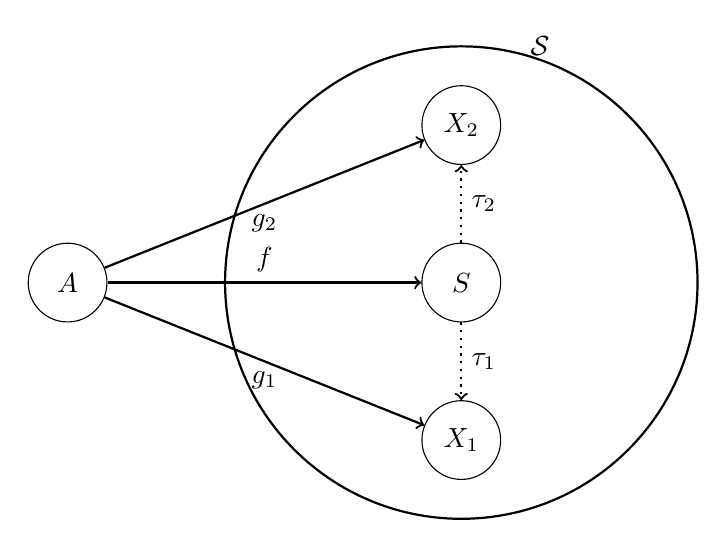
\begin{tikzpicture}[scale=1]
		
		% Nodo A
		\node[circle, draw, minimum size=1cm] (A) at (0,0) {\( A \)};
		
		% Conjunto universal U
		\draw[thick] (5,0) circle [radius=3];
		\node at (6,3)  {\( \mathcal{S}\)};
		
		% Subconjuntos S y X dentro de U
		\node[circle, draw, minimum size=1cm] (S) at (5,0) {\( S \)};
		\node[circle, draw, minimum size=1cm] (X1) at (5,-2) {\( X_1 \)};
		\node[circle, draw, minimum size=1cm] (X2) at (5,2) {\( X_2 \)};
		
		
		% Flechas desde A
		\draw[->, thick] (A) -- (S) node[midway, above] {\( f \)};
		\draw[->, thick] (A) -- (X1) node[midway, below] {\( g_1 \)};
		\draw[->, thick] (A) -- (X2) node[midway, below] {\( g_2 \)};
		
		% Flecha de S a X
		\draw[->, thick,dotted] (S) -- (X1) node[midway, right] {\( \tau_1 \)};
		\draw[->, thick,dotted] (S) -- (X2) node[midway, right] {\( \tau_2 \)};
		
	\end{tikzpicture}
	
	Con el diagrama se ve que para el par universal, $f$ es el centro de todas las funciones en $\mathcal{F}$. Conteniendo más información que las demás.
\end{visua}


\begin{thm}[Unicidad de Pares Universales]
	Sean $(S,f:A\to S), (T,g:A\to T)$ pares universales para $(\mathcal{F},\mathcal{H})$. 
	
	Existe una función de medidas biyectiva $\mu \in \mathcal{H}$ para la cual $\mu (S) = T$.
	
	El morfismo mediante de $f$ con respecto de $g$ y el morfismo mediante de $g$ con respecto de $f$ son isomorfismos y son el inverso de cada uno con respecto del otro.
	
	De acuerdo al diagrama anterior, si tenemos dos centros, podemos crear un isomorfismo (en el sentido de biyectivo y morfismo) entre ellos. (Ambos contienen la misma información y usan etiquetas intercambiables, su única diferencia es el nombre de etiquetas, pero no la información de éstas) 
\end{thm}

\begin{proof}[Demostración]
	Tomemos:
	
	\begin{align*}
		f = \sigma \circ g \\
		g= \tau \circ f
	\end{align*} 
	
	Luego introduciendo una en otra obtenemos:
	
	\begin{align*}
		g = \tau \circ f = (\tau \circ \sigma) \circ g \\   
		f = (\sigma \circ \tau) \circ f
	\end{align*}
	
	Por definición de par universal, el morfismo mediante es único. Como la identidad es morfismo mediante de $f$ a $f$ y de $g$ a $g$. Tenemos que los morfismos mediantes $\sigma, \tau$ son inversos a derecha e izq. de cada uno y por tanto son inversos entre sí.
\end{proof}

\begin{defn}[Par Universal para la Bilinealidad]
	Sea $U\times V$ el producto cartesiano de dos espacios vectoriales sobre $F$. Sea $\text{Vect}(F)$ clase de todos los espacios vectoriales sobre $F$. Sea
	
	\begin{equation*}
		\mathcal{F} := \bigcup_W \{ \operatorname{Mult}^2(U,V;W)\mid W\in \mathcal{S}\}
	\end{equation*}
	
	familia de todos los mapeos bilineales de $U\times V$ a cualquier espacio vectorial $W$.
	
	La familia de medidas $\mathcal{H}$ es la familia de todas las transformaciones lineales (Las formas bilineales envían a espacios vectoriales y el mapeo entre ellos ($\tau$ que factora) de tal forma que que se verifiquen las propiedades de representación que buscamos son las transformaciones lineales ).
	
	Un par $(T,t:U\times V\to T)$ es universal para la bilinealidad si es universal para $(\mathcal{F}, \mathcal{H})$. Esto es, si $\forall f:U\times V \to W\in \operatorname{Mult}^2(U,V;W) \exists ! \tau : T \to W : f = \tau \circ t$
\end{defn}





\begin{defn}[Producto Tensorial]
	Sea $U, V$ dos $\mathbb{K}-$espacios vectoriales. Cualquier par universal para la bilinealidad $(T,t:U\times V \to T)$ es un producto tensorial de $U,V$.
	
	El espacio vectorial $T$ se denota por $U\otimes V$.
	
	El mapeo $t$ se dice el mapa tensorial y los elementos de  $U\otimes V$ se llaman tensores.
	
	Los tensores en la imagen de $t$ se dicen descomposibles y se denotan por:
	
	\begin{equation*}
		u \otimes v:= t(u,v) \, \, \forall (u,v) \in U \times V
	\end{equation*}
	
\end{defn}

\begin{thm}[$\operatorname{Mult}^2(U,V; W) \cong \operatorname{Hom}(U{\otimes}V, W)$]
	
	Sean $U,V,W$ tres $\mathbb{K}-$espacios vectoriales. El mapeo que asigna a cada forma bilineal su morfismo mediante es el un isomorfismo entre las transformaciones lineales del producto tensorial $U\otimes V$ a $W$ y las formas bilineales  sobre $U\times V$ a $W$. Esto es:
	
	\begin{equation*}
		\operatorname{Mult}^2(U,V; W) \cong \operatorname{Hom}(U{\otimes}V, W)
	\end{equation*}
\end{thm}

\begin{proof}[Demostración]
	\begin{equation*}
		\forall f \in \operatorname{Mult}^2(U,V; W) \, \,\exists! \tau_f \in \operatorname{Hom}(U{\otimes}V, W): f = \tau \circ t
	\end{equation*}
	
	Luego definimos $f\mapsto \tau_f$.
	
	Es morfismo mediante.
	
	Además, es inyectivo: $\tau_f = \tau_g \Rightarrow f = \tau_f \circ t = \tau_g \circ t = g $
	
	Y es sobreyectivo: $\forall \tau \in \operatorname{Hom}(U{\otimes}V, W), f:= \tau \circ t$
\end{proof}

\begin{thm}[$\otimes$ Asociativo]
	El operador entre espacios vectoriales $\otimes$ es asociativo. Es decir, se verifica:
	
	\begin{equation*}
		(U_1\otimes U_2 )\otimes U_3 \cong U_1\otimes (U_2 \otimes U_3)
	\end{equation*}
\end{thm}

\begin{proof}[Demostración]
	Basta tomar:
	\begin{equation*}
		\hom((U_1\otimes U_2 )\otimes U_3;\cdot) \cong \operatorname{Mult}^2((U_1\otimes U_2 ), U_3;\cdot) \cong  \operatorname{Mult}^3(U_1 ,U_2 , U_3;\cdot) \cong \dots \cong \hom(U_1 \otimes (U_2 \otimes U_3);\cdot)
	\end{equation*}
	
	La unicidad del par universal hace que ambos sean isomorfos para la familia de medidas $\mathcal{H}$ de transformaciones lineales y $\mathcal{F}$ conjunto de funciones (para este caso, mapeos trilineales).
	
	Luego son isomorfos.
\end{proof}

\begin{defn}[Producto Tensorial]
	Definimos el producto tensorial del conjunto de espacios vectoriales $\{E_i\}_{i=1}^r$ como:
	
	
	\begin{equation*}
		\bigotimes_{i =1}^r E_i := \bigg(\bigotimes_{i =1}^{r-1} E_i\bigg) \otimes E_r
	\end{equation*}
	
	Alternativamente usamos la notación $E^{\otimes r}$ cuando sea producto tensorial sobre el mismo espacio.
\end{defn}

\begin{thm}[$\operatorname{Mult}^r(\{E_i\}_{i=1}^r; F) \cong \operatorname{Hom}(\bigotimes_{}\{E_i\}_{i=1}^r; F)$]
	El conjunto de formas multilineales es isomorfa al conjunto de transformaciones lineales sobre el producto tensorial iterado
\end{thm}

\begin{proof}[Demostración]
	Por inducción sobre el orden de la forma multilineal
\end{proof}




\begin{thm}[Producto Tensorial Dual]
	Sean $U,V$ espacios vectoriales.
	
	\begin{equation*}
		\exists ! \theta \in \hom(U^* \otimes V^* ; (U \otimes V)^*)
	\end{equation*}
	
	Donde:
	
	\begin{equation*}
		\theta (A\otimes B) = A\odot B
	\end{equation*}
	
	Y:
	
	\begin{equation*}
		(A\odot B)(u\otimes v) = A(u)B(v) \in \mathbb{K}
	\end{equation*}
\end{thm}

\begin{proof}[Demostración]
	El mapeo:
	
	\begin{align*}
		\circ_{(A,B)} :  U\times V &\to \mathbb{K} \\
		(u,v) &\mapsto A(u)B(v)
	\end{align*}
	
	Es bilineal (fijemos un vector, el mapeo es lineal en el otro vector) y $\mathbb{K}$ es un espacio vectorial. Luego según diagrama:
	
	\begin{equation*}
		\begin{tikzcd}
			U \times V \arrow[dr, "\circ"'] \arrow[r, "t"] & U \otimes V 	\arrow[d, dashed, "\tau"] \\
			& \mathbb{K}
		\end{tikzcd}
	\end{equation*}
	
	Por tanto, se tiene: 
	
	\begin{align*}
		\exists !\tau_{(A,B)} :  U\otimes V &\to \mathbb{K} \\
		u\otimes v &\mapsto A(u)B(v)
	\end{align*}
	
	Pues el $\circ_{(A,B)}$ está definido a partir de $A,B$.
	
	Luego existe un mapeo:
	
	\begin{align*}
		\odot : U^* \times V^* &\to  (U\otimes V)^* \\
		(A,B) &\mapsto \tau_{(A,B)} 
	\end{align*}
	
	La cual es bilineal:
	
	\begin{align*}
		((\alpha A+ B )\odot C )(u\otimes v) &= (\alpha A+ B )(u) C(v) \\
		&= (\alpha A(u)+ B(u) ) C(v) \\
		&= \alpha A(u)C(v) + B(u) C(v) \\
		&= \alpha (A\odot C)(u\otimes v) +  (B\odot C)(u\otimes v)
	\end{align*}
	
	Luego definen la misma transformación lineal entre espacios vectoriales (como función tienen  la misma regla de correspondencia y dominio/rango).
	
	Luego, por su bilinealidad:
	
	\begin{equation*}
		\begin{tikzcd}
			U^* \times V^* \arrow[dr, "\odot"'] \arrow[r, "t^*"] & U^* \otimes V^* \arrow[d, dashed, "\theta"] \\
			& (U \otimes V)^*
		\end{tikzcd}
	\end{equation*}
	
	De donde:
	
	\begin{align*}
		\exists !\theta :  U^*\otimes V^* &\to (U \otimes V)^* \\
		A\otimes B &\mapsto A\odot B
	\end{align*}
	
	Es inyección: 
	
	\begin{equation*}
		0 = \theta (C)(u\otimes v) = \sum_{i = 1}^n \theta (A_i\otimes B_i) (u \otimes v)=  \sum_{i = 1}^n A_i(u) B_i(v)
	\end{equation*}
	
	Luego: $\sum_{i = 1}^n A_i(u) B_i(\cdot)$ es un mapeo nulo. Pero el conjunto $\{B_i\}$ es l.i. Luego $A_i (u) = 0$.
	
	Por arbitrareidad de $u$ los operadores $A_i$ son nulos. De donde $C = 0$ por expresión única.
\end{proof}

\begin{cor}
	$\theta$ es una inmersión y un isomorfismo para $U,V$ finito dimensionales.
	
	Esto es, $A\odot B$ es un funcional lineal de productos tensoriales
\end{cor}

\begin{thm}[Representación de una forma lineal como un Tensor]
	Toda forma multilineal puede ser escrita como un tensor
\end{thm}

\begin{proof}[Demostración]
	Basta usar el siguiente argumento sobre los isomorfismos:
	
	\begin{align*}
		\operatorname{Mult}^r \bigg(\{E_i\}_{i = 1}^r; \mathbb{K}\bigg) \cong\hom \bigg(\bigotimes_{i =1}^r E_i; \mathbb{K}\bigg) = \bigg(\bigotimes_{i =1}^r E_i\bigg)^* \cong \bigotimes_{i =1}^r E_i^*
	\end{align*}
\end{proof}

\begin{prop}[Expresión de Forma multilineal como Tensor]
	Toda forma $r-$lineal sobre $\mathbb{K}$ admite la siguiente escritura:
	
	\begin{equation*}
		M(v_1,\dots,v_r) = \sum_{i_j \in I_j, j \in \{1,\dots,r \}} T_{i_1,\dots, i_r}(A^{i_1} \otimes \dots \otimes A^{i_r}) (v_1,\dots,v_r)
	\end{equation*}
	
	De donde se obtiene la siguiente forma de escritura para espacios vectoriales de dimensión finita:
	
	\begin{equation*}
		M(v_1,\dots,v_r) = \sum_{i_j \in I_j, j \in \{1,\dots,r \}} T_{i_1,\dots, i_r}(A^{i_1} \odot \dots \odot A^{i_r}) (v_1\otimes\dots \otimes v_r)
	\end{equation*}
	
	De donde se obtiene:
	
	\begin{equation*}
		M(v_1,\dots,v_r) = \sum_{i_j \in I_j, j \in \{1,\dots,r \}} T_{i_1,\dots, i_r}A^{i_1}(v_1) \dots  A^{i_r}(v_r)
	\end{equation*}
\end{prop}

\begin{proof}[Demostración]
	Teorema anterior
\end{proof}

\begin{cor}[Representación de forma multilineal sobre un mismo espacio como tensor]
	Sea $M$ una forma $r-$lineal sobre el mismo espacio vectorial finito dimensional $E$. Se obtiene:
	
	\begin{equation*}
		M(v_1,\dots,v_r) = \sum_{\{i_j\}_{j = 1}^r \subseteq I} T_{i_1,\dots, i_r}e^{i_1}(v_1) \dots  e^{i_r}(v_r)
	\end{equation*}
	
	Es decir:
	
	\begin{equation*}
		M(v_1,\dots,v_r) = \sum_{\{i_j\}_{j = 1}^r \subseteq I} T_{i_1,\dots, i_r}v_1^{i_1} \dots  v_r^{i_r}
	\end{equation*} 
	
	Donde $v_i^j$ es la coordenada $j-$ésima del vector $i-$ésimo.
	
	Por tanto:
	
	\begin{equation*}
		M(v_1,\dots,v_r) \in \mathbb{K}[v_i^j]
	\end{equation*}
	
\end{cor}

\begin{defn}[Formas $r-$lineales acotadas]
	Decimos que una forma $r-$lineal $M\in \text{Mult}^r(\{E_i\}_{i =1}^r;F)$ con $E,F$ espacios normados,  es acotada si el conjunto 
	
	\begin{equation*}
		\{||M(v_1,\dots,v_r)||_F : ||v_i||_{E_i} = 1 \}
	\end{equation*}
	
	Es acotado (y por tanto, tiene supremo).
	
	Definimos al conjunto de todas las formas $r-$lineales acotadas sobre $\{E_i\}_{i =1}^r$ hacia $F$ como $L^r(\{E_i\}_{i =1}^r;F)$    
\end{defn}

\begin{prop}[$L^r$ Banach]
	El espacio vectorial de formas $r-$lineeales acotadas $L^r(\{E_i\}_{i =1}^r;F)$ es un espacio de Banach bajo la norma:
	
	\begin{equation*}
		||\cdot||_{L^r(\{E_i\}_{i =1}^r;F)}:M \mapsto \sup \{||M(v_1,\dots,v_r)||_F : ||v_i||_{E_i} = 1 \}
	\end{equation*}
\end{prop}

\begin{proof}[Demostración]
	
\end{proof}


\begin{prop}[$L^r(\{E_i\}_{i =1}^r;F) \cong L(E_{i_0} ; L^{r-1}(\{E_i\}_{i =1}^r - \{E_{i_0}\} ; F))$]
	Los espacios vectoriales $L^r(\{E_i\}_{i =1}^r;F)$ y $L(E_{i_0} ; L^{r-1}(\{E_i\}_{i =1}^r - \{E_{i_0}\} ; F))$  son isomorfos isométricos.
\end{prop}

\begin{proof}
	La biyección preserva norma debido a reescritura dentro del conjunto que determina al supremo en la definición de la norma.
\end{proof}


\begin{cor}[$L^{r+s}(\{E_i\}_{i =1}^{r+s};F) \cong L^r(\{E_{i}\}_{i \in I\subset \{1,\dots, r+s\}}^{\#I = r} ; L^{s}(\{E_{i}\}_{i \in J = \{1,\dots, r+s\}- I} ; F))$]
	Los espacios vectoriales $L^{r+s}(\{E_i\}_{i =1}^{r+s};F)$ y $L^r(\{E_{i}\}_{i \in I\subset \{1,\dots, r+s\}}^{\#I = r} ; L^{s}(\{E_{i}\}_{i \in J = \{1,\dots, r+s\}- I} ; F))$  son isomorfos isométricos.
\end{cor}





\begin{defn}[Forma multilineal simétrica]
	Decimos que una forma $r-$lineal $M:\Pi \{E\}_{i = 1}^r \to F$ (esto es, $M \in \operatorname{Mult}^r(E^r;F)$) es simétrica si se verifica que:
	
	\begin{equation*}
		\forall \sigma \in S_n, M(v_1,\dots, v_r) = M(v_{\sigma(1)},\dots, v_{\sigma(r)}) 
	\end{equation*}
	
	Denotamos el conjunto de formas multilineales simétricas como $\operatorname{Symm}^r(E;F)$
\end{defn}

\begin{rmrk}
	Queremos probar que para formas multilineales simétricas, podemos reducir el cálculo de la norma $\sup \{||M(v_1,\dots,v_r)||_F : ||v_i||_{E_i} = 1 \}$ a $\sup \{||M(v,\dots,v)||_F : ||v||_{E} = 1 \}$
	
	Esto se intuye al hecho de que el calcular un operador multilineal en término de su base en forma tensorial, luego es expresable como un polinomio formado por los componentes de los vectores que forman parte de la evaluación. Es decir, que al ser expresable como polinomio, pueda ser expresable como uno más sencillo que nos permita realizar la representación matricial.
\end{rmrk}

\begin{lem}[Polarización]
	Sea $r \in \mathbb{N    }$, y sea $M$ una forma $2r-$lineal simétrica en $\mathcal{H}$ espacio con producto interno.
	
	Esto es, $M\in \operatorname{Symm}^{2r}(\mathcal{H}, \mathbb{C})$. 
	
	Tenemos:
	
	\begin{equation*}
		\sum_{j = 0}^r (-1)^{r-j} \begin{pmatrix}
			r\\
			j
		\end{pmatrix} M_{2j}(u+v,u-v) = 2^{2r}g_r(u,v) \,\, \forall u,v \in \mathcal{H}
	\end{equation*}
	
	donde para $0\leq i \leq 2r$:
	
	\begin{equation*}
		M_i(u,v) := M(u^i,v^{2r-i})
	\end{equation*}
	
	Donde la notación es dada por Lages Lima $u^i = (u,\dots,u)\in \mathcal{H}^i$
\end{lem}

\begin{proof}[Demostración]
	Por inducción, tomamos que para $r=1$, se cumple:
	
	\begin{align*}
		(-1)^{1} \begin{pmatrix}
			1\\
			0
		\end{pmatrix} M_{0}(u+v,u-v) + (-1)^{0} \begin{pmatrix}
			1\\
			1
		\end{pmatrix} M_{2}(u+v,u-v)\\
		=-M((u-v)^{2})+M((u+v)^2) \\
		= -M(u,u-v)+M(v,u-v)  +M(u,u+v)+M(v,u+v)\\
		= -M(u,u)+M(u,v)+M(v,u)-M(v,v)\\+M(u,u)+M(u,v)+M(v,u)+M(v,v) \\
		= M(u,v)+M(u,v)+M(v,u)+M(v,u) \\
		=4M(u,v)  
	\end{align*}
	
	Supongamos válido para $r\leq l$. Dada una forma simétrica $M$ $2l+2-$lineal. Se cumple:
	
	\begin{adjustwidth}{-7em}{0pt}
		\begin{center}
			\begin{align*}
				\sum_{j = 0}^{l+1} (-1)^{l+1-j} \begin{pmatrix}
					l+1\\
					j
				\end{pmatrix} M_{2j}(u+v,u-v) \\
				= (-1)^{l+1}M_0(u+v,u-v)+ \sum_{j = 1}^{l} (-1)^{l+1-j} (\begin{pmatrix}
					l\\
					j
				\end{pmatrix} +\begin{pmatrix}
					l\\
					j-1
				\end{pmatrix})M_{2j}(u+v,u-v)+M_{2l+2}(u+v,u-v)\\
				= \sum_{j = 0}^l (-1)^{l+1-j} \begin{pmatrix}
					l\\
					j
				\end{pmatrix} M_{2j}(u+v,u-v) + \sum_{k = 1}^{l+1} (-1)^{l+1-k} \begin{pmatrix}
					l\\
					k-1
				\end{pmatrix} M_{2k}(u+v,u-v)  \\
				= - \sum_{j = 0}^l (-1)^{l-j} \begin{pmatrix}
					l\\
					j
				\end{pmatrix} M_{2j}(u+v,u-v) + \sum_{j = 0}^{l} (-1)^{l-j} \begin{pmatrix}
					l\\
					j
				\end{pmatrix} M_{2j+2}(u+v,u-v)  \\
				=  \sum_{j = 0}^l (-1)^{l-j} \begin{pmatrix}
					l\\
					j
				\end{pmatrix} \bigg(M_{2j+2}(u+v,u-v)-M_{2j}(u+v,u-v) \bigg) 
			\end{align*}
		\end{center}
	\end{adjustwidth}
	
	Construyamos el operador multilineal de orden $2l$ que nos permita aplicar el paso inductivo:
	
	\begin{equation*}
		\tilde{M}_i(u,v,x,y) := M(u^i,v^{2l-i-2},x,y)
	\end{equation*}
	
	Vemos que se verifica lo siguiente:
	\begin{adjustwidth}{-2em}{0pt}
		\begin{center}
			\begin{align*}
				M_{2j}(u+v,u-v) &= M((u+v)^{2j},(u-v)^{2l-2j+2})\\
				&=M((u+v)^{2j},(u-v)^{2l-2j},(u-v)^2)\\
				&= \tilde{M}_{2j}(u+v,u-v,u-v,u-v) \\ \\
				M_{2j+2}(u+v,u-v) &= M((u+v)^{2j+2},(u-v)^{2l})\\
				&=M((u+v)^{2j},(u-v)^{2l},(u+v)^2) \\
				&= \tilde{M}_{2j}(u+v,u-v,u+v,u+v) \\
			\end{align*}
		\end{center}
	\end{adjustwidth}
	
	Con la tercera igualdad de la última línea justificada por simetría de $M$
	
	Además, sabemos que $M(\cdot,\dots,\cdot, x,y)$ es una forma simétrica $2l-$lineal y $\tilde{M}_i(u,v;\cdot,\cdot)$ es una forma simétrica bilineal, en efecto:
	
	
	\begin{align*}
		\tilde{M}_i(u,v,\alpha x_1 + x_2,y) :&= M(u^i,v^{2l-i-2},\alpha x_1 + x_2,y) \\
		&= \alpha  M(u^i,v^{2l-i-2}, x_1 ,y)+ M(u^i,v^{2l-i-2},x_2,y) \\
		&=\alpha \tilde{M}_i(u,v,x_1,y)+\tilde{M}_i(u,v,x_2,y)
	\end{align*}
	
	Ahora, reemplazando en la ecuación original:
	
	\begin{align*}
		\sum_{j = 0}^{l+1} (-1)^{l+1-j} \begin{pmatrix}
			l+1\\
			j
		\end{pmatrix} M_{2j}(u+v,u-v) \\
		=  \sum_{j = 0}^l (-1)^{l-j} \begin{pmatrix}
			l\\
			j
		\end{pmatrix} \bigg(M_{2j+2}(u+v,u-v)-M_{2j}(u+v,u-v) \bigg)  \\
		=  \sum_{j = 0}^l (-1)^{l-j} \begin{pmatrix}
			l\\
			j
		\end{pmatrix} \bigg(\tilde{M}_{2j}(u+v,u-v,u+v,u+v)-\tilde{M}_{2j}(u+v,u-v,u-v,u-v) \bigg)  \\
		=  2^{2l} \tilde{M}_{l}(u,v,u+v,u+v) -2^{2l}\tilde{M}_{l}(u,v,u-v,u-v)\\
		=  2^{2l} M(u^l,v^{l-2},u+v,u+v) -2^{2l}M(u^l,v^{l-2},u-v,u-v)\\
		=  2^{2l} M(u^{l+2},v^{l-2})+2^{2l} M(u^{l+1},v^{l-1})+2^{2l} M(u^{l},v^{l}) \\ -2^{2l}M(u^{l+2},v^{l-2})+2^{2l}M(u^{l+1},v^{l-1})-2^{2l}M(u^{l},v^{l})\\
		= 2^{2(l+1)}M_{l+1}(u,v) 
	\end{align*}
	
	Luego se cumple el resultado.
\end{proof}

\begin{thm}[Norma de F.M.S.]
	
	Sea $r \in \mathbb{N    }$, y sea $M$ una forma $2r-$lineal simétrica en $\mathcal{H}$ espacio con producto interno.
	
	Esto es, $M\in \operatorname{Symm}^{2r}(\mathcal{H}, \mathbb{C})$.
	
	La norma del operador multilineal puede escribirse como sigue:
	
	\begin{equation*}
		||M||_{L^r(\mathcal{H},\dots,\mathcal{H}, \mathbb{C})} = \sup \{||M(v_1,\dots,v_r)||_\mathbb{C} : ||v_i||_{\mathcal{H}} = 1 \} = \sup \{||M(v,\dots,v)||_\mathbb{C}: ||v||_{\mathcal{H}} = 1 \}    
	\end{equation*}
	
	
	Luego se induce la norma simétrica:
	
	\begin{equation*}
		||M||_{\operatorname{Symm}^r(\mathcal{H}, \mathbb{C})} :=  \sup \{||M(v,\dots,v)||_\mathbb{C} : ||v||_{\mathcal{H}} = 1 \}
	\end{equation*}
\end{thm}

\begin{proof}[Demostración]
	
	\begin{enumerate}
		\item Trivialmente $||M||_{\operatorname{Symm}^r(\mathcal{H}, \mathbb{C})} \leq ||M||_{L^r(\mathcal{H}^r;F)}$
		
		(La segunda norma tiene más opciones de dónde obtener el supremo). 
		Luego queremos probar $||M||_{L^r(\mathcal{H}^r;F)} \leq ||M||_{\operatorname{Symm}^r(\mathcal{H}, \mathbb{C})}$
		
		
		\item El teorema es válido para $r = 1$ por definición de norma de transformación lineal (sólo queda un vector en la expresión lineal):
		
		\begin{align*}
			||M||_{\operatorname{Symm}^1(\mathcal{H}, \mathbb{C})}=  \sup \{||M(v)||_\mathbb{C} : ||v||_{\mathcal{H}} = 1 \} = ||M||_{L^1(\mathcal{H}, \mathbb{C})} 
		\end{align*}
		
		\item  Supongamos válido el teorema para $r\leq l$.
		
		Sea $\epsilon >0$ fijo, arbitrario. Sabemos que:
		
		\begin{equation*}
			\exists \{u_j\}_{j = 1}^{l+1}\subseteq \mathcal{H} : ||u_j|| = 1 \land |M(u_1,\dots, u_{l+1})|\geq ||M||_{\operatorname{Symm}^{l+1}(\mathcal{H}, \mathbb{C})} - \epsilon
		\end{equation*}
		
		(En efecto, el valor del lado derecho de la desigualdad es menor que la norma simétrica, por tanto existe un vector que al aplicársele la forma sobre su repetición, será mayor igual, si no lo hubiera, se daría que $||M||_{L^r(\mathcal{H}^r;F)} - \epsilon \geq ||M||_{\operatorname{Symm}^{l+1}(\mathcal{H}, \mathbb{C})}-\epsilon$ es cota superior menor a la dada por la norma no simétrica, contradiciendo la definición de supremo. La multiplicidad es dada por no imponer que deban ser distintos, y que la norma es 1 por argumento anterior).
		
		\item Denotemos $ U := \langle\{u_j \}\rangle $ generado.
		
		Queremos probar que:
		
		\begin{equation*}
			||M||_{\operatorname{Symm}^{l+1}(U, \mathbb{C})}\geq ||M||_{\operatorname{L}^{l+1}(U^r, \mathbb{C})} \geq  ||M||_{\operatorname{Symm}^{l+1}(\mathcal{H}, \mathbb{C})}-\epsilon
		\end{equation*}
		
		Si fuera el caso: 
		
		
		\begin{equation*}
			\epsilon \geq   ||M||_{\operatorname{Symm}^{l+1}(\mathcal{H}, \mathbb{C})}-||M||_{\operatorname{L}^{l+1}(U^r, \mathbb{C})} \geq  0
		\end{equation*}
		
		Sabemos que $||M||_{\operatorname{L}^{l+1}(U^r, \mathbb{C})} \leq ||M||_{\operatorname{L}^{l+1}(\mathcal{H}^r, \mathbb{C})}$ (por haber más vectores posibles)
		
		Supongamos que la desigualdad sea estricta, entonces definamos $d := ||M||_{\operatorname{L}^{l+1}(\mathcal{H}^r, \mathbb{C})} -||M||_{\operatorname{Symm}^{l+1}(\mathcal{H}, \mathbb{C})} > 0$
		
		
		Sabemos que podemos obtener una secuencia de vectores que aproximen según supremo a la norma del operador multi-lineal. Por tanto, podemos denotar a la secuencia de subespacios asociados como antes según $\{U_n\}$ 
		
		Por lo tanto:
		
		\begin{equation*}
			\lim_{n \to \infty} ||M||_{\operatorname{L}^{l+1}(U_n^r, \mathbb{C})} = ||M||_{\operatorname{L}^{l+1}(\mathcal{H}^r, \mathbb{C})}
		\end{equation*}
		
		Pero $||M||_{\operatorname{L}^{l+1}(\mathcal{H}^r, \mathbb{C})} \leq ||M||_{\operatorname{Symm}^{l+1}(\mathcal{H}, \mathbb{C})} \Rightarrow ||M||_{\operatorname{L}^{l+1}(\mathcal{H}^r, \mathbb{C})}\leq ||M||_{\operatorname{Symm}^{l+1}(\mathcal{H}, \mathbb{C})}$
		
		Por motivos computacionales, supondremos que:
		
		\begin{equation*}
			||M||_{\operatorname{L}^{l+1}(U^r, \mathbb{C})} = 1
		\end{equation*}
		
		(Basta dividir el operador entre la norma y por definición se obtiene el resultado) 
		
		
		\item Sea $1\leq k < l+1$, por hipótesis inductiva y aprovechando que fijandos los últimos $l-k$ términos, la forma  se vuelve $k-$lineal:
		
		\begin{align*}
			\sup \{||M(v_1,\dots,v_k,v_{k+1},\dots,v_{l+1})||_\mathbb{C} : ||v_i||_{U} = 1 \, \, \forall i \in \{1,\dots, k\}\}
			= \sup \{||M(v,\dots,v,v_{k+1},\dots,v_{l+1})||_\mathbb{C} : ||v||_{U} = 1\}
		\end{align*}
		
		Además, se tiene que por reescritura:
		
		\begin{adjustwidth}{-2em}{0pt}
			\begin{align*}
				1= ||M||_{L^{l+1}(\mathcal{H},\dots,\mathcal{H}, \mathbb{C})} &= \sup \{||M(v,\dots,v,v_{k+1},\dots,v_{l+1})||_\mathbb{C} : ||v||_{U} = 1,||v_i||_{U} = 1 \, \, \forall i \in \{k+1,\dots, l+1\}\} \\
				&= \sup\{||M_k(v,u)||_{\mathbb{C}}: v,u \in \mathcal{H}, ||u||_U = ||v||_U = 1\}
			\end{align*}
		\end{adjustwidth}
		
		Donde:
		
		\begin{equation*}
			M_i(u,v) := M(u^i,v^{l+1-i})
		\end{equation*}
		
		\item Definamos:
		
		\begin{equation*}
			V := \{(u,v) \in U^2: ||u|| = ||v|| = 1, (\exists k \in \{1\dots l \}:||M_k(u,v)|| = 1) \}
		\end{equation*}
		
		Como $\dim U<\infty$. Tenemos que la esfera unitaria es compacta (Análisis Funcional) y que la función es continua $M_k$, luego alcanza máximo y al obtenerlo como en la ecuación como supremo, en la segunda línea de hace 2 ecuaciones de Latex atrás, se vuelve máximo y por tanto $V \neq \emptyset$.
		
		\item Definimos:
		
		\begin{equation*}
			\gamma := \max \{||\langle u,v\rangle _{\mathcal{H}}||_{\mathbb{C}}: (u,v) \in V \}
		\end{equation*}
		
		Escojamos $(u,v) \in V$ y $k\in \mathbb{N}$, de forma que $1\leq k\leq l$, $\langle u,v\rangle _{\mathcal{H}} = \gamma$ y $||M_k(u,v)|| = 1$. (Uno que haga cumplir la definición de $\gamma$) 
		
		Definamos auxiliarmente: 
		
		\begin{equation*}
			\tilde{M}_{i,j}(u,v,w) := M(u^i, v^{2j-i},w^{l+1-2j}) 
		\end{equation*}
		
		\item Supongamos $k \leq \frac{n}{2}$. Por Lema, para la forma $2k-$lineal $M(\cdot,\dots,\cdot,v^{l+1-2k})$:
		
		
		\begin{align*}
			2^{2k} = 2^{2k}||M_k(u,v)||_{\mathbb{C}} &=
			||\sum_{j = 0}^k (-1)^{k-j} \begin{pmatrix}
				k\\
				j
			\end{pmatrix} M((u+v)^{2j},(u-v)^{2k-2j},v^{l+1-2k})||_{\mathbb{C}} \\
			&=
			||\sum_{j = 0}^k (-1)^{k-j} \begin{pmatrix}
				k\\
				j
			\end{pmatrix} \tilde{M}_{2j,k}(u+v,u-v,v)||_{\mathbb{C}} \\
			&\leq \sum_{j = 0}^k \begin{pmatrix}
				k\\
				j
			\end{pmatrix} ||\tilde{M}_{2j,k}(u+v,u-v,v)||_{\mathbb{C}} \\
			&\leq ||M((u+v)^{2k},v^{l+1-2k})||_{\mathbb{C}}+\sum_{j = 0}^{k-1}\begin{pmatrix}
				k\\
				j
			\end{pmatrix} ||\tilde{M}_{2j,k}(u+v,u-v,v)||_{\mathbb{C}}
		\end{align*}
		
		Ahora bien, usemos la siguiente desigualdad (Válida por norma de $M$):
		
		\begin{align*}
			||\tilde{M}_{2j,k}(u+v,u-v,v)||_{\mathbb{C}}\leq ||u+v||_{\mathbb{C}}^{2j} ||u-v||_{\mathbb{C}}^{2(k-j)}||v||_{\mathbb{C}}^{l+1-2k} \\
			\Rightarrow  \sum_{j = 0}^{k-1}\begin{pmatrix}
				k\\
				j
			\end{pmatrix} ||\tilde{M}_{2j,k}(u+v,u-v,v)||_{\mathbb{C}} \leq \sum_{j = 0}^{k-1}\begin{pmatrix}
				k\\
				j
			\end{pmatrix} ||u+v||_{\mathbb{C}}^{2j} ||u-v||_{\mathbb{C}}^{2(k-j)}
		\end{align*}
		
		Continuando con las desigualdades:
		
		
		\begin{align*}
			2^{2k} &\leq||M((u+v)^{2k},v^{l+1-2k})||_{\mathbb{C}}+\sum_{j = 0}^{k-1}\begin{pmatrix}
				k\\
				j
			\end{pmatrix} ||\tilde{M}_{2j,k}(u+v,u-v,v)||_{\mathbb{C}} \\
			&\leq||M((u+v)^{2k},v^{l+1-2k})||_{\mathbb{C}}+\sum_{j = 0}^{k-1}\begin{pmatrix}
				k\\
				j
			\end{pmatrix} ||u+v||_{\mathbb{C}}^{2j} ||u-v||_{\mathbb{C}}^{2(k-j)}\\
			&=||M((u+v)^{2k},v^{l+1-2k})||_{\mathbb{C}}-||u+v||^{2k}+\sum_{j = 0}^{k}\begin{pmatrix}
				k\\
				j
			\end{pmatrix} ||u+v||_{\mathbb{C}}^{2j} ||u-v||_{\mathbb{C}}^{2(k-j)}
		\end{align*}
		
		Usando la polarización:
		
		\begin{align*}
			|| u+v||_{\mathbb{C}}^{2j}|| u-v||_{\mathbb{C}}^{2k-2j} 
			&=  ||||u||_{\mathbb{C}}^2 +||v||_{\mathbb{C}}^2 +2\langle u,v\rangle_{\mathcal{H}}||_{\mathbb{C}}^{j}\cdot ||||u||_{\mathbb{C}}^2 +||v||_{\mathbb{C}}^2 -2\langle u,v\rangle_{\mathcal{H}}||_{\mathbb{C}}^{k-j} \\
			&=  ||2+2\langle u,v\rangle_{\mathcal{H}}||_{\mathbb{C}}^{j}\cdot ||2 -2\langle u,v\rangle_{\mathcal{H}}||_{\mathbb{C}}^{k-j} \\
			&\leq (2+2\gamma)^{j}(2-2\gamma)^{k-j}
		\end{align*}
		
		\begin{align*}
			2^{2k} &\leq||M((u+v)^{2k},v^{l+1-2k})||_{\mathbb{C}}-||u+v||^{2k}+\sum_{j = 0}^{k}\begin{pmatrix}
				k\\
				j
			\end{pmatrix} ||u+v||_{\mathbb{C}}^{2j} ||u-v||_{\mathbb{C}}^{2(k-j)}\\
			&\leq||M((u+v)^{2k},v^{l+1-2k})||_{\mathbb{C}}-||u+v||^{2k}+\sum_{j = 0}^{k}\begin{pmatrix}
				k\\
				j
			\end{pmatrix} (2+2\gamma)^{j}(2-2\gamma)^{k-j}\\
			&=||M((u+v)^{2k},v^{l+1-2k})||_{\mathbb{C}}-||u+v||^{2k}+(2+2\gamma + 2 - 2\gamma)^k \\
			&=||M((u+v)^{2k},v^{l+1-2k})||_{\mathbb{C}}-||u+v||^{2k}+2^{2k} \\
			\Rightarrow 0 &\leq||M((u+v)^{2k},v^{l+1-2k})||_{\mathbb{C}}-||u+v||^{2k} \\
			\Rightarrow ||u+v||^{2k} &\leq||M((u+v)^{2k},v^{l+1-2k})||_{\mathbb{C}}  \leq ||u+v||^{2k}
		\end{align*}
		
		La conclusión de todo lo anterior se resume en:
		
		\begin{align*}
			||M((u+v)^{2k},v^{l+1-2k})||_{\mathbb{C}}  = ||u+v||^{2k}\\
			\Rightarrow ||M(\bigg(\frac{u+v}{||u+v||_{\mathbb{C}}}\bigg)^{2k},v^{l+1-2k})||_{\mathbb{C}} = 1 \\
			\Rightarrow (u+v,v)\in V
		\end{align*}
		
		\item   Si $2k = l+1$, trivialmente se cumple por la última igualdad que el vector $\frac{u+v}{||u+v||_{\mathbb{C}}}$ es el que alcanza el supremo dado por la otra norma.
		
		Si $2k<l+1$:
		
		Recordemos de la polarización:
		
		\begin{align*}
			2 (\langle u, v \rangle_\mathcal{H} + 1)^2 = 2(\gamma + 1)^2 = || u+v||_{\mathbb{C}}^{2} (\gamma + 1) \\
			\Rightarrow \langle \frac{u+v}{||u+v||_{\mathbb{C}}}, v \rangle_\mathcal{H} = \frac{1}{||u+v||_{\mathbb{C}}}\langle u+v, v \rangle_\mathcal{H} = \frac{1}{||u+v||_{\mathbb{C}}}(\langle u, v \rangle_\mathcal{H} + 1) =  \sqrt{\frac{\gamma + 1}{2}} \leq \gamma
		\end{align*}
		
		Con lo último debido a que $\gamma$ es definido como el máximo de los valores.
		
		Esto sólo sucede si $0 \leq 2\gamma^2-\gamma-1 = (\gamma - 1)(\gamma + \frac{1}{2})$ lo cuál sólo  es posible para $1\leq\gamma = |\langle u, v \rangle_\mathcal{H}| \leq ||u||\cdot||v|| = 1$.
		
		De donde $\gamma = 1$
		
		Tenemos:
		
		\begin{equation*}
			||u-v||_\mathcal{H}^2 = 2(-\gamma + 1) = 0 \Rightarrow u= v 
		\end{equation*}
		
		Finalmente se concluye $||M_k(u,v)||_\mathbb{C} = ||M(u^n)||_\mathbb{C}  = 1$ de donde se concluye que se alcanza el máximo en el valor $u^n$.
		
		\item Es decir, obtuvimos la cota para el caso finito, por argumento anterior se sigue el resultado.
	\end{enumerate} 
\end{proof}

\begin{rmrk}
	Toda la prueba anterior es dada en el artículo T. Muramatu and S. Wakabayashi de On the norms of a symmetric multilinear form.
	
	Si bien este trabajo ya se ha demostrado en el trabajo sobre formas bilineales y dado trivialmente como posible en general. La presentación del artículo es la más concisa y nuestra caracterización es sólo un desarrollo del mismo.
	
	La idea detrás de la demostración fue considerar una aproximación a partir de vectores, garantizada por supremo, luego tomando el generado dicha aproximación está definida en un subespacio e inducde una norma, luego demostrando la cota (utilizando polarización) en ese subespacio finito (con lo cual podemos aprovechar compacidad), se obtendrá la cota en el espacio general.
\end{rmrk}

\begin{rmrk}
	Vamos poner de manifiesto el proceso mediante el cual hallaremos la norma de un operador multilineal simétrico sobre $\mathbb{K}$ descrito en forma tensorial como: 
	
	\begin{equation*}
		M(v_1,\dots,v_r) = \sum_{\{i_j\}_{j = 1}^r \subseteq I} T_{i_1,\dots, i_r}v_1^{i_1} \dots  v_r^{i_r}
	\end{equation*} 
	
	
	Esta representaciónno admite expresión matricial en el sentido clásico.
	
	Sería una sucesión finita de matrices iteradas y su computación, por extremo difícil.
	
	Además, para llevar a cabo  una representación numérica, tenemos el problema de que el polinomio es por demás complejo.
	
	Ahora, para llevarlo a un cálculo sencillo, al menos sobre la norma, tomaremos todos los vectores como el mismo. Es decir, sólo nos importarán las coordenadas del vector $v$:
	
	\begin{equation*}
		M(v,\dots,v) = \sum_{\{i_j\}_{j = 1}^r \subseteq I} T_{i_1,\dots, i_r}v^{i_1} \dots  v^{i_r}
	\end{equation*} 
	
	El cual es un polinomio simmétrico de $r$ variables.
	
	Supongamos que el espacio de llegada sea $\mathbb{K}^m$. En ese caso tendremos que:
	
	\begin{equation*}
		M(v,\dots,v) =\begin{pmatrix}
			M^{(1)}(v,\dots,v)\\
			\vdots\\
			M^{(m)}(v,\dots,v)
		\end{pmatrix} =\begin{pmatrix}
			\displaystyle\sum_{\{i_j\}_{j = 1}^r \subseteq I} T^{1}_{i_1,\dots, i_r}v^{i_1} \dots  v^{i_r} \\
			\vdots    \\
			\displaystyle\sum_{\{i_j\}_{j = 1}^r \subseteq I} T^{m}_{i_1,\dots, i_r}v^{i_1} \dots  v^{i_r}
		\end{pmatrix}
	\end{equation*}
	
	Queremos hallar la norma de dicho vector en $\mathbb{K}^m$. Para esto, queremos:
	
	\begin{align*}
		||M||_{\operatorname{Symm}^r(\mathcal{H}, \mathbb{C}^n)} =  \sup \{||M(v,\dots,v)||_{\mathbb{K}^n} : ||v||_{\mathcal{H}} = 1 \}\\
		=  \sup \{\sqrt{\sum_{i =1}^n||M_i(v,\dots,v)||_{\mathbb{K}}^2} : ||v||_{\mathcal{H}} = 1 \}
	\end{align*}
	
	Si tomamos $\mathcal{H} = \mathbb{K}^n$:
	
	\begin{align*}
		||M||_{\operatorname{Symm}^r(\mathbb{K}^n, \mathbb{K}^m)} 
		=  \sup \{\sqrt{\sum_{i =1}^m||M_i(v,\dots,v)||_{\mathbb{K}}^2} : \sqrt{\sum_{i = 1}^n |v_i|_{\mathbb{K}}^2} = 1 \}\\
		=  \sup \{\sqrt{\sum_{i =1}^m||M_i(v,\dots,v)||_{\mathbb{K}}^2} : \sum_{i = 1}^n |v_i|_{\mathbb{K}}^2 = 1 \}
	\end{align*}
	
	Este problema es maximizar una función de composición de la norma con una función polinomial sobre $\mathbb{R}^n$, la cual está sujeta a restricción polinomial. Esto es un ejercicio sencillo de Análisis.  
\end{rmrk}


\begin{thm}[Teorema de los Multiplicadores de Lagrange]
	Sean $f,g: U\subseteq \mathbb{R}^n \to \mathbb{R}$ funciones de clase $C^1$. Sean $x_0 \in U$, $r := g(x_0)$, $S_r := g^{-1}(r) $ conjunto de nivel $r$ de $g$.
	
	Supongamos que $\nabla g(x_0) \neq 0$ y que $f_{|_{S_r}}$ tiene máximo o mínimo en $x_0$. Entonces:
	
	\begin{equation*}
		\exists \lambda \in \mathbb{R} : \nabla f (x_0) = \lambda \nabla g(x_0)
	\end{equation*}
\end{thm}



\begin{proof}[Demostración]
	Se encuentra en Daniel Azagra Rueda.
\end{proof}

\begin{rmrk}
	Notemos que $g$ determina la curva de nivel como la restricción según su pre imagen. Como la restricción en nuestro problema está dada por:
	
	\begin{equation*}
		\sum_{i = 1}^n |v_i|_{\mathbb{K}}^2 = 1 
	\end{equation*}
	
	Podemos definir la función $g(v) = ||v||^2$ con la curva de nivel $S_1$.
	
	Queremos maximizar la función  $f(v) = \sqrt{\sum_{i =1}^m||M_i(v,\dots,v)||_{\mathbb{K}}^2}$.
	
	Por lo tanto, como $S_1 = g^{-1}(\{1\})$ es compacto  ($S_1 = \partial B_1(0)$) entonces $f$ continua alcanza su máximo.
	
	De donde:
	
	\begin{align*}
		\nabla f(v)
		&= \frac{1}{\sqrt{\sum_{i =1}^m||M_i(v,\dots,v)||_{\mathbb{R}}^2} } \sum_{i =1}^m ( \operatorname{sgn}( M_i(v,\dots,v) ) \frac{\partial}{\partial x_j} M_i(v,\dots,v) )_{ j = 1 }^n\\
		&= \frac{1}{\sqrt{\sum_{i =1}^m||M_i(v,\dots,v)||_{\mathbb{R}}^2} } \sum_{i =1}^m  \operatorname{sgn}( M_i(v,\dots,v) ) \nabla \bigg(\sum_{\{k_h\}_{h = 1}^r \subseteq K} T_{k_1,\dots, k_r}v_1^{k_1} \dots  v_r^{k_r}\bigg) \\
		&= \frac{1}{\sqrt{\sum_{i =1}^m||M_i(v,\dots,v)||_{\mathbb{R}}^2} } \sum_{i =1}^m  \operatorname{sgn}( M_i(v,\dots,v) )  \bigg(\sum_{\{k_h\}_{h = 1}^r \subseteq K} T_{k_1,\dots, k_r}\nabla v_1^{k_1} \dots  v_r^{k_r}\bigg) \\
	\end{align*}
	
	Además: 
	
	\begin{equation*}
		\lambda \nabla g (v) =  \lambda \nabla ||v|| = \lambda \frac{1}{2||v||} 2 v = \lambda v
	\end{equation*}
	
	Luego $\frac{1}{\lambda}\nabla f(v) = v \Rightarrow \pm \frac{1}{||\nabla f(v)||}\nabla f(v) = v $ aplicando norma en ambos lados y tomando el valor de $\lambda$, entonces el máximo está dado por resolver el sistema de ecuaciones algebraicas dadas por $\pm \frac{1}{||\nabla f(v)||}\nabla f(v) = v$. Podemos usar los métodos computacionales usuales o aprovechar la forma de los componentes para encontrar solución.
\end{rmrk}



\begin{defn}[Derivada de Frechet en espacios normados]
	Una función $f:E \to F$ entre los espacios normados $E,F$ es diferenciable (o derivable) en el sentido de Frechet en un punto $x_0$ si se verifica que:
	
	\begin{equation*}
		\exists T \in L(E ; F): \lim_{x \to x_0}\frac{||f(x)-f(x_0) - T(x-x_0)||_F}{||x-x_0||_E} = 0
	\end{equation*}
	
	
	Si es derivable en el sentido de Frechet en cada punto de un conjunto, se dice que es derivable en el sentido de Frechet en un conjunto.
	
	La transformación lineal $T:\mathbb{R}^n \to \mathbb{R}^m$ se llama la derivada de Frechet de $f$ en el punto $x_0$ y se denota por $Df(x_0)$.
	
	Las componentes $\pi_i Df(x_0) =Df(x_0) e_i$ o columnas se dicen derivadas parciales y se denotan por $D_{x_i}f(x_0) = D_i f(x_0) =  \frac{\partial f}{\partial x_i}(x_0) = \partial_i f$
\end{defn}

\begin{rmrk}
	La derivada de Frechet depende de la elección de la norma (o del filtro para espacios vectoriales topológicos). Para el caso que nos atañe, utilizaremos las siguientes propiedades de la derivada de Frechet:
	
	\begin{enumerate}
		\item La derivada de Frechet para un espacio vectorial topológico Hausdorff, en caso de existir, es única.
		
		\item Para $f:\mathbb{R}^n\to \mathbb{R}^m$, la elección de norma no importa debido a la equivalencia de todas las normas. De donde el límite es único y por tanto la derivada es única.
	\end{enumerate}
\end{rmrk}


\begin{defn}[Derivada de orden superior]
	Tomando la función $D^rf:x\mapsto D^rf(x)$, se dice que $D^{r+1}f = D(D^rf) \in L(E;L^r(E;F)) \cong L^{r+1}(E;F)$ es la derivada $(r+1)-$ésima.
	
	Si existe $D^rf(x_0)$ la función se dice $r$ veces diferenciable en $x_0$
	
	Si la función $D^{r}f$ es continua, la función se dice de clase $C^r$ y se denota por $f \in C^r$.
	
	La segunda derivada parcial de una función $f:\mathbb{R}^n \to \mathbb{R}^m$ se define como:
	
	\begin{equation*}
		\frac{\partial^2 f}{\partial x_{h_i} \partial x_{h_2}} (x_0) =\frac{\partial \bigg(\frac{\partial Df_1}{\partial x_{h_2}}\bigg)}{\partial x_{h_2}} (x_0)
	\end{equation*}
	
	Por Teorema de Schwarz, se puede probar que no se depende de la elección del orden de $x_{h_1},x_{h_2}$
	
	Las derivadas parciales de orden superior se definen de forma análoga sobre las demás derivadas parciales.
\end{defn}

\begin{prop}[Cálculo de la derivada \text{$r-$ésima}]
	Sea $f:\mathbb{R}^n \to \mathbb{R}^m$. Se cumple la expresión:
	
	\begin{equation*}
		D^r f(x_0) v^r = \begin{pmatrix}
			\displaystyle \sum_{\{i_r\}\subseteq I} \frac{\partial^r f_1}{\Pi \partial x^{(i_j)}} (x_0)v^{i_r} \\
			\vdots\\
			\displaystyle  \sum_{\{i_r\}\subseteq I} \frac{\partial^r f_m}{\Pi \partial x^{(i_j)}}(x_0) v^{i_r} 
		\end{pmatrix} 
	\end{equation*}
\end{prop}

\begin{proof}[Demostración]
	Sea $f:\mathbb{R}^n \to \mathbb{R}^m$ $r$ veces diferenciable en $x_0$. Si tomamos $D^r f$ podemos descomponerla de la siguiente forma:
	
	\begin{enumerate}
		\item Sabemos que $D^r f(x_0) v^r$ es un vector en $\mathbb{R}^m$
		
		\item Sea $f_1:\mathbb{R}^n\to \mathbb{R} $ la primera componente de la función, se cumple que $D^rf_1 \in \operatorname{Mult}^r(\mathbb{R}^n;\mathbb{R})$.
		
		\begin{equation*}
			D^r f_1(x_0)  (v_1,\dots,v_r) = \sum_{\{i_j\}_{j = 1}^r \subseteq I} T_{i_1,\dots, i_r}v_1^{i_1} \dots  v_r^{i_r}
		\end{equation*}
		
		De donde, podemos obtener:
		
		\begin{equation*}
			D^r f_1(x_0)  (e_{h_1},\dots,e_{h_r} ) =  \sum_{\{i_r\}\subseteq I} 
			T_{i_1,\dots,i_r}e_{h_1}^{i_1}\dots e_{h_r}^{i_r} = \sum_{\{i_r\}\subseteq I} 
			T_{i_1,\dots,i_r}   \delta_{h_1,i_1}\dots\delta_{h_r,i_r} = T_{h_1,\dots,h_r}
		\end{equation*}
		
		
		Sabemos que:
		
		\begin{align*}
			D^rf_1(x_0) = D D^{r-1}f_1(x_0)\in L(\mathbb{R}^n;L^{r}(\mathbb{R}^n;\mathbb{R})) \\
			\Rightarrow \frac{\partial D^{r-1}f_1}{\partial x_{h_i}} (x_0) = D^{r}f_1(x_0)e_{h_1} \in L^{r-1}(\mathbb{R}^n;\mathbb{R}) \cong L(\mathbb{R}^n;L^{r-2}(\mathbb{R}^n;\mathbb{R}))\\
			\Rightarrow \frac{\partial^2 D^{r-2}f_1}{\partial x_{h_i} \partial x_{h_2}} (x_0) =\frac{\partial \bigg(\frac{\partial D^{r-1}f_1}{\partial x_{h_2}}\bigg)}{\partial x_{h_2}} (x_0) = [D^{r}f_1(x_0)e_{h_1}]e_{h_2} \in L^{r-1}(\mathbb{R}^n;\mathbb{R}) \cong L(\mathbb{R}^n;L^{r-2}(\mathbb{R}^n;\mathbb{R}))\\
			\vdots\\
			\Rightarrow \frac{\partial^r f_1}{\Pi_{j = 1}^{r} \partial x^{(h_j)}} (x_0) = [[\dots[D^r f_1(x_0) e_{h_1}]\dots ]e_{h_{r-1}}]e_{h_r}= D^r f_1(x_0) (e_{h_1},\dots, e_{h_r} )   \in \mathbb{R}\\
			\Rightarrow T_{h_1,\dots,h_r} = \frac{\partial^r f_1}{\Pi_{j = 1}^{r} \partial x^{(h_j)}} (x_0)  \\
			D^r f_1(x_0)  (v_1,\dots,v_r) = \sum_{\{i_j\}_{j = 1}^r \subseteq I} \frac{\partial^r f_1}{\Pi_{j = 1}^{r} \partial x^{(h_j)}} (x_0) v_1^{i_1} \dots  v_r^{i_r}
		\end{align*} 
		
		Análogo para las demás funciones componentes 
		
		\item Sabemos que para la primera derivada se cumple:
		
		\begin{align*}
			Df(x_0) = \begin{bmatrix}
				Df_1(x_0) & \dots & Df_m(x_0)
			\end{bmatrix}^t &\Rightarrow Df(\cdot) = \begin{bmatrix}
				Df_1(\cdot) & \dots & Df_m(\cdot)
			\end{bmatrix}^t \\
			&\Rightarrow D \bigg(Df(\cdot)\bigg) (x_0) = \begin{bmatrix}
				D \bigg(Df_1(\cdot)\bigg) (x_0) & \dots & D\bigg(Df_m(\cdot)\bigg) (x_0)
			\end{bmatrix}^t \\
			& \vdots\\
			&\Rightarrow D^rf(x_0) = \begin{bmatrix}
				D^r f_1 (x_0) & \dots & D^rf_m (x_0)
			\end{bmatrix}^t \\
		\end{align*}
		
		
		Pues recordemos que $Df:\mathbb{R}^n \to F = L(\mathbb{R}^n;\mathbb{R}^m)$ mapeo entre espacios finito dimensionales. Luego la escritura queda dada de la misma forma. Análogo para los casos siguientes. 
		
		
		\item Luego se tiene que:
		
		\begin{equation*}
			D^r f(x_0) v^r = \begin{bmatrix}
				D^r f_1 (x_0) \\
				\vdots \\
				D^rf_m (x_0)
			\end{bmatrix} v^r = \begin{pmatrix}
				\displaystyle \sum_{\{i_r\}\subseteq I} \frac{\partial^r f_1}{\Pi \partial x^{(i_j)}} (x_0)v^{i_r} \\
				\vdots\\
				\displaystyle  \sum_{\{i_r\}\subseteq I} \frac{\partial^r f_m}{\Pi \partial x^{(i_j)}}(x_0) v^{i_r} 
			\end{pmatrix} 
		\end{equation*}
	\end{enumerate}
\end{proof}

\begin{rmrk}
	Algunas consideraciones sobre el cálculo de derivadas de orden superior:
	
	\begin{enumerate}
		\item Recordar que la derivada parcial forma por $\alpha$ índices aparece $\binom{n+k-1}{k}$ veces por permutaciones de los coeficientes. Luego podemos calcular de forma más sencilla utilizando esta propiedad. Así, en vez de colocar $\frac{\partial^2f}{\partial x \partial y} v_1v_2+ \frac{\partial^2f}{\partial y \partial x}v_2v_1$ podemos colocar $2\frac{\partial^2f}{\partial x \partial y} v_1v_2$.
		
		\item Así mismo, se pueden calcular las derivadas parciales de forma recursiva, renombrando variables. 
	\end{enumerate}
	
	Se verán ambas consideraciones en el próximo ejemplo.
\end{rmrk}

\begin{cor}[Cálculo de derivadas de orden superior de función polinomial]
	Una función polinomial tiene como derivada de orden $k$ aplicada sobre el vector $v$ unas $k-$veces la función polinomial obtenida de extraer los monomios de grado $k$ de cada función componente, multiplicando a cada coeficiente la cantidad de permutaciones del monomio dado por $\binom{n+k-1}{k}$ y los valores que aparecen tras multiplicar por los iterados de los exponentes en la iteración.
\end{cor}

\begin{exmp}
	Calcularemos algunas derivadas de la función:
	
	\begin{equation*}
		f(x,y,z) =(y + 4xz + x^3 + 3xy^2 + yz^4,x^3 + y^3 + x^5 )
	\end{equation*} 
	
	sobre el vector $v$. En este caso tenemos: 
	
	\begin{enumerate}
		\item Primera derivada
		
		\begin{align*}
			D f(x_0,y_0,z_0) v &= \begin{pmatrix}
				\frac{\partial f_1}{\partial x} (x_0,y_0,z_0)v_1  + \frac{\partial f_1}{\partial y} (x_0,y_0,z_0)v_2 +  \frac{\partial f_1}{\partial y} (x_0,y_0,z_0)v_3   \\
				\frac{\partial f_2}{\partial x} (x_0,y_0,z_0)v_1  + \frac{\partial f_2}{\partial y} (x_0,y_0,z_0)v_2 +  \frac{\partial f_2}{\partial y} (x_0,y_0,z_0)v_3    
			\end{pmatrix} \\
			&= \begin{pmatrix}
				(4z_0 +3x_0^2 + 3y_0^2)v_1  + (1+ 6x_0y_0 + z_0^4) v_2 +  (4x_0 + 4y_0z_0^3)v_3   \\
				(3x_0^2+ 5x_0^4) v_1  + 3y_0^2 v_2    
			\end{pmatrix} \\
		\end{align*}
		
		\item Segunda derivada, aprovechando las derivadas parciales que ya calculamos, podemos derivar renombrando $x_0$ por $x$, $y_0$ po $y$ y $z_0$ por $z$:
		
		\begin{align*}
			D^2f(x_0,y_0,z_0) v^2 &= \begin{pmatrix}
				6x_0 v_1^2  +  6y_0 v_1 v_2 + 4v_1v_3+ 6y_0 v_2 v_1 +  6x_0 v_2^2 + 4z_0^3 v_2v_3 + 4v_3 v_1 + 4z_0^3 v_3v_2 + 12y_0z_0^2 v_3^2 \\
				(6x_0+ 20x_0^3) v_1 ^2  + 6y_0 v_2^2    
			\end{pmatrix} \\
			&= \begin{pmatrix}
				6x_0 v_1^2  +  12 y_0 v_1 v_2 + 8v_1v_3 +  6x_0 v_2^2 + 8z_0^3 v_2v_3 + 12y_0z_0^2 v_3^2 \\
				(6x_0+ 20x_0^3) v_1 ^2  + 6y_0 v_2^2    
			\end{pmatrix} \\
		\end{align*}
		
		\item Tercera derivada: 
		
		\begin{align*}
			D^3f(x_0,y_0,z_0) v^3 
			&= \begin{pmatrix}
				12 v_1^3  +6v_1v_2^2 + 12  v_1 v_2^2  + 12z_0^2 v_2v_3^2+ 24z_0^2 v_2v_3^2 + 24y_0z_0 v_3^3 \\
				(6+ 60x_0^2) v_1 ^3  + 6v_2^3    
			\end{pmatrix} \\
			&= \begin{pmatrix}
				12v_1^3  +18v_1v_2^2   + 36z_0^2 v_2v_3^2 + 24y_0z_0 v_3^3 \\
				(6+ 60x_0^2) v_1 ^3  + 6v_2^3    
			\end{pmatrix} \\
		\end{align*}
		
		\item Cuarta derivada:
		
		\begin{align*}
			D^4f(x_0,y_0,z_0) v^4 
			&= \begin{pmatrix}
				24z_0 v_2 v_3^3 +   72z_0 v_2v_3^3 + 24y_0v_3^4  \\
				120x_0 v_1 ^4      
			\end{pmatrix} = \begin{pmatrix}
				96z_0 v_2v_3^3 + 24y_0v_3^4  \\
				120x_0 v_1 ^4      
			\end{pmatrix} \\
		\end{align*}
		
		\item Quinta derivada:
		
		\begin{align*}
			D^5f(x_0,y_0,z_0) v^5
			&= \begin{pmatrix}
				24v_2v_3^4 + 96v_2v_3^4   \\
				120 v_1 ^5      
			\end{pmatrix} = \begin{pmatrix}
				120 v_2v_3^4   \\
				120 v_1 ^5      
			\end{pmatrix} 
		\end{align*}
		
		\item Las demás derivadas son nulas.
		
		\item Como caso adicional, haremos la segunda derivada de $f_1:\mathbb{R}^3 \to \mathbb{R}$ puede expresarse según el Hessiano:
		
		\begin{equation*}
			v^t H(f_1)(x_0,y_0,z_0) v^2 = \begin{pmatrix}
				v_1&
				v_2&
				v_3
			\end{pmatrix} \begin{bmatrix}
				6x_0 & 6y_0 & 4 \\
				6y_0 & 6x_0 & 4z_0^3 \\
				4 & 4z_0^3 & 12y_0z_0^2
			\end{bmatrix} \begin{pmatrix}
				v_1\\
				v_2\\
				v_3
			\end{pmatrix} 
		\end{equation*}
		
		\item Para nuestro caso, en el que trabajemos con derivadas sobre el origen, tendremos que usualmente se simplifican a los siguientes términos: 
		
		\begin{align*}
			D f(0,0,0) v 
			&= \begin{pmatrix}
				v_2   \\
				0    
			\end{pmatrix} \\
			D^2 f(0,0,0) v^2 
			&= \begin{pmatrix}
				8v_1v_3   \\
				0    
			\end{pmatrix} = \begin{pmatrix}
				2!\cdot 4v_1v_3   \\
				0    
			\end{pmatrix} \\
			D^3 f(0,0,0) v^3 
			&= \begin{pmatrix}
				3!\cdot v_1^3 + 2\cdot 3 \cdot v_1v_2^2   \\
				3! \cdot (v_1^3+v_2^3)    
			\end{pmatrix} \\
			D^4 f(0,0,0) v^4 
			&= \begin{pmatrix}
				0   \\
				0 
			\end{pmatrix} \\
			D^5 f(0,0,0) v^5 
			&= \begin{pmatrix}
				120v_2v_3^4   \\
				120v_1^5
			\end{pmatrix} = \begin{pmatrix}
				4! \cdot 5 \cdot v_2v_3^4   \\
				5! \cdot v_1^5
			\end{pmatrix} \\
		\end{align*}
		
		De donde se comprueba que para campos polinomiales, sólo basta con considerar los monomios de grado igual que el orden y operar sobre los coeficientes por argumento combinatorio y de iteración de la derivada
	\end{enumerate}
\end{exmp}

\begin{rmrk}
	Con todo el preliminar anterior, tenemos la capacidad de calcular numéricamente las derivadas de orden arbitrario de campos vectoriales, los cuales no son más que funciones de un $\mathbb{K}-$e.v. finito dimensional sobre sí mismo.
	
	Ahora queremos dotar al conjunto de funciones (por tanto, de campos) que tienen una cierta suavidad (En alguna clase $C^k$ de funciones $k-$diferenciables con $k-$ésima derivada continua) de una topología que nos permita hacer argumentos de límite y nos permita entender el comportamiento local de las ecuaciones diferenciales definidas por campos cercanos y el cómo se relacionan entre sí.
\end{rmrk}

\begin{defn}[Norma $C^r(K)$]
	Definimos la norma $C^r(K)$ para funciones definidas sobre un abierto ($f:U \in \tau_{\mathbb{R}^n} \to \mathbb{R}^m$) de clase $C^r(U)$ (con $K\subseteq U$ conjunto compacto) como:
	
	\begin{equation*}
		||f||_{r,K} := \max_{j \in \{0,...,r\}}\{||D^jf(x)||: x \in K\}
	\end{equation*}
	
	Alternativamente, puede usarse la norma con respecto de la suma:
	
	\begin{equation*}
		||f||_{S,r,K} := \sum_{j=0}^r ||D^jf(x)||
	\end{equation*}
	
	Ambas están bien definidas por derivada siendo una forma $r-$lineal en $L^r(\mathbb{R}^n;\mathbb{R}^n)$.
\end{defn}

\begin{rmrk}
	\begin{enumerate}
		\item La norma de la definición anterior sobre la derivada $j-$ésima es mejor descrita según:
		
		\begin{equation*}
			||D^jf(x)||_{\operatorname{L^r(\mathbb{R}^n,\mathbb{R}^m)}}   = \sqrt{\sum_{h = 1}^{m} ||D^jf_h(x)||^2_{\operatorname{Symm^r(\mathbb{R}^n,\mathbb{R})}} }
		\end{equation*}
		
		En ese sentido, el cálculo de la norma queda dado inmediatamente por trabajo anterior. Sabemos que las derivadas son polinomios aplicados sobre $j$ números, las componentes de $v$, con estos bajo la restricción $||v|| = 1$, de donde podemos utilizar multiplicadores de Lagrange para obtener la ecuación algebraica inducida en cada uno de ellos, definiendo $g(v) = \sqrt{\sum_{h = 1}^{m} ||D^jf_h(x)v^j||^2_{\mathbb{K}}} $ y forzando a qque $\pm \frac{1}{||g(v)||}\nabla g(v) = v$.
		
		
		Es decir, buscando las soluciones de la ecuación algebraica:
		
		\begin{equation*}
			\pm \frac{1}{||\nabla \sqrt{\sum_{h = 1}^{m} ||D^jf_h(x)v^j||^2_{\mathbb{K}}} ||} \nabla \sqrt{\sum_{h = 1}^{m} ||D^jf_h(x)v^j||^2_{\mathbb{K}}} = v  
		\end{equation*}
		
		Este sistema de ecuaciones algebraicas tiene solución garantizada por $f$ teniendo máximo garantizado y las derivadas no nulas. Si fuera el caso que $\nabla \sqrt{\sum_{h = 1}^{m} ||D^jf_h(x)v^j||^2_{\mathbb{K}}}$ nulo, entonces la función no tiene crecimiento máximo en función de $v$ y por tanto, según el cálculo explícito de $\nabla g$, se tiene que se anula sobre $v^j$ (Ver comentario 1.29). Luego éste método sólo es útil para derivadas de orden superior no nulas.
		
		Es decir, que si tenemos derivadas de orden superior nulas, la norma viene dada automáticamente por el valor 0, si fuera que son no nulas. El método ya explicado funciona perfectamente y nos da solución.
		
		\item La equivalencia de ambas normas queda dada por tomar las desigualdades:
		
		\begin{align*}
			||f||_{S,r,K} = \sum_{j=0}^r ||D^jf(x)|| \leq (r+1) \cdot \max_{j \in \{0,...,r\}}\{||D^jf(x)||: x \in K\} = (r+1) \cdot ||f||_{r,K} \\
			||f||_{r,K} = \max_{j \in \{0,...,r\}}\{||D^jf(x)||: x \in K\} \leq \max_{j \in \{0,...,r\}}\{||D^jf(x)||: x \in K\} + \bigg( \sum_{j=0}^r ||D^jf(x)|| - \max_{j \in \{0,...,r\}}\{||D^jf(x)||: x \in K\} \bigg) \leq \sum_{j=0}^r ||D^jf(x)|| = ||f||_{S,r,K}
		\end{align*}
		
		De donde resulta la equivalencia:
		
		\begin{equation*}
			||f||_{r,K} \leq ||f||_{S,r,K} \leq  (r+1) \cdot ||f||_{r,K}
		\end{equation*}
		
		Luego ambas definen la misma topología.
		
		\item El problema de definir la norma sobre compactos y no sobre abiertos radica en que la derivada no tiene por qué alcanzar un máximo en un abierto, sino que puede tender al infinito o no existir (Basta ver ejemplos sobre $\mathbb{R}$, como es el caso de $\frac{1}{x}$).
		
		Como en la clase $C^r$  sólo garantizamos que las derivadas sean continuas bajo las topologías usuales de $\mathbb{R}^n$, tenemos que las funciones $||\cdot||$  y $Df^j(\cdot)$ son continuas, luego su composición resulta en una función continua. De donde se sigue que la función $||Df^j(\cdot)||$ sea continua, y alcanza un máximo en cualquier compacto $K\subseteq U$. 
		
		De donde se tiene la buena definición, pero no son normas dentro de la totalidad de $U$
	\end{enumerate}
\end{rmrk}

\begin{rmrk}
	El problema de definir la norma sobre compactos y no sobre abiertos radica en que la derivada no tiene por qué alcanzar un máximo en un abierto (Basta ver ejemplos sobre $\mathbb{R}$, tomemos $\frac{1}{x}$), sino que puede tender al infinito. 
	
	
	
\end{rmrk}


\begin{defn}[Espacio vectorial topológico]
	Decimos que un $\mathbb{K}-$espacio vectorial dotado de una topología $(\mathbb{V}, \tau)$ que cumple $T_1$ (axioma de separación que fuerza a los puntos a ser conjuntos cerrados), es un espacio vectorial topológico si las operaciones $+_{\mathbb{V}}:\mathbb{V}\times\mathbb{V} \to \mathbb{V} ,\cdot_{\mathbb{V}}: \mathbb{K} \times \mathbb{V} \to \mathbb{V}$ son continuas con respecto de $\tau$ y $\tau_{\mathbb{K}}$ topología de $\mathbb{K}$
\end{defn}


\begin{thm}[E.V.T. con base local numerable es metrizable]
	Todo espacio vectorial topológico $(\mathbb{V},\tau)$ con base local (del origen) numerable admite una métrica $d$ compatible con la topología de $\tau$, con $d$ invariante por translaciones.
	
	Además, si $(\mathbb{V},\tau)$ es localmente convexo, entonces $d$ puede tomarse verificando lo anterior y con todas las bolas abiertas convexas.
\end{thm}

\begin{proof}[Demostración]
	Del texto de Rudin
\end{proof}

\begin{defn}[Seminormas y familias que separan puntos]
	Una seminorma sobre un $\mathbb{K}-$e.v. $\mathbb{V}$ es una función $\rho: X\to \mathbb{R}$ verificando:
	
	\begin{enumerate}
		\item $\forall \lambda \in \mathbb{K}, x \in X, \rho(\lambda x) = |\lambda| \rho(x)$
		\item $\rho(x+y) \leq \rho(x) + \rho(y)$
	\end{enumerate}
	
	Se dice de una familia de seminormas $\mathcal{P} $ que separa puntos si:
	
	\begin{equation*}
		\forall x \in \mathbb{V} - \{0\} ,  \exists p \in \mathcal{P} : p(x) \neq 0
	\end{equation*}
\end{defn} 

\begin{rmrk}
	Notar que la diferencia entre la seminorma y la norma es el hecho de que $\rho(x) =0 \not\Rightarrow  x = 0$. Es decir, que si  una seminorma no es norma, hay elementos que están sobreponiéndose al origen (en la "topología" inducida)
	
	Además, una familia de seminormas separan puntos si todo punto puede encontrar una seminorma que no lo sobreponga al origen. Esto es, que lo distinga por un valor  
\end{rmrk}

\begin{rmrk}
	Las seminormas son el mínimo caso posible para los resultados que queremos de ellas. Las siguientes demostraciones se encuentran en el texto de Rudin, Functional Analysis
\end{rmrk}




\begin{prop}[\text{$\exists \tau_\mathcal{P}$}]
	Sea $\mathcal{P}$ familia de seminormas definidas sobre un espacio vectorial $\mathbb{V}$:
	
	
	Asociamos a cada $(\rho,n) \in \mathcal{P} \times \mathbb{N}$ el conjunto:
	
	\begin{equation*}
		V(\rho,n) := \{x \in \mathbb{V} : \rho(x) < \frac{1}{n} \} = \rho^{-1} ((  -\infty,\frac{1}{n}  ) ) \subseteq \mathbb{V}
	\end{equation*} 
	
	Entonces
	
	\begin{equation*}
		\mathcal{B} := \{\bigcap_{j \in J}V(\rho_j,n_j) : |J| < \infty ,(\rho_j,n_j) \in \mathcal{P} \times \mathbb{N} \} \subseteq \mathcal{P}(\mathbb{V})
	\end{equation*} 
	
	es una base local (del origen) convexa para la topología localmente convexa $\tau$ a la cual induce, verificando que:
	
	\begin{enumerate}
		\item $\rho \in \mathcal{P}$ es continua bajo $\tau$
		\item $E\subseteq \mathbb{V}$ acotado $\iff \forall \rho \in \mathcal{P}, \rho$ acotada en $E$
	\end{enumerate}
	
	Además, si $\mathcal{P}$ es numerable, entonces $\tau$ es metrizable bajo
	
	\begin{equation*}
		d(x,y) = \max_{i \in \mathbb{N}} \frac{c_i \rho_i(x-y)}{1+\rho_i(x-y)}
	\end{equation*}
\end{prop}

\begin{proof}[Demostración]	
	\begin{enumerate}
		\item Sea $A\subseteq \mathbb{V}$. La topología que deseamos es inducida según:
		
		\begin{equation*}
			\tau_0 := \{ A \in  \mathcal{P}(\mathbb{V}) : A = \bigcup_{(x,B) \in \mathbb{V} \times \mathcal{B}} (x + B) \}
		\end{equation*}
		
		\item Es evidente que $(\mathbb{V},\tau_0)$ es un espacio topológico, basta usar teorema de caracterización de base a partir de intersecciones finitas de familias de conjuntos arbitrarios (los cuales son la subbase de la topología).
		
		\item Es invariante por translaciones, es decir:
		
		\begin{align*}
			\bigg(x_0 + U \in x_0 + \tau_0 \iff &x_0 + U = x_0+ \bigcup_{(x,B) \in \mathbb{V} \times \mathcal{B}} (x + B)  = \bigcup_{(x,B) \in \mathbb{V} \times \mathcal{B}} (x_0 + x + B)\\
			& \ \, \ = \bigcup_{(x,B) \in \mathbb{V} \times \mathcal{B}} ((x_0 + x) + B) \in \tau_0\bigg) \\
			\Rightarrow  &(x_0 + \tau_0 =  \tau_0 ) 
		\end{align*} 
		
		\item $\forall B\in \mathcal{B}, $ B convexo:
		
		\begin{align*}
			x,y \in B = \bigcap_{j \in J , |J| < \infty} V(\rho_j,n_j) &\Rightarrow \forall j \in J, \max{\rho_j (x),\rho_j (y)} < n_j \\
			&\Rightarrow \forall j \in J, \rho_j (tx+ (1-t)y) \leq t \rho_j (x)+(1-t)\rho_j (y) \leq t \max{\rho_j (x),\rho_j (y)} + (1-t)\max{\rho_j (x),\rho_j (y)} = \max{\rho_j (x),\rho_j (y)} < n_j \\
			&\Rightarrow \forall j \in J, \rho_j (tx+ (1-t)y) < n_j \\    
			&\Rightarrow tx+ (1-t)y \in \bigcap_{j \in J , |J| < \infty} V(\rho_j,n_j)  = B      
		\end{align*}
		
		\item $\forall B\in \mathcal{B}, $ B equilibrado:
		
		\begin{align*}
			\lambda \in\overline{B_1(0)}, x \in B = \bigcap_{j \in J , |J| < \infty} V(\rho_j,n_j) &\Rightarrow \forall j \in J, \rho_j (x) < n_j \\
			&\Rightarrow \forall j \in J, \rho_j (\lambda x) = |\lambda|\rho_j (x) \leq \rho_j (x) < n_j \\    
			&\Rightarrow \lambda x \in \bigcap_{j \in J , |J| < \infty} V(\rho_j,n_j)  = B
		\end{align*}
		
		\item $\mathcal{B}$ base local para $\tau_0$:
		
		\begin{align*}
			0 \in U \in \tau_0 &\Rightarrow U = \bigcup_{(x,B) \in \mathbb{V} \times \mathcal{B}} (x + B) \\
			&\Rightarrow \exists x, B = \bigcap_{j \in J , |J| < \infty} V(\rho_j,n_j) : 0 \in x + \bigcap_{j \in J , |J| < \infty} V(\rho_j,n_j) \\
			&\Rightarrow \exists x, |J|<\infty : \rho_{j}(0) \leq \rho_j(x) < n_j \\
			&\Rightarrow 0 \in \bigcap_{j \in J , |J| < \infty} V(\rho_j,n_j) \\
			&\Rightarrow 0 \in B \\
			&\Rightarrow \exists B \subseteq \mathcal{B} : B \subseteq U \\
		\end{align*}
		
		\item El espacio vectorial es topológico:
		
		\begin{enumerate}
			\item Cumple $T_1$:
			
			\begin{gather*}
				\forall x \in \mathbb{V} - \{0\} \exists \rho \in \mathcal{P}:  \rho(x)>0\\
				\Rightarrow \lfloor \frac{1}{\rho(x)} \rfloor + 1 > \frac{1}{\rho(x)}\\
				\Rightarrow \rho(x)(\lfloor \frac{1}{\rho(x)} \rfloor + 1) >1 \\
				\Rightarrow \rho(x) >\frac{1}{\lfloor \frac{1}{\rho(x)} \rfloor + 1} \\
				\Rightarrow x \notin V(\rho , \frac{1}{\lfloor \frac{1}{\rho(x)} \rfloor + 1})   \\
				\Rightarrow 0 \notin -x+ V(\rho , \frac{1}{\lfloor \frac{1}{\rho(x)} \rfloor + 1}) = -1(-x+ V(\rho , \frac{1}{\lfloor \frac{1}{\rho(x)} \rfloor + 1}) ) = x - V(\rho , \frac{1}{\lfloor \frac{1}{\rho(x)} \rfloor + 1}) 
			\end{gather*}
			
			Supongamos que $x \in \overline{\{ 0 \}} \Rightarrow $ toda vecindad de $x$ contiene a $0$. Lo cual no es el caso, luego ningún no nulo arbitrario está e la cerradura, por tanto $\overline{\{ 0 \}} \subseteq \{0\} \Rightarrow \overline{\{ 0 \}} = \{0\}$ entonces cumple $T_1$ (es invariante por translaciones y las translaciones de los conjuntos abiertos $\mathbb{V} - \{0\}$ son los conjuntos abiertos de la forma $\mathbb{U} - \{p\}$).  
			
			\item Suma es continua:
			
			\begin{align*}
				U = \mathcal{V}_{(\mathbb{V}, \tau_0)}(0) &\Rightarrow \exists \bigcap_{j \in J ,  |J|< \infty} V(\rho_j,n_j) \subseteq U\\
				&\Rightarrow \bigcap_{j \in J ,  |J|< \infty} \rho_j^{-1}((-\infty , \frac{1}{n_j})) \subseteq U\\			&\Rightarrow \bigcap_{j \in J ,  |J|< \infty} \bigg(\rho_j^{-1}((-\infty , \frac{1}{2n_j})) + \rho_j^{-1}((-\infty , \frac{1}{2n_j}))\bigg) \subseteq \bigcap_{j \in J ,  |J|< \infty} \rho_j^{-1}((-\infty , \frac{1}{n_j})) \subseteq U\\			
				&\Rightarrow \bigcap_{j \in J ,  |J|< \infty} \rho_j^{-1}((-\infty , \frac{1}{2n_j})) + \bigcap_{j \in J ,  |J|< \infty} \rho_j^{-1}((-\infty , \frac{1}{2n_j})) \subseteq U\\
				&\Rightarrow \exists V = \bigcap_{j \in J ,  |J|< \infty} \rho_j^{-1}((-\infty , \frac{1}{2n_j})):  V+V \subseteq U\\
			\end{align*}
			
			\item Producto es continuo:
			
			Sea $x \in \mathbb{V}$, $U$ como antes. Como $V = \bigcap_{j \in J ,  |J|< \infty} \rho_j^{-1}((-\infty , \frac{1}{2n_j})) \in \mathcal{B}$, entonces:
			
			\begin{align*}
				\exists s >0 : \rho (\frac{1}{s} x ) = \frac{1}{s} \rho(x) <\min_{j \in J}\{ \frac{1}{2 n_j}\}  &\Rightarrow \exists s >0 : x \in sV 
			\end{align*} 
			
			Definamos $t = \frac{s}{1+ | \alpha | s}$:
			
			\begin{align*}
				(y \in x + tV \land |\beta - \alpha| < \frac{1}{s}) &\Rightarrow \beta y - \alpha x = \beta(y-x) + (\beta - \alpha) x \in \beta t V + (\beta - \alpha ) sV  = |\beta| e^{\arg(\beta)} t V + |\beta - \alpha | e^{\arg(\beta - \alpha)} sV \subseteq |\beta| tV + |\beta - \alpha| sV  \\
				&\Rightarrow \beta y - \alpha x \in |\beta| tV + |\beta - \alpha| sV \subseteq V + V \subseteq U \\
			\end{align*}
			
			Luego para toda vecindad de la imagen hay una vecindad de la pre imagen $(x+tV) \times B_{\frac{1}{s}}(\alpha)$ contenida en la imagen. Por tanto es continua.
		\end{enumerate}
		
		\item Por ser E.V.T. y por tener base local formada por convexos equilibrados, es un espacio topológico localmente convexo.
		
		\item $\rho \in \mathcal{P}$ es continua bajo $\tau_0$:
		
		Basta ver que $V(\rho, n) = \rho^{-1} ((-\infty, \frac{1}{n_j} ))$ abierto, luego tomando la base $(-\infty, \frac{1}{n_j} )$ de la topología de $\mathbb{R}$, podemos obtener que todo abierto en $\mathbb{R}$ es enviado por pre imagen a un abierto. Por tanto es continua.
		
		\item $E$ acotado, entonces $\rho \in \mathcal{P}$ acotado en $E$:
		
		\begin{equation*}
			V(\rho,1) \in \mathcal{V}_{\mathbb{V}, \tau_0} \Rightarrow \exists t >0 : E \subseteq tV(\rho,1) \Rightarrow \forall x \in E, \rho(\frac{1}{t} x ) <1 \Rightarrow\forall x \in E, \rho( x ) <t
		\end{equation*}
		
		
		\item $\mathcal{P}$ es numerable, entonces $d$ métrica compatible con $\tau_0$:
		
		Por teorema anterior, $\mathcal{B}$  induce topología metrizable bajo $d$
		
		Bajo esta topología, las bolas son conjuntos convexos, equilibrados.
		
		Además, forman una base local equilibrada.
		
		En efecto, definamos directamente la métrica y verifiquemos las propiedades:
		
		\begin{equation*}
			d(x,y) = \sup_{i \in \mathbb{N}} \frac{c_i p_i(x-y)}{1+p_i(x-y)}
		\end{equation*}
		
		donde $\lim_{n \to \infty} c_n = 0$
		
		\begin{enumerate}
			\item Métrica:
			
			Está bien definida por secuencia $\frac{c_n p_n(x-y)}{1+p_n(x-y)} \leq c_n \to 0$ luego es secuencia acotada y por tanto alcanza supremo.
			
			Verificando la primera propiedad: 
			
			\begin{equation*}
				d(x,x) = \sup_{i \in \mathbb{N}} \frac{c_i p_i(x-x)}{1+p_i(x-x)} = 0
			\end{equation*}	
			
			Por norma separando puntos $\exists i \in \mathbb{N}: p_i(x-z) \neq 0 $. De donde:
			
			\begin{align*}
				d(x,z) &= \sup_{i \in \mathbb{N}} \frac{c_i p_i(x-z)}{1+p_i(x-z)} \\
				&= \sup_{i \in \mathbb{N}} \frac{c_i }{\frac{1}{p_i(x-z)}+1} \\
				&\leq \sup_{i \in \mathbb{N}} \frac{c_i }{\frac{1}{p_i(x-y) + p_i(y-z)}+1}\\
				&= \sup_{i \in \mathbb{N}} \frac{c_i (p_i(x-y) + p_i(y-z))}{1+ p_i(x-y) + p_i(y-z)}\\
				&= \sup_{i \in \mathbb{N}} \frac{c_i p_i(x-y)}{1+ p_i(x-y) + p_i(y-z)} + \frac{c_i p_i(y-z)}{1+ p_i(x-y) + p_i(y-z)} \\
				&\leq \sup_{i \in \mathbb{N}} \frac{c_i p_i(x-y)}{1+ p_i(x-y)} + \sup_{i \in \mathbb{N}}  \frac{c_i p_i(y-z)}{1+ p_i(y-z)} \\
				&= d(x,y) + d(y,z) \\
			\end{align*}	
			
			La positividad es dada trivialmente de la positividad de las seminormas.
			
			\item Invariante por translaciones: Inmediato usando $\rho_i (x+ z - (y+z)) = \rho_i (x-y)$
			
			\item Las bolas abiertas centradas en el origen bajo la métrica forman una base local convexa equilibrada para $\tau$:
			
			Si $c_i \leq r \Rightarrow c_i \frac{\rho_i}{1+\rho_i} \leq  r\Rightarrow c_i \frac{1}{\frac{1}{\rho_i}+1}\leq  r\Rightarrow \rho_i\leq  \frac{1}{\frac{c_i}{r}-1} =\frac{r}{c_i - r}$.
			
			Esto se cumple por el hecho de que $c_i\to 0$ escogiendo $r>0$ y tomando $i_0$ a partir del cual verifica.
			
			Entonces:
			
			\begin{align*}
				B_r(0) &= \{ x \in \mathbb{V}: d(x,0) < r \}\\
				&= \{ x \in \mathbb{V}: \frac{c_i p_i(x)}{1+p_i(x)} < r\}\\
				&= \{ x \in \mathbb{V}: \{\frac{c_i p_i(x)}{1+p_i(x)}\}_{i = 1}^{i_0-1} < r \land  \{\frac{c_i p_i(x)}{1+p_i(x)}\}_{i \in \mathbb{N}_{\geq i_0}} < r\}\\
				&= \{ x \in \mathbb{V}: \{\frac{c_i p_i(x)}{1+p_i(x)}\}_{i = 1}^{i_0-1} < r\}\\
				&= \{ x \in \mathbb{V}: \forall i \in \{1,\dots , i_0-1\}, \rho_i(x) < \frac{r}{c_i - r}\}\\
				&=\bigcap_{i = 1}^{i_0 - 1} \{ x \in \mathbb{V}: \rho_i(x) < \frac{r}{c_i - r}\}\\
				&=\bigcap_{i = 1}^{i_0 - 1} V(\rho_i, \frac{c_i}{r} - 1)\\
			\end{align*} 
			
			Donde $i_0$ determinado a partir de los $c_i$ que son acotados por $r$. Es decir, que si $r\geq \sup\{c_n\}$ entonces $B_r(0) = \mathbb{V}$ y a medida que se va disminuyendo hasta obtener $c_1 > r, \dots$ se obtiene una intersección de $V(\rho_i, \frac{c_i}{r} - 1)$ hasta que $c_i \leq r$ para todos los demás.
			
			Luego es intersección de abiertos, es convexo y equilibrado.
			
			Además, $B_r(0) \in \mathcal{B} \Rightarrow$ forma base local por toda vecindad del origen de la forma de intersección de $V(\rho_i,n_i)$ entonces tomando $r$ suficientemente pequeño se obtiene el resultado.
		\end{enumerate}
	\end{enumerate}
\end{proof}

\begin{rmrk}
	Si existe algo que podamos rescatar del Teorema, es la caracterización de bolas abiertas bajo esta métrica. En efecto: 
	
	\begin{align*}
		B_r(0) =\bigcap_{i = 1}^{i_0 - 1} V(\rho_i, \frac{c_i}{r} - 1)\\
	\end{align*} 
	
	Luego, debido a que la métrica es invariante por translaciones, tenemos: 
	
	\begin{align*}
		B_r(x) = x + B_r(0) = x + \bigcap_{i = 1}^{i_0 - 1} V(\rho_i, \frac{c_i}{r} - 1)\\
	\end{align*} 
\end{rmrk}

\begin{defn}[Agotamiento por compactos]
	Dado un espacio topológico $(X,\tau)$, un agotamiento por compactos es una famliia numerable de subconjuntos compactos no vacíos $\{K_n\}_{n \in \mathbb{N}}$  que verifica:
	\begin{enumerate}
		\item \begin{equation*}
			\bigcup_{n \in \mathbb{N}} K_n = X
		\end{equation*}
		
		\item  \begin{equation*}
			K_n \subseteq K_{n+1}
		\end{equation*}
	\end{enumerate}
\end{defn}

\begin{thm}[Agotamiento por compactos]
	Todo conjunto abierto de una variedad, admite un agotamiento por compactos. 
\end{thm}

\begin{proof}[Demostración]
	
\end{proof}


\begin{prop}[Topología $C^k$]
	Sea $U \in \tau_{\mathcal{R}^n}$ y $\{K_M\}_{M \in \mathcal{M}}$ un agotamiento por compactos de $U$.
	La familia $\mathcal{P}$ de seminormas definida sobre $C^k(U)$ 
	
	\begin{equation*}
		\mathcal{P} := \{\bigg(\rho_{M} : C^(U)\to \mathcal{R} \bigg):  \rho_{M}(f) := \max \{ ||D^n f(x)||: (x \in K_M) \land ( n\in \{0,\dots,k\} )  \} \}
	\end{equation*}
	
	induce una topología metrizable por:
	
	\begin{equation*}
		d(f,g) = \sup_{i \in \mathbb{N}} \frac{c_i \rho_M(f-g)}{1+\rho_M(f-g)}
	\end{equation*}
	
	La cual es localmente convexa, de base local numerable.
\end{prop}


\begin{rmrk}
	Si suponemos que el conjunto $U$ es compacto y quisieramos obtener la topología $C^k$ del conjunto:
	
	\begin{equation*}
		C^k_b(U) := \{f \in C^k(U): \exists ||f||_{k,U}  < \infty\}
	\end{equation*}
	
	Podemos tomar el agotamiento por compactos trivial $K_M = U$, de donde se cumple que las seminormas están dadas por $\rho_M(f) = ||f||_{k,U}$. De esto, se deduce que la métrica está dada por:
	
	\begin{equation*}
		d(f,g) = \sup_{i \in \mathbb{N}} \frac{c_i \rho_M(f-g)}{1+\rho_M(f-g)} = \sup_{i \in \mathbb{N}} \frac{c_i ||f-g||_{k,U}}{1+||f-g||_{k,U}} = \frac{ ||f-g||_{k,U}}{1+||f-g||_{k,U}} \sup_{i \in \mathbb{N}} c_i  = C\cdot\frac{ ||f-g||_{k,U}}{1+||f-g||_{k,U}}
	\end{equation*}
	
	donde $C\in \mathcal{R}$.
	
	Ahora bien, sabemos que la métrica en este espacio será equivalente a $||f-g||_{k,U}$:
	
	\begin{align*}
		d(f,g) = C\cdot\frac{ ||f-g||_{k,U}}{1+||f-g||_{k,U}} \leq C\cdot ||f-g||_{k,U} \\
		\frac{1}{||f-g||_{k,U}} \leq \frac{1}{||f-g||_{k,U}} + 1 \Rightarrow \frac{d(f,g)}{C}= \frac{1}{\frac{1}{||f-g||_{k,U}} + 1} \leq \frac{1}{\frac{1}{||f-g||_{k,U}}} = ||f-g||_{k,U}
	\end{align*}
	
	Analizando el caso $||f -g|| = 0$ se llega al resultado.
	
	De donde resulta que la topología $C^k_b$ para un compacto es la inducida por la norma como métrica.
\end{rmrk}

\begin{prop}[Topología $C^\infty$]
	La familia de seminormas sobre $C^\infty(U)$ (donde $U$ es un abierto arbitrario de $\mathbb{R}^n$):
	
	\begin{equation*}
		\mathcal{P} := \{p_{N,M} (f) := \max \{ ||D^n f(x)||: (x \in K_M) \land ( n\in \{0,\dots,N\} )  \} \}
	\end{equation*}
	
	induce una topología metrizable por:
	
	\begin{equation*}
		d(f,g) = \sup_{i \in \mathbb{N}} \frac{c_i \rho_i(f-g)}{1+\rho_i(f-g)}
	\end{equation*}
	
	La cual es localmente convexa, de base local numerable.
\end{prop}



\begin{thm}[Caracterización de espacios normables]
	Todo E.V.T. $(\mathbb{V},\tau)$ es normable si sólo si hay una vecindad convexa acotada del origen.
\end{thm}

\begin{proof}[Demostración]
	
\end{proof}

\begin{prop}[El espacio \text{$C^k$} no es normable]
	Los espacios $C^k(U), C^\infty(U)$ dotados de sus respectivas topologías, no son normables
\end{prop}

\begin{proof}[Demostración]
	Basta suponer que haya una bola abierta convexa acotada para cada espacio con su métrica. 
\end{proof}



\begin{rmrk}
	Para lo siguiente, queremos poder estudiar la geometría del espacio de campos de clase $C^k$ a partir de geometrías más concretas, con las cuales podamos realizar cuentas, a fin de poder entender como una perturbación sobre el campo corresponde a una perturbación sobre los números que caracterizan al espacio concreto. 
\end{rmrk}





\section{Estabilidad Estructural}

El objetivo de toda esta sección es entender las ideas básicas de estabilidad estructural y lograr entender las herramientas básicas de verificación de inestabilidad estructural.

\subsection{Equivalencia Topológica}

\begin{defn}[Topológicamente Equivalentes]
	Dos campos vectoriales $X,Y\in \mathcal{X}^r(M)$ ($r\geq 0$) cuya ecuación diferencial asociada de solución única (a lo menos, localmente Lipchitz) son topológicamente equivalentes si $\exists h: M\to M$ que mapée órbitas en órbitas y que preserve orientación en tiempo.
	
	Es decir:
	
	\begin{align*}
		&\text{1. }h(\mathcal{O}_X(p))=\mathcal{O}_Y(h(p))\\
		\\
		&\text{2. } \forall p \in M, \forall \delta>0,\exists \epsilon>0: (0<t<\delta \implies h(\varphi_X^t(p)) = \varphi_Y^{t'}(h(p))\, , \, (0<t'<\epsilon))\\
		\\
		&\text{Es decir, } \\
		&\text{$\hat{2}$. }\forall p \in M, \forall \delta>0,\exists \epsilon>0: h(\varphi_X^{(0,\delta)}(p))\subseteq  \varphi_Y^{(0,\epsilon)}(h(p))\\
		&\text{Lo que podemos reescribir (fijando en la última implicancia) como: } \\
		&\text{$\overline{2}$. }\forall p \in M, \forall \delta>0,\exists \epsilon>0: \bigg(h(\varphi_X^{(0,\delta)}(p))\subseteq  \varphi_Y^{(0,\epsilon)}(h(p))\bigg)\land\bigg(h(\varphi_X^{(-\delta,0)}(p))\subseteq  \varphi_Y^{(-\epsilon,0)}(h(p))\bigg)\\
		&\text{O como: } \\
		&\text{2'. }\exists h:M \to M, \tau:\mathbb{R}\to \mathbb{R}: (\varphi_X^{\tau(\cdot,t)} = h^{-1}\circ \varphi_Y^t\circ h)
	\end{align*}
	
	Donde $\varphi_X$ es el flujo asociado al campo $X$, $H$ es homeomorf. y  $\forall x \in M, \tau_x$ es función monótona estricta creciente.
\end{defn}

\begin{rmrk}
	El item $2$ de la definición anterior se encuentra en el texto de Melo Geometric Theory of Dynamical Systems.
	
	Normalmente los textos como Perko Differential Equations asumen la última definición $2'$, con $\tau$ continuamente diferenciable, con derivada positiva, a fin de facilitar los cálculos. 
	
	A lo largo del texto usaremos la convención de $2'$ con $h$ homeomorfismo.
\end{rmrk}

\begin{rmrk}
	La interpretación de la segunda forma de $\hat{2}$ se da como sigue:
	
	Que dado una sección positiva de la órbita de un punto por el campo $X$, puede encontrarse una sección positiva de órbita suficientemente grande del campo de $Y$ con respecto de la imagen del punto bajo el homeomorfismo tal que absorba a la sección dentro de ella.
	
	Además, es fácil ver que la condición 1 es la versión "de paso al infinito" de la condición 2, tomando $\delta = \infty$. En efecto, la semi órbita positiva de un punto bajo el campo $X$ tiene a su imagen bajo el homeomorf contenida en la semi órbita positiva según el campo $Y$ del punto de la imagen bajo el homeomorf. Luego basta tomar ambas semi órbitas y se tiene el caso.
\end{rmrk}


\begin{thm}[Equivalencia de Definiciones de Equivalencia Topológica]
	La definición de equivalencia topológica via función de tiempo $\tau(x,t)$ estrictamente creciente, continua, es equivalente a la definición de Melo si se debilita la continuidad de $\tau(x,t)$ a continuidad en $t$ y no continuidad en $(x,t)$.
\end{thm}

\begin{proof}[Demostración]
	
	\begin{enumerate}
		\item Basta probar que $(1 \land \overline{2}) \Rightarrow (1\land 2')$ Por la recíproca inmediata
		
		\item Sabemos que el flujo determina curva solución según:
		
		\begin{equation*}
			\varphi_X^t(x)  = \varphi_{X,x}(t)
		\end{equation*}
		
		La cual es una función inyectiva $\varphi_{X,x}: \mathbb{R} \to \mathcal{O}_X(x)$  (Salvo en órbitas periódicas donde es inyectiva sobre un intervalo finito y en puntos de equilibrio, pero el argumento es análogo). Véase Tópicos de Edo.
		
		Recordemos que la demostración de la inyectividad viene dada por Teorema de Existencia y Unicidad, tras construcción de intervalo maximal que explota a $\mathbb{R}$, luego sólo requerimos que el campo sea localmente Lipchitz.
		
		Luego existe $\phi := (\varphi_{X,x})^{-1} : \mathcal{O}_X(x)\subseteq  \mathbb{R}^n \to \mathbb{R}$
		
		Queremos obtener $\tau(x,\cdot):\mathbb{R} \to \mathbb{R}$ que verifique:
		
		\begin{equation*}
			\varphi_{X,x}(\tau(x,t)) = h^{-1}\circ \varphi_Y^t\circ h(x)	
		\end{equation*}
		
		Es decir:
		
		\begin{equation*}
			\tau(x,t) := \phi \circ h^{-1}\circ \varphi_Y^t \circ h(x)	
		\end{equation*}
		
		Luego si son topol. equiv. entonces se garantiza que $h^{-1}\circ \varphi_Y^t\circ h(x) \in \mathcal{O}_X(x)$. Lo cual es inmediato por $\varphi_Y^t\circ h(x) \in \mathcal{O}_Y(h(x)) = h(\mathcal{O}_X(x))$. De donde se garantiza la buena definición de $\tau$.
		
		\item Por identidad, podemos reescribir la identidad como:
		
		
		\begin{equation*}
			\tau_x(t) := \phi \circ h^{-1}\circ \varphi_{Y,h(x) } (t)	
		\end{equation*}
		
		La cual es una función biyectiva por cada función de la composición biyectiva sobre su imagen. 
		
		\item Por construcción de $\tau$, todo $t_0$ cumple que:
		
		\begin{equation*}
			\varphi^{\tau(p,t_0)} _X(p) = h^{-1} \circ\varphi_Y^{t_0} (h(p))
		\end{equation*}
		
		Ahora bien, tenemos que dada la primera definición de topol. equivalentes, se tiene que si $X,Y$ topológicamente equivalentes:
		
		\begin{equation*}
			\exists h \text{ homeomorf.}:(\forall p \in M, \delta >0,\exists \epsilon>0: 0<t<\delta \Rightarrow \varphi^t _X(p) = h^{-1}(\varphi_Y^{t'}(h(p))) (0<t'<\epsilon) )
		\end{equation*}
		
		Lo que se reescribe como:
		
		\begin{equation*}
			\exists h \text{ homeomorf.}:(\forall p \in M, \delta >0,\exists \epsilon>0: 0<t<\delta \Rightarrow \varphi^{t- \tau(p,t')} _X(p) = p (0<t'<\epsilon) )
		\end{equation*}
		
		Luego para todo valor positivo de $\tau(p,t_0) >0$, hay un valor suficientemente grande, (dentro de $(0,\epsilon)$) el cual representa el mismo movimiento (en el mismo sentido) a lo largo del flujo del campo $Y$.
		
		Es decir:
		
		\begin{equation*}
			\tau(p,t_0) > 0 \Rightarrow \exists T_0 > 0 : \tau(p,t_0) = \tau(p,T_0)
		\end{equation*}
		
		Como $\tau_p$ es biyectiva, se tiene que:
		
		\begin{equation*}
			\tau(p,t_0) > 0 \Rightarrow t_0 > 0
		\end{equation*}
		
		(Donde $\tau_p$ definida sobre su intervalo maximal o intervalos finitos en el caso de órbitas periódicas).
		
		\item Ahora bien, la monotonicidad de la función en su segundo argumento es inmediata. En efecto, basta tomar $t_1, t_2 $ con $t_1<t_2$. Para tal caso: $0< t_2 - t_1$ entonces el $0< \tau(x,t_2-t_1)$ en todo $x$.
		
		Es decir, que si $0<t_2 - t_1< \epsilon  \Rightarrow $
		
		\begin{align*}
			p_1:= \varphi_Y^{t_1}(h(p)) = h\circ \varphi_X^{\tau(p,t_1)}(p) \\
			p_2:= \varphi_Y^{t_2}(h(p)) = h\circ \varphi_X^{\tau(p,t_2)}(p) \\
			\Rightarrow h\circ \varphi_X^{\tau(p_1,t_2-t_1)}(h^{-1}(p_1)) = \varphi_Y^{t_2-t_1}(p_1) = \varphi_Y^{t_2}(h(p))= p_2 		\\
			\Rightarrow h\circ \varphi_X^{\tau(p_1,t_2-t_1)} \circ \varphi_X^{\tau(p,t_1)}(p)  =h\circ \varphi_X^{\tau(p,t_2)}(p)		\\
			\Rightarrow \varphi_X^{\tau(p,t_1) + \tau(p_1,t_2-t_1) } (p)  = \varphi_X^{\tau(p,t_2)}(p)\\
			\Rightarrow \varphi_X^{\tau(p,t_2) - (\tau(p,t_1) + \tau(p_1,t_2-t_1) )} (p)  = p
		\end{align*}
		
		
		Basta designar $t_1, t_2$ cuyas imágenes bajo $\tau$ se ubiquen en el mismo intervalo de definición en órbitas periódicas, mientras que valores arbitrarios son útiles en órbitas no periódicas. De ser así, tenemos que $\tau(p,t_2) - (\tau(p,t_1) + \tau(p_1,t_2-t_1) ) = 0 \Rightarrow \tau(p,t_2) = \tau(p,t_1) + \tau(p_1,t_2-t_1) > \tau(h(p),t_1)$.
		
		Luego la función es estrictamente creciente en un intervalo (caso órbitas periódicas) o en todo el intervalo de definición. 
		
		Para salir del caso del intervalo en órbitas periódicas, asignamos los valores de $\tau_p$ según la extensión a cada intervalo finito. De donde automáticamente por estar en intervalos finitos distintos, los valores de $\tau_p(t_1) < \tau_p(t_2)$ para $t_2$ en un intervalo superior al de $t_1$
		
		
		Es decir, que si las imágenes de $t_1, t_2$ bajo $\tau$ se encuentran en distintas vueltas de una órbita, entonces la monotonicidad está dada inmediatamente
		
		\item Queremos probar ahora la continuidad en $t$:
		
		Fijamos la aplicación $\psi_p (t) = \varphi^t_X(p)$ la cual es un homeomorfismo local.
		
		Luego como $\psi_p \circ \tau_p (t) = h^{-1}(\varphi^t_Y(h(p)))$ es continua, se deduce que $\tau_p = \psi_p^{-1} (h(\varphi^t_X(p))) $ localmente, por tanto es continua.
	\end{enumerate}
\end{proof}

\begin{prop}[Equivalencia topológica es relación de equivalencia]
	La relación entre campos vectoriales inducida por la equivalencia topológica es relación de equivalencia
\end{prop}

\begin{proof}[Demostración]
	
	\begin{enumerate}
		\item  (Reflexividad) Inmediato por conjugación topológica usando $\tau(x,t) = t$ y definición.
		
		\item (Simetría) Escribamos la identidad:
		
		\begin{equation*}
			\varphi_{X}(\tau_x(t),x) = h^{-1}(\varphi_Y(t, h(x)) )
		\end{equation*}
		
		Luego fijando $x$ obtenemos usando $t = \tau_x^{-1}(t_0)$:
		
		\begin{equation*}
			\varphi_{X}(t_0,x) = h^{-1}(\varphi_Y(\tau_x^{-1}(t_0), h(x)) )
		\end{equation*}
		
		Tomando $p = h(x)$:
		
		\begin{equation*}
			h\varphi_{X}(t_0,h^{-1}(p)) = \varphi_Y(\tau_x^{-1}(t_0) , p ) \Rightarrow \varphi_Y^{\tau_x^{-1}(t_0) } (p) =  h\circ \varphi_{X}^{t_0}\circ h^{-1}(p) 
		\end{equation*}
		
		Por la monotonicidad de $\tau_x$, se sigue la monotonicidad de $\tau_x^{-1}$.
		
		\item (Transitividad)  Usando construcción de $\tau$:
		
		\begin{align*}
			\varphi_{X}(\tau_{X}(x,t), x ) = h^{-1}(\varphi_Y(t, h(x) )  )\\	
			\varphi_{Y}(\tau_{Y}(y,t), y) = g^{-1}(\varphi_Z(t, g(y) )  )
		\end{align*}
		
		Luego tomando $h(x) = y$ y $g(y) = z$:
		
		\begin{align*}
			\varphi_{Y}(\tau_{Y}(y,t), y) = g^{-1}(\varphi_Z(t, g(y) )  ) \\
			\Rightarrow  \varphi_{Y}(\tau_{Y}(y,t), h(x)) = g^{-1}(\varphi_Z(t, z )  )\\
			\Rightarrow  h(\varphi_{X}(\tau_{X}(x,\tau_{Y}(y,t) ), x ) ) = g^{-1}(\varphi_Z(t, z )  )\\
			\Rightarrow  \varphi_{X}(\tau_{X}(x,\tau_{Y}(y,t) ), x )  = h^{-1}(g^{-1}(\varphi_Z(t, g(h(x)) )  ))\\
			\Rightarrow  \varphi_{X}(\tau_Z(x,t), x )  = h^{-1}\circ g^{-1} \circ \varphi_Z^t \circ g\circ h (x) \\
			\Rightarrow  \varphi_{X}(\tau_Z(x,t), x )  = (g\circ h)^{-1} \circ \varphi_Z^t \circ (g\circ h) (x) \\
		\end{align*}
		
		donde $\tau_Z(x,t) = \tau_{X}(x,\tau_{Y}(y,t) ) = \tau_{X,x}\circ \tau_{ Y,h(x) } (t)$ función continua en $t$, monótona creciente en $t$.	
		
		Como cumple la condición,  además de cumplirse trivialmente que se mapean órbitas en órbitas. Luego son topológicamente equivalentes.
		
	\end{enumerate}
\end{proof}

\begin{notn}
	En lo sucesivo, usaremos: $X\equiv_{\text{top}} Y$ para decir que dos campos son topológicamente equivalentes
\end{notn}

\begin{defn}[Cambio de Coordenadas]
	Un cambio de coordenadas $\phi :U \subseteq \mathbb{R}^n \to V \subseteq\mathbb{R}^m$ es una biyección. Será local si está definida sobre algun conjunto abierto. 
	
	Un cambio de coordenadas suave es un difeomorfismo. 
\end{defn}

\begin{defn}[Equivalencia topológica de mapeos]
	Sea $f,g \in C^k(M,N)$ mapeos diferenciables. Decimos que son topológicamente equivalentes si $\exists h: M\to N$ homeomorfismo tal que $f \circ h = h \circ g$
\end{defn}

\begin{prop}[Equivalencia topológica de flujos]
	Dos campos $X,Y\in \mathcal{X}^r(U)$ a lo menos localmente Lipschitz son topológicamente equivalentes si sólo si existe una reparametrización temporal $\tau(x,t)$ monótona creciente y continua en su segundo argumento, tal que el campo reparametrizado $X'$ y el campo $Y$ poseen flujos topológicamente equivalentes como mapeos.
\end{prop}

\begin{proof}[Demostración]
	Es tan sólo una reformulación de la definición de equivalencia topológica.
\end{proof}

\begin{defn}[Pushforward inverso]
	Sea $X\in \mathcal{X}^r(U)$ campos vectoriales a lo menos localmente Lipschitz. Definimos al pushforward inverso como el campo inducido tras tomar el cambio de coordenadas $h:V\to U$ como $x = h(y)$ según $Y(y) : = (Dh(y))^{-1} X(h(y))$
	
	Se dice que $X,Y$ están $h^{-1}-$relacionados
\end{defn}

\begin{rmrk}
	Se dice que $X,Y$ están $g-$relacionados si:
	
	\begin{equation*}
		Dg(p) (X(p)) = Y(g(p))
	\end{equation*}
	
	Se puede garantizar la existencia de un único campo $g-$relacionado a $X$ para todo $g$ difeomorfismo. 
	
	Se define el pushforward como el único $Y$ verificando: 
	
	\begin{equation*}
		Y(g(p))= Dg(p) (X(p)) 
	\end{equation*}
	
	Tomando la inversa de $g$ en $p$ tenemos:
	
	\begin{equation*}
		Y(q)= Dg(g^{-1}(q)) X(g^{-1}(q)) 
	\end{equation*}
	
	determinando explícitamente el pushforward.
	
	De donde se define el pushforward inverso a partir de variedades como el pushforward de $h^{-1}$.
\end{rmrk}

\begin{prop}[Cambio de Coordenadas preserva flujo]
	Sea $X\in \mathcal{X}^r(U)$ campo vectorial a lo menos localmente Lipschitz.   Sea $Y$ es el pushforward inverso asociado a $X$ y a $\phi:V \to U$  un cambio de coordenadas suave (difeomorfismo) entonces $X\overset{\phi}{\equiv}_{top. conj.} Y$ topológicamente conjugados con $\phi$ homeomorfismo de conjugación topológica y $Y$ tiene solución única.
\end{prop}

\begin{proof}[Demostración]
	\begin{enumerate}
		\item Usemos el cambio de coordenadas $\phi:V\to U$. 
		
		Tomemos el P.V.I en un punto $x_0 \in U$:
		
		\begin{equation*}
			\begin{cases}
				\dot{x} = X(x) \\
				x(0) = x_0
			\end{cases}
		\end{equation*}
		
		Sea $x(t)$ la única solución del P.V.I. entonces la curva solución cumple:
		
		\begin{equation*}
			\begin{cases}
				\dot{x}(t) = X(x(t)) \\
				x(0) = x_0
			\end{cases}
		\end{equation*}
		
		\item Tomando la curva $y(t) := \phi^{-1}(x(t))$, vemos que ésta cumple:
		
		\begin{gather*}	
			\begin{cases}
				D\phi\circ y(t) = X(\phi(y(t))) \\
				\phi(y(0)) = x_0
			\end{cases} \\
			\Rightarrow \begin{cases}
				D\phi(y(t))\dot{y}(t) = X(\phi(y(t))) \\
				y(0) = \phi^{-1}(x_0)
			\end{cases}\\
			\Rightarrow \begin{cases}
				\dot{y}(t) = (D\phi(y(t)))^{-1} X(\phi(y(t))) = Y(y) \\
				y(0) = \phi^{-1}(x_0)
			\end{cases}
		\end{gather*}
		
		De donde la curva $y(t)$ es solución de la ecuación diferencial dada por:
		
		\begin{equation*}	
			\begin{cases}
				\dot{y} = Y(y) \\
				y(0) = \phi ^{-1} (x_0)
			\end{cases}
		\end{equation*}
		
		\item Sabemos que:
		
		\begin{align*}
			\frac{d(\phi^{-1} \circ \varphi_X^t \circ \phi(y_0))}{dt} &= \frac{d(\phi^{-1} \circ x(t))}{dt} \\
			&= D\phi^{-1}(x(t)) \frac{dx}{dt}(t)  \\
			&= (D\phi(y(t)))^{-1} X(x(t)) = Y(y(t))
		\end{align*}
		
		donde $y_0 = \phi^{-1}(x_0)$
		
		De donde $\phi^{-1} \circ \varphi_X^t \circ \phi$ es solución del P.V.I.
		
		\begin{equation*}	
			\begin{cases}
				\dot{y} = Y(y) \\
				y(0) = y_0
			\end{cases}
		\end{equation*}
		
		\item Es inmediato ver que el P.V.I.
		
		\begin{equation*}	
			\begin{cases}
				\dot{y} = Y(y) \\
				y(0) = y_0
			\end{cases}
		\end{equation*} 
		
		tiene solución local única.
		
		En efecto, sea $z(t)$ solución de la ecuación diferencial, entonces:
		
		\begin{align*}
			\frac{dz}{dt}(t) &= (D\phi(z(t)))^{-1} X(\phi(z(t))) \\
			&= D\phi^{-1}(\phi(z(t))) X(\phi(z(t))) 
		\end{align*}
		
		Además $\phi(z(0)) = \phi(\phi ^{-1} (x_0)) = x_0 $
		
		Luego la curva $\phi \circ z(t)$ es solución de la ecuación diferencial:
		
		\begin{equation*}
			\begin{cases}
				\dot{x} = X(x) \\
				x(0) = x_0
			\end{cases}
		\end{equation*}
		
		Por unicidad, resulta que $\phi \circ z(t) = x(t) \Rightarrow z(t) = \phi^{-1}(x(t))$
	\end{enumerate}
\end{proof}

\begin{cor}[Cambio de coord. topol. equiv]
	Dos campos $X,Y\in \mathcal{X}^r(U)$ a lo menos localmente Lipschitz son topológicamente equivalentes si sólo si existe una reparametrización temporal $\tau(x,t)$ monótona creciente y continua en su segundo argumento, tal que haya un cambio de coordenadas $\phi:U\to U$ tal que $X,Y$ estén $h^{-1}-$relacionados.
\end{cor}

\begin{cor}[Cambio de Coord Local]
	Un cambio de Coordenadas Local preserva el diagrama de fase para una vecindad del origen (O de un punto según translación y forma normal del campo transladado)
\end{cor}

\begin{cor}[Nuevo Campo vectorial]
	Sea $\dot{x} = A_Xx + f(x)$ E.D.O. con campo $X$ y $A_X:= DX(0), f(x) := X(x) - DX(0)x $, y con singularidad (punto de equilibrio) en el origen.
	
	El campo tras el cambio de coordenadas $x = \phi(y)$ está dado por:
	
	\begin{equation*}
		Y(y) := (D\phi(y))^{-1}X(\phi(y)) = (D\phi(y))^{-1}A(\phi(y)) + (D\phi(y))^{-1}f(\phi(y))
	\end{equation*} 
	
	El cual tiene un punto de equilibrio en $y = \phi^{-1}(0)$
\end{cor}


\begin{rmrk}
	La idea de conjugación topológica queda totalmente caracterizada por un cambio de coordenadas ($h$ Deformación del espacio) que preserve la topología de las órbitas ($h$ Homeomorfismo). La idea de conjugación topológica queda caracterizada por un cambio posible en la "velocidad temporal" de alguno de los campos de tal forma que se respete la orientación positiva del tiempo ($\tau$ creciente). 
	
	Luego dos campos son topológicamente equivalentes si podemos modificar un campo con una reparametrización temporal de orientación positiva, y tras modificarlo por cambios de coordenadas, resulta el otro campo aplicado sobre esta deformación:
	
	\begin{equation*}
		h \circ \varphi_X^{\tau(\cdot,t)} = \varphi_Y^t\circ h 
	\end{equation*}
\end{rmrk}

\begin{notn}
	A partir de ahora, usaremos la notación $X\overset{\phi}{\mapsto} Y$ para referirnos a que $Y$ es el pushforward inverso asociado a $X$ y $\phi$.
	
	Análogamente, $\dot{x} = X(x) \overset{\phi}{\mapsto}\dot{y} = Y(y)$ para referirnos a la ecuación diferencial formada por los P.V.I. inducidos como en el teorema anterior.
	
	En nuestro caso, se dará mediante el cambio de coordenadas $x = \xi_\mu(y)$
\end{notn}

\begin{prop}
	Campos topológicamente equivalentes preservan puntos de equilibrio, órbitas periódicas y la imagen de conjuntos límite 
\end{prop}

\begin{proof}[Demostración]
	Los primeros dos vienen por la construcción y lo explicado anteriormente.
	
	Para ver que se preserven conjuntos límites basta ver con que:
	
	\begin{equation*}
		\omega^X_{x}= \lim_{n \to \infty}\varphi_{X}(\tau(x,t_n),x) = \lim_{n \to \infty} h^{-1}\circ \varphi_Y(t_n , h(x))	=  h^{-1} (  \lim_{n \to \infty} \varphi_Y(t_n , h(x)) ) = h^{-1} (\omega^Y_{h(x)} )
	\end{equation*}
	
	Luego $h(\omega^X_{x}) = \omega^Y_{h(x)}$.
	
	De donde todo punto límite es mapeado a otro punto límite asociado al punto de la imagen.
	
	Por tanto $h(\omega_X) \subseteq \omega_Y$
	
	Por la reflexividad se sigue el resultado.
\end{proof}

\begin{defn}[Equivalencia Topológica local]
	Decimos que dos campos $X,Y \in \mathcal{X}^k(M)$ son  localmente topológicamente equivalentes si, al restringirlos a algunas vecindades $U,V$ de los espacios ambientes de $X,Y$ respectivamente, existe un homeomorfismo $h: U \to V$ del espacio ambiente verificando $(1), (2)$ con la condición dada por $\tau$
\end{defn}

\begin{defn}[Equivalencia Topológica en un punto]
	Dos campos $X,Y \in \mathcal{X}^k(M)$ son topológicamente equivalentes en $p,q$ puntos de los espacios ambientes de $X,Y$ respectivamente si son localmente topológicamente equivalentes y las vecindades sobre las que se define el homeomorfismo contiene a los puntos de cada espacio correspondiente.
\end{defn}

\subsection{Definiciones Básicas}

\begin{defn}[$\epsilon-$perturbación]
	Un campo vectorial $Y \in \mathcal{X}^r(M)$ es una $\epsilon-$perturbación $X \in \mathcal{X}^r(M)$ si $Y \in B_\epsilon(X)$, donde las bolas abiertas están dadas por la métrica de la topología $C^r$
\end{defn}

\begin{rmrk}
	Si la variedad es compacta, la norma es dada como la norma $C^r(K)$ y si la variedad es abierta, se toma la métrica inducida y las bolas abiertas correspondientes.
\end{rmrk}

\begin{defn}[Perturbación Atuónoma]
	Dado $X:\mathbb{R}^2 \to \mathbb{R}^2$ un campo vectorial asociado a una ecuación diferencial.
	
	Una perturbación autónoma es el campo parametrizado $X(x) + \epsilon P(x)$ donde $\epsilon$ parámetro y $P$ campo vectorial, llamado perturbación autónoma del campo $X$.
	
	En este caso, denotaremos a los campos  perturbados por $X_\epsilon$
\end{defn}

\begin{defn}[Estabilidad Estructural]
	Un campo vectorial $X\in \mathcal{X}^r(M)$ es estructuralmente estable si todas las $\epsilon-$perturbaciones son topológicamente equivalentes. Es decir, $X$ es estructuralmente estable si:
	
	\begin{equation*}
		\exists\epsilon>0: (Y\in B_r(X)\subseteq \mathcal{X}^r(M) \Rightarrow  X\equiv_{\text{top}} Y
	\end{equation*}
	
	Equivalentemente,si todos los campos de clase $\mathcal{X}^r(M)$ en alguna vecindad abierta son topológicamente equivalentes.  O lo que es lo mismo:
	
	\begin{equation*}
		\exists V \in \mathcal{V}_{(\mathcal{X}^r(M), \tau_0)}: (Y\in \mathcal{X}^r(M)\cap V) \Rightarrow  X\equiv_{\text{top}} Y
	\end{equation*}
\end{defn}


\begin{defn}[Estabilidad Local]
	Decimos que $X\in \mathcal{X}^r(M)$ es localmente estable en $p \in M$ si para toda vecindad de $p$, existe una vecindad de $X$ tal que todo campo  en dicha vecindad es topológicamente equivalente a $X$ en en algún punto de la vecindad de $p$ y $p$. Es decir, si:
	
	\begin{equation*}
		\forall U \in \mathcal{V}_{(M,\tau_M)}(p) , \exists V \in \mathcal{V}_{(\mathcal{X}^k(M),\tau_{\mathcal{X}^k(M)})}(X) : (\forall Y \in V, \exists q \in U:   X\equiv_{\text{top}} Y \text{ en } p , q ) 
	\end{equation*}
\end{defn}

\begin{rmrk}
	\begin{enumerate}
		\item  Para la mayoría de aplicaciones, nos bastará con saber si un campo es localmente estable. Nuestro objetivo es estudiar  los campos localmente inestables. Para ello, empezaremos dando una criterio de inestabilidad y daremos 2 ejemplos de inestabilidad estructural.
		
		\item Necesitamos de compactos para la posibilidad de hablar de la norma con libertad. En este caso, cuando queramos observar la inestabilidad estructural de un campo vectorial, crearemos una vecindad compacta del campo y generaremos $\epsilon-$perturbaciones que no son topológicamente equivalentes al campo. Como las perturbaciones deben depender de algún modo de $\epsilon$, serán campos parametrizados por $\epsilon$. 
		
		\item Cuando sea necesario, podremos hacer uso de topología (en particular, de la métrica asociada a ésta) de $C^r$ sobre un abierto o una variedad, y a partir de ella construiremos campos lo suficientemente cercanos.
	\end{enumerate}
\end{rmrk}



\begin{prop}[\text{Basta verificar inestabilidad estructural en un compacto}]
	Un campo $X_0$ estrcuturalmente inestable en $K\subseteq U$ es estructuralmente inestable en $U$. (Donde $U$ abierto y $K$ compacto)
\end{prop}

\begin{proof}[Demostración]
	Por agotamiento por compactos, sabemos que $K_M = K$ construye una seminorma $p_{k,M}$. Además, recordemos que de la definición de estabilidad estructural en compactos, toda bola abierta bajo la norma $||\cdot||_{k}$ tiene a lo menos un campo que no es topológicamente equivalente a $X_0$. 
	
	Sea $X_\epsilon \in B_\epsilon(X_0): X_\epsilon \not \equiv_{\text{top}} X_0$. 
	
	Además, sabemos que existe un:
	
	\begin{equation*}
		Y_\epsilon(x) = \begin{cases}
			X_\epsilon(x) ; x \in \hat{K}\\
			X_0(x) ; x \notin K\\ 
		\end{cases}
	\end{equation*}
	
	Donde $\hat{K}$ es un subconjunto compacto de $K$
	
	Luego este campo cumple:
	
	\begin{equation*}
		p_{M}(Y_\epsilon - X_0) = ||Y_\epsilon  - X_0||_k < \epsilon \Rightarrow Y_\epsilon \in X_0 + V(p_M ; \frac{1}{\epsilon})  
	\end{equation*}
	
	Como $V(p, 1 ) \supseteq V(p,2) \supseteq \dots$. Quiere decir que para cualquier vecindad abierta, al ser intersección de vecindades de la forma anterior, se tiene que hay un $Y_\epsilon$ dado por $\epsilon < \frac{1}{n}$ el cual no es topológicamente equivalente.
	
	Luego por ser base local, se cumple que para toda vecindad abierta $U$ de $X_0$, se cumple que hay un $Y_\epsilon$ con $\epsilon = \epsilon(n) $ y $n = n (U)$, tal que los campos $Y_\epsilon$ no son topológicamente equivalentes al campo $X_0$
\end{proof}



\begin{exmp}[Rotación Circular]
	
	Para el campo:
	
	\begin{equation*}
		X\begin{pmatrix}
			x\\
			y
		\end{pmatrix}=\begin{pmatrix}
			-y\\
			x
		\end{pmatrix}
	\end{equation*}
	
	Tomemos a campos cercanos:
	
	\begin{equation*}
		Y_\mu\begin{pmatrix}
			x\\
			y
		\end{pmatrix}=\begin{pmatrix}
			-y+\mu x\\
			x + \mu y
		\end{pmatrix}
	\end{equation*}
	
	Veamos la inestabilidad estructural del campo $X = Y_0$:
	
	\begin{enumerate}
		\item Podemos reescribir como: $Y_\mu = X + \mu \operatorname{Id}$
		Aplicando norma $C^1(K)$:
		
		\begin{align*}
			||X-Y_\mu||_1 &=  \max\{\max_{(x,y)^t\in K}\bigg|(X- Y_\mu)(x,y) \bigg| ; \max_{(x,y)^t\in K}||D(X-Y_\mu)(x,y)||\} \\
			&=  \max\{\max_{(x,y)^t\in K}\bigg|\mu \operatorname{Id}(x,y) \bigg| ; \max_{(x,y)^t\in K}||\mu D\operatorname{Id} (x,y)  ||\} \\
			&=  \max\{\max_{(x,y)^t\in K}\bigg|\mu\begin{pmatrix}
				x\\
				y
			\end{pmatrix}\bigg| ; \max_{(x,y)^t\in K}||\mu \operatorname{Id}||\} \\
		\end{align*}
		
		De donde: 
		
		\begin{equation*}
			||X-Y_\mu||_1 = |\mu| \max\{\max_{(x,y)^t\in K}\bigg|\begin{pmatrix}
				x\\
				y
			\end{pmatrix}\bigg| ; \max_{(x,y)^t\in K} ||Id|| \} = |\mu| \max \{||v_0||; 1\}
		\end{equation*}
		
		Donde $||v_0|| = \max_{(x,y)^t\in K}||(x,y)||$, cuya existencia está garantizada por la continuidad de la norma en un compacto.
		
		\item Para $|\mu|=\frac{\epsilon}{1 + \max \{||v_0||; 1\}}$:
		
		\begin{equation*}
			||X-Y_\mu|| _1 = \frac{\epsilon}{1 + \max \{||v_0||; 1\}} \max \{||v_0||; 1\} < \epsilon
		\end{equation*}
		
		Luego es cercano dentro de un compacto.
		
		\item Ahora bien, sabemos que:
		
		\begin{equation*}
			Y_\mu\begin{pmatrix}
				x\\
				y
			\end{pmatrix}=\begin{pmatrix}
				\mu &-1\\
				1  &\mu 
			\end{pmatrix}\begin{pmatrix}
				x\\
				y
			\end{pmatrix}
		\end{equation*}
		
		Veamos que no son topológicamente equivalentes. En efecto, si lo fueran, existiría un homomorfismo $H$ como el dado en la definición, de donde:
		
		\begin{equation*}
			\varphi_X^{t} = h^{-1}\circ\varphi_{Y_\mu}^{\tau(\cdot,t)} \circ h
		\end{equation*}
		
		\item Ahora bien, sabemos que el polinomio característico del campo $Y_\mu$ está dado por:
		
		\begin{equation*}
			p_{Y_\mu}(\lambda) = (\lambda-\mu)^2+1=(\lambda-(\mu-i))(\lambda-(\mu+i)) 
		\end{equation*}
		
		\item De donde obtenemos:
		
		\begin{equation*}
			\varphi_{Y_\mu}^t = e^{t\mu}\exp(tR_{\arg(-i)})= e^{t\mu}\varphi_X^t
		\end{equation*}
		
		Tomando $\mu <0$:
		
		\begin{equation*}
			\forall (x,y) \in K, \lim_{t\to \infty }\varphi_{Y_\mu}^t(x,y) = \lim_{t\to \infty }e^{t\mu}\varphi_X^t (x,y) = 0
		\end{equation*}
		
		Mientras que $\forall a \in \mathbb{R}, \nexists\lim_{t\to \infty }\varphi_X^t (a,0)$. 
		
		Luego, para $a$ lo suficientemente pequeño como para que $(a,0), h(a,0) \in K$: 
		
		\begin{align*}
			h^{-1}(0) &= h^{-1}(\lim_{t \to \infty} \varphi_{Y_\mu}^t (h(a,0)) ) \\
			&= h^{-1}(\lim_{t \to \infty} \varphi_{Y_\mu}^{\tau((a,0),t)} (h(a,0)) ) \\
			&= \lim_{t \to \infty} h^{-1}\circ\varphi_{Y_\mu}^{\tau((a,0),t)}\circ h(a,0)\\
			&= \lim_{t \to \infty}\varphi_X^{t}(a,0) 
		\end{align*}
		
		Lo cual contradice la inexistencia del límite. Por tanto, no son equivalentes.
		
		\item   Para los valores positivos y negativos usamos la teoría de conjugación topológica para ver que la matriz de esta forma es conjugada a su representante de autovalores $1\pm i, i$. De donde la inestabilidad estructural ocurre en el centro al estar en el tránsito entre los 3 casos. 
	\end{enumerate}
\end{exmp}



\subsection{Propiedades Locales}


\begin{defn}[Tipos de puntos de Equilibrio]
	Un punto de equilibrio ($x_0$) para un campo ($X$) es una raíz del mismo ($X(x_0)=0$).
	
	Se le dice hiperbólico si los autovalores de la parte lineal ($DX(x_0)$) no tienen parte real $0$. Es decir, si $\Sigma(DX(x_0))\cap i\mathbb{R} = \emptyset$. Se le dice no hiperbólico si no es hiperbólico.
\end{defn}

\begin{rmrk}
	La diferencia entre punto de equilibrio y singularidad es el hecho de que la primera definición se refiere al movimiento que provoca un campo sobre los objetos perturbados por él. Es decir, que se quedan fijos, al no actúar como "velocidad" sobre un "cuerpo". La singularidad es un objeto distinto a los demás, cuya derivada (aproximación lineal), no es completa.
	
	En otros textos, ambas definiciones se toman en el mismo sentido. A lo largo de la sección, los usaremos indistintamente, y diremos cuando sea necesario qué caso usaremos, especialmente en el siguiente capítulo.
\end{rmrk}


\begin{defn}[Silla, Sumidero, fuente]
	Decimos que un punto de equilibrio hiperbólico $x_0\in \mathbb{R}^n$ es sumidero si $i^-(DX(x_0)) = n$. Es fuente si $i^+(DX(x_0)) = n$ y es silla si no es ni fuente ni sumidero.
\end{defn}

\begin{rmrk}
	En el caso bidimensional, una silla está dada por un autovalor positivo y un autovalor negativo.
	
	Como el campo dado por una silla es localmente topológicamente conjugado a una silla lineal (Por Grobman-Hartmann), luego es dado por hipérbolas que se acercan a la recta repulsora, mientras que se alejan de la recta atractora.
	
	Análogamente con los sumideros y fuentes, los cuales asemejan a espirales que se acercan/alejan del origen o rectas que se acercan/alejan del origen respectivamente, dependiendo de si los autovalores son tienen parte imaginaria no nula.
\end{rmrk}



\begin{defn}[Punto de Equilibrio Estable]
	Sea $\varphi_X^t$ flujo de una Ec. Diferencial definida en todo $t\in \mathbb{R}$. 
	
	\begin{enumerate}
		\item Un punto de equilibrio $x_0$ es estable si:
		
		\begin{equation*}
			\forall \epsilon >0, \exists \delta >0 :( x\in N_{\delta}(x_0) \land t \geq 0  \Rightarrow \varphi^t_X(x) \in N_{\epsilon}(x_0))
		\end{equation*}
		
		Es decir:
		
		\begin{equation*}
			\forall \epsilon >0, \exists \delta >0 :\varphi^{[0,\infty)}_X(N_{\delta}(x_0)) \subseteq N_{\epsilon}(x_0)
		\end{equation*}
		
		O simplemente, que toda vecindad del punto de equilibrio contiene una semiórbita positiva de una vecindad del punto de equilibrio. (Para cualquier vecindad, hay una vecindad más pequeña como para que ningún punto escape de la vecindad original)
		
		\item Un punto de equilibrio $x_0$ es inestable si no es estable. Es decir:
		
		\begin{equation*}
			\exists \epsilon >0:\bigg( \forall \delta >0, \varphi^{[0,\infty)}_X(N_{\delta}(x_0)) \not \subseteq N_{\epsilon}(x_0) \bigg)
		\end{equation*}
		
		Lo que es lo mismo: Hay una vecindad tal que toda vecindad más pequeña se escapa de la vecindad original en un tiempo suficientemente grande. 
		
		\item Un punto de equilibrio es asintóticamente estable si:
		
		\begin{equation*}
			\exists \delta >0 :( x\in N_{\delta}(x_0)  \Rightarrow \lim_{t\to \infty }\varphi^t_X(x) = x_0)
		\end{equation*}
	\end{enumerate}
\end{defn}

\begin{cor}[Puntos de Equilibrio Estable]
	Todo sumidero es asintóticamente estable. Toda fuente o silla es inestable. Esto es, todo punto de equilibrio hiperbólico es asintóticamente estable o inestable.
\end{cor}

\begin{proof}[Demostración]
	Como son campos hiperbólicos, basta considerar la parte lineal. 
	
	Ahora bien, todo sumidero es atractor, luego cumple la definición de asintóticamente estable en la vecindad donde sean topológicamente conjugados.
	
	Asimismo,  toda fuente o silla tiene un repulsor, de donde se escapa de la vecindad original de definición.
\end{proof}


\begin{thm}[Criterio de No Equivalencia Topológica]
	Dos campos vectoriales localmente topológicamente equivalentes preservan los puntos descritos anteriormente: Puntos hiperbólicos, Silla, Sumidero, Fuente, Punto de Equilibrio Estable, Punto de equilibrio Inestable y Puntos de Equilibrio Asintóticamente Estable.
	
	En particular, si ningún homeomorfismo $h$ que pudiera verificar la condición de equivalencia topológica preserva los puntos antes descritos, entonces los campos no son topológicamente equivalentes.
\end{thm}

\begin{proof}[Demostración] Sean $X,Y$ campos localmente topológicamente equivalentes con la identidad dada según $\varphi_X^{^\tau(\cdot,t)} = h^{-1} \circ \varphi_Y^t \circ h$.
	
	
	\begin{enumerate}
		\item (Puntos Hiperbólicos)
		Sea $x_0$ punto de  equilibrio hiperbólico con índice dado por $i^{-}(DX(x_0))$. Sabemos que $X$ y $DX(x_0)$ son topológicamente conjugados en una vecindad abierta de $x_0$ por Teorema de Grobman-Hartmann. 
		
		De donde: 
		
		\begin{equation*}
			DX(x_0) \equiv_{\text{top}} X \equiv_{\text{top}} Y
		\end{equation*}
		
		Lo cual sólo acontece sólo si se cumple la identidad con el campo lineal respectivo: $\varphi_{DX(x_0)}^{\tau'(\cdot,t)} = H^{-1} \circ \varphi_Y^t \circ H$
		
		Ahora bien, sabemos que el campo lineal tiene puntos atractores y repulsores determinados por los autovectores asociados a los autovalores negativos y positivos respectivamente.
		
		Luego, como en el argumento de los conjuntos límite:
		
		\begin{gather*}
			\forall v \in E^s(DX(x_0)), x_0 =\lim_{t \to \infty}\varphi_{DX(x_0)}(t,v)= \lim_{t \to \infty}\varphi_{DX(x_0)}(\tau'(v,t),v) = \lim_{t \to \infty} h^{-1}\circ \varphi_Y(t, h(v))  \\
			\Rightarrow	\lim_{t \to \infty}  \varphi_Y(t, h(v)) = h(x_0) 
		\end{gather*}
		
		De donde $h(E^s(DX(x_0))) \subseteq W^s(x_0)$ donde $W^s(x_0)$ conjunto estable formado por todos los puntos atraídos por $x_0$.
		
		Como $h$ homeomorfismo, sabemos que los siguientes conjuntos son homeomorfos:
		
		\begin{equation*}
			E^s(DX(x_0)) \cong  h(E^s(DX(x_0))) \subseteq   W^s(x_0) \cong T_{x_0}W^s(x_0)= E^s(DY(h(x_0)))
		\end{equation*} 
		
		Luego, basta usar el hecho de que $E^s(DX(x_0)), E^s(DY(h(x_0))) \leq \mathbb{R}^n$ y el hecho de que los homeomorfismos preservan dimensión para obtener $i^{-}(DX(x_0)) \leq i^{-}(DY(h(x_0)))$.
		
		De manera análoga en $-X$:  
		
		\begin{align*}
			i^{+}(DX(x_0)) \leq i^{+}(DY(h(x_0))) &\Rightarrow \dim \mathbb{R}^n - i^{-}(DX(x_0)) \leq i^{+}(DY(h(x_0))) \\
			&\Rightarrow \dim \mathbb{R}^n - i^{+}(DY(h(x_0))) \leq i^{-}(DX(x_0)) \leq  i^{-}(DY(h(x_0)))\\
			&\Rightarrow \dim \mathbb{R}^n \leq i^{+}(DY(h(x_0))) +  i^{-}(DY(h(x_0)))\\
			 \, \ \, &= i^{\pm}(DY(h(x_0))) \leq \dim \mathbb{R}^n \\
			&\Rightarrow  i^{\pm}(DY(h(x_0))) = \dim \mathbb{R}^n \\
			&\Rightarrow  i^{0}(DY(h(x_0))) = 0 \\
		\end{align*}
		
		
		\item (Silla,Sumidero,Fuente)
		
		Por item anterior, basta tomar el resultado $i^{-}(DX(x_0)) \leq i^{-}(DY(h(x_0)))$ y de forma recíproca, utilizando la simetría de la equivalencia topológica como relación de equivalencia $\equiv_{\text{top}}$ y el hecho de que $Y$ también es un campo hiperbólico, se tiene que $i^{-}(DX(x_0)) \geq i^{-}(DY(h(x_0)))$.  
		
		De donde se sigue que campos topológicamente equivalentes preservan índice. Luego los 3 puntos se preservan de forma inmediata.
		
		
		\item (Punto de equilibrio Estable/Inestable)
		
		Recordemos que $\tau(x,[0,\infty) \cap \operatorname{Dom}(\tau(x,\cdot)) ) \subseteq [0,\infty]$ por orientación positiva.
		
		Luego:
		
		
		\begin{gather*}
			\forall \epsilon >0, \exists \delta >0 :\varphi^{[0,\infty)}_X(N_{\delta}(x_0)) \subseteq N_{\epsilon}(x_0)\\
			\Rightarrow \varphi^{\tau(x,[0,\infty) \cap \operatorname{Dom}(\tau(x,\cdot)) )}_X(N_{\delta}(x_0)) \subseteq N_{\epsilon}(x_0)\\
			\Rightarrow \varphi_Y^{[0,\infty]} \circ h(x_0) \subseteq N_{\epsilon}(x_0)
		\end{gather*}
		
		De donde, evaluando en valores de la semi-órbita positiva de $\varphi_Y$:
		
		\begin{align*}
			[t \geq0 \land h(x) \in h(N_{\delta}(x_0)) ] &\Rightarrow h^{-1} \circ \varphi_Y^t \circ h (x) = \varphi_X^{\tau(x,t)} (x) \in N_{\epsilon}(x_0) \\
			&\Rightarrow  \varphi_Y^t \circ h (x)  \in h(N_{\epsilon}(x_0))
		\end{align*}
		
		De donde las vecindades (abiertas por $h$ homeomorf.) $h(N_{\delta}(x_0))$ cumplen para $\epsilon$ arbitrariamente pequeño (garantizándose que $h(N_{\epsilon}(x_0))$ base local por $h$ homeomorfismo).
		
		La inestabilidad viene dada del hecho de que si un campo tiene un punto de equilibrio inestable entonces éste no es estable. Si el otro tuviera un punto de equilibrio estable (no inestable) entonces se preservaría via equivalencia topológica al primero. Luego no se cumple.
		
		\item (Punto de equilibrio asintóticamente estable)
		
		Se sigue de los argumentos de los dos ítems anteriores:
		
		\begin{gather*}
			\forall x \in N_{\delta}(x_0), x_0 =\lim_{t \to \infty}\varphi_{X}(t,x)= \lim_{t \to \infty}\varphi_{X}(\tau(x,t),x) = \lim_{t \to \infty} h^{-1}\circ \varphi_Y(t, h(v))  \\
			\Rightarrow	\lim_{t \to \infty}  \varphi_Y(t, h(x)) = h(x_0) 
		\end{gather*}
		
		Luego la vecindad dada por $h(N_{\delta}(x_0))$ (abierta por $h$ homeomorf.) es la vecindad que buscamos.
	\end{enumerate}
\end{proof}



\subsection{Coordenadas Polares en \text{$\mathbb{R}^2$}}

\begin{prop}[Cambio a coordenadas polares]
	Podemos escribir el campo  $X:\mathbb{R}^2\to \mathbb{R}^2$:
	
	\begin{equation*}
		X\begin{pmatrix}
			x\\
			y
		\end{pmatrix} = \begin{pmatrix}
			P(x,y)\\
			Q(x,y)
		\end{pmatrix}
	\end{equation*}
	
	Como:
	
	\begin{equation*}
		(R,\Theta)\begin{pmatrix}
			r\\
			\theta
		\end{pmatrix} = \begin{pmatrix}
			 P(r\cos(\theta),r\sin(\theta)).\cos(\theta)+Q(r\cos(\theta),r\sin(\theta)).\sin(\theta)\\ \frac{1}{r}(Q(r\cos(\theta),r\sin(\theta)).\cos(\theta)-P(r\cos(\theta),r\sin(\theta)).\sin(\theta))
		\end{pmatrix}
	\end{equation*}
\end{prop}

\begin{proof}[Demostración]
	Tomemos $r^2 = x^2+y^2$ y $\theta = \arctan(\frac{y}{x})$
	
	Luego tenemos por regla de cadena:
	
	\begin{align*}
		r\dot{r}&= x\dot{x}+y\dot{y}\\
		\dot{\theta} &= \frac{1}{1+(\frac{y}{x})^2} \frac{\dot{y}x-\dot{x}y}{x^2} = \frac{\dot{y}x-\dot{x}y}{x^2+y^2} = \frac{1}{r^2}(\dot{y}x-\dot{x}y)
	\end{align*}
	
	Luego al tomar los valores sobre el campo ($\dot{x} = P(x,y), \dot{y} = Q(x,y)$) obtenemos:
	
	\begin{align*}
		\dot{r}&= P(r\cos(\theta),r\sin(\theta)).\cos(\theta)+Q(r\cos(\theta),r\sin(\theta)).\sin(\theta)\\
		\dot{\theta} &= \frac{1}{r}(Q(r\cos(\theta),r\sin(\theta)).\cos(\theta)-P(r\cos(\theta),r\sin(\theta)).\sin(\theta))
	\end{align*} 
	
	De donde también podemos escribirlo como:
	
	\begin{equation*}
		\frac{dr}{d\theta} = \frac{r(P(r\cos(\theta),r\sin(\theta)).\cos(\theta)+Q(r\cos(\theta),r\sin(\theta)).\sin(\theta))}{Q(r\cos(\theta),r\sin(\theta)).\cos(\theta)-P(r\cos(\theta),r\sin(\theta)).\sin(\theta)} = \frac{r(P\cos(\theta)+Q\sin(\theta))}{Q\cos(\theta)-P\sin(\theta))}
	\end{equation*}
\end{proof}

\begin{rmrk}
	Recordemos que una solución de la Ec. Diferencial es una curva $(x(t),y(t))$ la cual está parametrizada por la variable temporal $t$. Asímismo, a la hora de interpretarse bajo la óptica de las coordenadas polares obtenemos que la solución tendrá la forma  $(r(t),\theta(t))$ curva polar parametrizada por el tiempo. 
\end{rmrk}

\begin{rmrk}[Criterio para distancia de curva]
	Sabemos que el radio parametrizado de la curva dada por proposición es un valor real positivo. Este crecerá o decrecerá de acuerdo con su derivada.
	
	Si la derivada es positiva, se irá alejando del origen, si es negativa, se irá acercando.
	
	Es decir:
	
	\begin{align*}
		\dot{r} > 0 \Rightarrow r(t) \text{ creciente (se aleja)} \\
		\dot{r} < 0 \Rightarrow r(t) \text{ decreciente (se acerca)} \\
	\end{align*}
	
	Esto no quiere decir, sin embargo, que la curva converja al centro o diverja al infinito, pues puede ser atrapada por un ciclo límite (órbita cerrada periódica tal que las órbitas que entran en una vecindad de la órbita, tienden a la órbita).
\end{rmrk}

\begin{rmrk}
	Bajo la riqueza geométrica que nos proporcionan los campos bidimensionales, obtenemos más objetos geométricos que se preservan bajo equivalencia topológica.
\end{rmrk}

\begin{defn}[Centro]
	El origen se llama un centro del sistema no lineal si:
	
	\begin{equation*}
		\exists \delta>0 : \Gamma :=\varphi^{\mathbb{R}}_{X,x_0}\cap (N_\delta(0)-\{0\}) \text{ es curva cerrada} \land 0\in S(\partial S = \Gamma)
	\end{equation*}
\end{defn}

\begin{defn}[Foco Estable]
	El origen se llama un foco estable si
	
	\begin{equation*}
		\exists \delta>0: (0 < r_0 < \delta , \theta_0 \in \mathbb{R} \Rightarrow r(t,r_0,\theta_0) \overset{t\to \infty}{\to} 0 , |\theta(t,r_0,\theta_0)| \overset{t\to \infty}{\to} \infty 
	\end{equation*}
\end{defn}

\begin{defn}[Foco Inestable]
	El origen se llama un foco inestable si
	
	\begin{equation*}
		\exists \delta>0: (0 < r_0 < \delta , \theta_0 \in \mathbb{R} \Rightarrow r(t,r_0,\theta_0) \overset{t\to -\infty}{\to} 0 , |\theta(t,r_0,\theta_0)| \overset{t\to -\infty}{\to} \infty 
	\end{equation*}
\end{defn}

\begin{defn}[Espiralizar al centro]
	Cualquier trayectoria en $\mathbb{R}^2$ tomada de forma polar como $(r(t),\theta(t))$ espiraliza hacia el origen cuando $t\to \pm \infty$ si se verifica:
	
	\begin{equation*}
		r(t) \to 0, |\theta(t)| \to \infty
	\end{equation*}
	
	Cuando $t\to \pm \infty$ respectivamente.
\end{defn}

\begin{defn}[Espiralizar a una curva cerrada]
	Cualquier trayectoria en $\mathbb{R}^2$ tomada de forma polar como $(r(t),\theta(t))$ espiraliza hacia la curva cerrada $\Gamma$ cuando $t\to \pm \infty$ si se verifica:
	
	\begin{equation*}
		d(r(t),\Gamma) \to 0, |\theta(t)| \to \infty
	\end{equation*}
	
	Cuando $t\to \pm \infty$ respectivamente.
\end{defn}

\begin{defn}[Centro-Foco]
	El origen se llama un centro-foco si:
	
	\begin{equation*}
		\exists \{\Gamma_n\}:(  \Gamma_{n+1} \subseteq S_{\Gamma_n} \land \Gamma_n \overset{n \to \infty }{\to} 0 \land \forall x \in S_{\Gamma_n}-\overline{S_{\Gamma_{n+1}}}, \varphi^t_{X}(x) \text{ espiraliza a } \Gamma_n  \text{ o a } \Gamma_{n+1)} 
	\end{equation*}
\end{defn}

\begin{defn}[Nodo estable/inestable]
	El orign es llamado un nodo estable si:
	
	\begin{equation*}
		\exists \delta>0: (0 < r_0 < \delta , \theta_0 \in \mathbb{R} \Rightarrow r(t,r_0,\theta_0) \overset{t\to \infty}{\to} 0 , \exists \lim_{t\to -\infty}\theta(t,r_0,\theta_0) )
	\end{equation*}
	
	Es decir, si cada trayectoria en un vecindario borrado del origen se acerca al origen en una línea tangente bien definida.
	
	El origen es llamado nodo inestable si
	
	\begin{equation*}
		\exists \delta>0: (0 < r_0 < \delta , \theta_0 \in \mathbb{R} \Rightarrow r(t,r_0,\theta_0) \overset{t\to -\infty}{\to} 0 , \exists \lim_{t\to -\infty}\theta(t,r_0,\theta_0) )
	\end{equation*}
	
	El origen es llamado nodo propio si es un nodo y cada rayo que pasa por el origen es tangente a alguna trayectoria.
\end{defn}

\begin{defn}[Silla topológica]
	El origen es una silla topológica si
	
	\begin{equation*}
		\exists \Gamma_1, \Gamma_2 ,\Gamma_3, \Gamma_4, \delta >0: \Gamma_1 ,\Gamma_2 \overset{t \to \infty}{\to}0\land \Gamma_3 ,\Gamma_4 \overset{t \to -\infty}{\to}0 \land   \varphi^t_X(N_\delta(0)-\{0\}) \overset{t\to \pm\infty}{\to} N_\delta(0)^c
	\end{equation*}
	
	Las trayectorias $\Gamma_1, \Gamma_2 ,\Gamma_3, \Gamma_4$ se llaman separatrices
\end{defn}

\begin{rmrk}
	Al igual que en el caso de la silla lineal, las separatrices cumplen el rol de la recta "atractora" y la recta "repulsora", con órbitas cercanas comportándose como "hipérbolas", las cuales "eventualmente escapan" y que "provienen" de alguna vecindad.
\end{rmrk}

\begin{thm}[2do Criterio de No Equivalencia Topológica]
	Si dos campos son topológicamente equivalentes $X\equiv_{\text{top}} Y$, el homeomorfismo $h$ que los hace equivalentes preserva centro, foco estable/inestable, centro-foco, nodo estable/inestable/propio, silla topológica, y las trayectorias espiralizan hacia el centro / una curva cerrada se preservan respectivamente.
\end{thm}

\begin{proof}[Demostración]
	\begin{enumerate}
		\item Centro
		\item Foco Estable/Inestable
		\item Centro-Foco
		\item Nodo Estable
		\item Nodo Inestable
		\item Nodo Propio
		\item Silla topológica
		\item Espiralización hacia el centro
		\item Espiralización hacia una curva cerrada
	\end{enumerate}
\end{proof}


\begin{exmp}
	
	El sistema:
	
	\begin{equation*}
		X\begin{pmatrix}
			x\\
			y
		\end{pmatrix} = \begin{pmatrix}
			-y+x(x^2+y^2-1)^2\\
			x+y(x^2+y^2-1)^2
		\end{pmatrix}
	\end{equation*}
	
	Es estructuralmente inestable en cualquier subconjunto compacto $K\subseteq \mathbb{R}^2$ conteniendo al disco unidad.
	
	Basta considerar:
	
	\begin{equation*}
		Y_\mu\begin{pmatrix}
			x\\
			y
		\end{pmatrix} = \begin{pmatrix}
			-y+x((x^2+y^2-1)^2-\mu)\\
			x+y((x^2+y^2-1)^2-\mu)
		\end{pmatrix}
	\end{equation*}
	
	Igual que antes, sólo hemos agregado una diferencia de $\begin{pmatrix}
		x\\
		y
	\end{pmatrix}\mu$ por lo que es satisface estar cerca del campo original.
	
	
	
	Escribiendo el sistema de forma polar obtenemos:
	
	\begin{equation*}
		Y_\mu\begin{pmatrix}
			r\\
			\theta
		\end{pmatrix} = \begin{pmatrix}
			r((r^2-1)^2-\mu)\\
			1
		\end{pmatrix}
	\end{equation*}
	
	Donde puede escribirse la diferencia como $X - Y_\mu = \begin{pmatrix}
		r\mu  \\
		1
	\end{pmatrix}$.
	
	Es decir, en el caso planar es: $X - Y_\mu = \mu \operatorname{Id}$.
	
	Luego bajo la norma $C^1$ los campos son arbitrariamente cercanos.
	
	\begin{enumerate}
		\item Para $\mu < 0$, el campo tiene valor radial positivo, luego las órbitas divergerán al infinito. 
		
		\item Ahora bien, para $\mu = 0$: 
		
		La parte del campo con respecto a su componente radial se factoriza como: 
		
		\begin{equation*}
			\dot{r} = r (r^2 -1)^2 = r(r-1)^2 (r+1)^2
		\end{equation*}
		
		Haciendo un análisis de raíces, $\gamma(t) = (\cos(t),\sin(t))^{t}$ es un ciclo límite no hiperbólico. En efecto, $r = 1$ son "puntos de equilibrio"  , en el sentido de que el radio se queda constante. Luego la órbita se mantendrá dentro de la circumferencia unidad, luego la circumferencia unidad es única órbita periódica. 
		
		Además $r = 0$ es punto de equilibrio.
		
		Como el campo tiene componente radial positiva, se tiene $\dot{r} = r(r^2-1)^2 > 0$
		
		Es decir, que valor al interior de la circumferencia tienden (con orientación positiva) a espiralizar al ciclo límite. Asimismo, valores al exterior también tienden a espiralizar al infinito. Lo único que difiere es que la circumferencia "atrapa" las órbitas que surgen desde el interior y las órbitas que "salen" tienden al infinito.
		
		
		\item Para $1 < \mu  $ el comportamiento es análogo: 
		
		\begin{align*}
			\dot{r} &= r ((r^2 -1)^2 - \mu ) \\ 
			&= r(r^2-1 - \sqrt{\mu}) (r^2-1 + \sqrt{\mu}) \\
			&= r(r^2-(1+ \sqrt{\mu} )) (r^2 + (\sqrt{\mu}-1))\\
			\Rightarrow \dot{r} &= r(r - \sqrt{1 + \sqrt{\mu} })(r + \sqrt{1 + \sqrt{\mu} })(r^2 + (\sqrt{\mu}-1))
		\end{align*}
		
		Los "puntos de equilibrio" radiales están dados por $r = \sqrt{ 1 + \sqrt{\mu}}$. 
		
		Es decir, $\gamma(t) = \sqrt{ 1 + \sqrt{\mu}}(\cos(t),\sin(t) ) $ es una órbita periódica aislada.
		
		Además, el origen $r = 0$ punto de equilibrio.
		
		Sabemos que:
		
		\begin{enumerate}
			\item $r > \sqrt{1 + \sqrt{\mu} } \Rightarrow \dot{r} > 0$ entonces se aleja del origen.
			\item $0< r < \sqrt{1 + \sqrt{\mu} } \Rightarrow \dot{r} <0$ entonces se acerca al origen 
			\item $r < 0 \Rightarrow  $ Imposible
		\end{enumerate}
		
		Es decir, que trayectorias con punto inicial al interior de la circumferencia tienden (con orientación positiva) a espiralizar al origen. Asimismo, valores al exterior tienden a espiralizar al infinito.
		
		\item Para $0 < \mu < 1$ aparecen 2 ciclos límites:
		
		\begin{align*}
			\dot{r} &= r ((r^2 -1)^2 - \mu ) \\ 
			&= r(r^2-1 - \sqrt{\mu}) (r^2-1 + \sqrt{\mu}) \\
			&= r(r^2-(1+ \sqrt{\mu} )) (r^2-(1 - \sqrt{\mu}))\\
			\Rightarrow \dot{r} &= r(r - \sqrt{1 + \sqrt{\mu} })(r + \sqrt{1 + \sqrt{\mu} })(r - \sqrt{1 - \sqrt{\mu} })(r + \sqrt{1 - \sqrt{\mu} })
		\end{align*}
		
		
		Los "puntos de equilibrio" radiales están dados por $r = \sqrt{ 1 + \sqrt{\mu}} , r = \sqrt{ 1 - \sqrt{\mu}}$. 
		
		Es decir, $\gamma_1(t) = \sqrt{ 1 + \sqrt{\mu}}(\cos(t),\sin(t) ) $ y  $\gamma_2(t) = \sqrt{ 1 - \sqrt{\mu}}(\cos(t),\sin(t) ) $ son órbitas periódicas aisladas. 
		
		Notar que el primer ciclo límite $\gamma_1$ contiene en el interior de la región delimitada por éste al ciclo límite $\gamma_2$.
		
		Además, el origen $r = 0$ punto de equilibrio.
		
		Tomando análisis con respecto de las demás raíces, tenemos:
		
		\begin{enumerate}
			\item $r > \sqrt{1 + \sqrt{\mu} } \Rightarrow \dot{r} > 0$ entonces se aleja del origen.
			\item $ \sqrt{1 + \sqrt{\mu} } > r > \sqrt{1 -  \sqrt{\mu} }\Rightarrow \dot{r} < 0$ entonces se acerca al origen.
			\item $\sqrt{1 - \sqrt{\mu} } > r  > 0 \Rightarrow \dot{r} > 0$ entonces se aleja del origen 
			\item $r < 0 \Rightarrow  $ Imposible
		\end{enumerate}
		
		Es decir, fuera de $\gamma_1$ ciclo límite, se aleja al infinito. Entre $\gamma_1$ y $\gamma_2$ se acerca a $\gamma_2$. Dentro de $\gamma_2$ se acerca a $\gamma_2$. 
	\end{enumerate}
	
	
	Notar que el tránsito de $\mu $ al pasar de valores negativos a $0$ es interpretado como la circumferencia de radio $1$ perdiendo la repulsión radial. Es decir, que pese a que para valores dentro y fuera de la circumferencia las trayectorias tiendan a alejarse, se alejan cada vez más débilmente hasta ya no alejarse en la misma circumferencia.
	
	El tránsito de valores de $\mu$ de $0$ a $1$ se puede interpretar como que la circumferencia unitaria emana dos ciclos límites separados en función del parámetro $\mu$. El primero se va alejando hacia fuera, mientras que el segundo se va encogiendo hacia dentro. En la región entre ambos ciclos límites se cambia la orientación de dirección radial (Tiende al origen) mientras que fuera del más grande y dentro del más pequeño se comporta como un "anillo" límite el cual es análogo al caso $\mu = 0$ (Se acercan desde dentro y se alejan desde fuera).
	
	Cuando el ciclo límite más pequeño llega al origen, el comportamiento es el mismo que el de el intermedio y exterior de los ciclos límites.
	
	Por criterio geométrico para la no equivalencia topológica, se sigue la no equivalencia topológica para $\mu \neq 0$ y por tanto, la inestabilidad estructural de $X$.
	
	
	Por lo general, sistemas dinámicos  con puntos de equilibrio/órbitas periódicas no hiperbolicas no son estructuralmente estables.
	
	Pese a que usamos la visualización del diagrama de fase para entender la bifurcación del ejemplo anterior, siempre es posible utilizar métodos analíticos para probar la no equivalencia topológica. En este caso, para probar la no equivalencia topológica bastaba tomar: 
	
	
	\begin{align*}
		|\lim_{t\to \infty } \varphi^t_{X}(x,y)| = 1\\
		
		|\lim_{t\to \infty } \varphi^t_{Y_{\mu<0}}(x,y)| = \infty\\
	\end{align*}
	
	Para $|(x,y)|<1$    
	
	Asimismo, basta ver que la aparición de órbitas periódicas contradice la exitencia del homeomorfismo $h$ de la definición de equivalencia topológica. En efecto, $h$ es un homeomorfismo que envía órbitas en órbitas. Por ser homeomorfismo, debe mapear órbitas periódicas en órbitas periódicas.
	
	Por tanto, no pueden haber más órbitas periódicas en un campo que en otro.
\end{exmp}


\begin{rmrk}
	Aprovecharemos en utilizar los siguientes teoremas sobre sillas, puntos de equilibrio hiperbólicos, etc
\end{rmrk}


\begin{thm}[Bendixson]
	Sea $E\subseteq \mathbb{R}^2$  abierto conteniendo al origen y sea $X\in \mathcal{X}^1(E)$. Si el origen es un punto crítico aislado. Entonces toda vecindad del origen contiene una curva solución cerrada con $0$ en su interior o existe una trayectoria acercándose al $0$ cuando $t\to \pm \infty$
\end{thm}

\begin{thm}
	Supongamos que $P,Q$ sean funciones analíticas de $x,y$ en algún abierto $E\subseteq \mathbb{R}^2$ conteniendo al origen y supongamos que las expansiones de Taylor de $P,Q$ sobre el origen empiezan con términos de grado $m\geq 1$, $P_m, Q_m$.
	
	La trayectoria que se acerque al origen cuando $t\to \infty$ espiraliza al origen cuando $t\to \infty$ o tiende al  origen en una dirección definida $\theta = \theta_0$ cuando $t\to \infty$.
	
	Si $xQ_m-yP_m$ no es nulo. entonces todas las direcciones de acercamiento $\theta_0$ satisfacen:
	
	\begin{equation*}
		\cos(\theta_0) Q_m-\sin(\theta_0)P_m = 0
	\end{equation*}
	
	Además, si alguna trayectoria espiraliza al origen cuando $t\to \infty$, entonces todas las trayectorias en un vecindario borrado del origen espiraliza al $0$ cuando $t\to \infty$
\end{thm}

\begin{rmrk}
	Si $P_1,Q_1$ son lineales $ax+by$, tenemos que las direcciones donde se aproxima al origen son las direcciones de los autovalores de la matriz asociada a los coeficientes. (Agarramos sólo la parte lineal del campo y olvidamos los grados mayor que 1).
\end{rmrk}

\begin{thm}
	Supongamos que $E\subseteq \mathbb{R}^2$ abierto conteniendo el origen. Si el origen es un punto de equilibrio hiperbólico del sistema no lineal. Entonces el origen es una silla topológica del sistema si sólo si el origen es una silla del sistema linealizado.
\end{thm}

\begin{proof}[Demostración]
	Basta usar Teorema de Grobman-Hartman y el hecho de que los autovectores son vectores tangentes de las separatrices (Teorema de la Variedad Estable).
\end{proof}


\section{Criterios de Estabilidad Estructural}

El objetivo de esta sección es lograr entender el criterio básico de estabilidad estructural, el Teorema de Peixoto, para estudiar campos que desafíen este criterio, obteniendo campos estructuralmente inestables. Para ello, empezaremos estudiando 2 conceptos preliminares.

\subsection{Sistemas Hamiltonianos}

\begin{defn}[Campo Vectorial Hamiltoniano]
	
\end{defn}

\begin{thm}[Conservación de la Energía]
	
\end{thm}

\begin{thm}[Campo Hamiltoniano Inducido]
	
\end{thm}

\begin{defn}[Trayectorias que conectan puntos silla]
	Una trayectoria $\Gamma_x = \varphi_{X,x}(I)$ determinada a partir del flujo de un campo se dice que conecta puntos de equilibrio silla topológicas $a,b \in \mathbb{R}^2$ si:
	
	\begin{equation*}
		\lim_{t\to \pm \infty }\varphi_X^t(x) = a \pm b
	\end{equation*}
	
	Es decir, conecta los dos puntos de equilibrio que son sillas topológicas.
\end{defn}

\begin{defn}[Punto crítico no degenerado]
	Se dice punto crítico no degenerado si no tiene autovalores nulos
\end{defn}

\begin{thm}[Teorema 2 de Perko]
	Todo punto crítico no degenerado de un sistema Analítico es una silla-topológica o un centro. 
	
	Un punto es una silla topológica del campo inducido si sólo si es una silla de la función Hamiltoniana.
	
	Un máximo o mínimo estricto de la función hamiltoniana es un centro
\end{thm}

\begin{exmp}
	Basta tomar la ecuación diferencial  dada por:
	
	\begin{equation*}
		\ddot{x} + x = 0
	\end{equation*}
	
	Por Tópicos de EDO, vemos que el diagrama de fase está dado por:
	
	
	
	Vemos que los puntos $(\pm \pi,0)$ son sillas topológicas por ser sillas topológicas del campo inducido. 
	
	Las trayectorias que conectan $(\pi,0)$ con $(-\pi,0)$ son trayectorias conectando sillas.
\end{exmp}

\begin{rmrk}
	Continuando nuestro estudio de inestabilidad estructural, veremos que las trayectorias que conectan sillas no persisten bajo perturbaciones $C^1$ pequeñas del campo. Luego puede ser utilizado como criterio de inestabilidad estructural como sigue:  Si hay un campo con trayectorias que conectan sillas, lo más probable es que sea estructuralmente inestable.
\end{rmrk}

\begin{exmp}
	Considerando el sistema:
	
	\begin{equation*}
		X_\mu \begin{pmatrix}
			x\\
			y
		\end{pmatrix} = \begin{pmatrix}
			y\\
			\mu y + x - x^3
		\end{pmatrix}
	\end{equation*}
	
	Para $\mu = 0$ obtenemos el Hamiltoniano de $H(x,y)= \frac{1}{2}(y^2-x^2) + \frac{1}{4}x^4$
	
	Con 2 centros $(\pm 1,0)$ y 2 ciclos separatrices encerrando dichos centros.
	
	\begin{proof}
		Veamos que el origen es un sumidero y que para $\mu <0$ los puntos críticos $(\pm1,0)$ son focos estables.
		
		Para $\mu \neq 0$ no hay ciclos por el criterio de Bendixson y usamos el T. Poincaré Bendixson
		
	\end{proof}
	
	Para $\mu = 0$ este sistema es estructuralmente inestable en cualquier compacto conteniendo a $D_2[0]$. 
	
	En efecto, basta tomar $\mu$ suficientemente pequeño para tener a $X_\mu$ como $\epsilon-$perturbación de $X_0$.
	
	Cuando esto acontezca, podemos ver que no son topol. equivalentes.
	
	Basta recordar que:
	
	\begin{align*}
		\lim_{t\to \infty } \varphi^t_{X_0}(\sqrt{2},0) = (0,0)\\
		
		\lim_{t\to \infty } \varphi^t_{X_{\mu<0}}(\sqrt{2},0) = (1,0)\\
	\end{align*}
	
\end{exmp}



\subsection{Teoremas de hiperbolicidad}

\begin{rmrk}
	Recordemos que para campos lineales, la estabilidad estructural está dada inmediatamente por la por hiperbolicidad de la matriz:
	
	\begin{thm}
		$A \in \operatorname{Hip}(\mathbb{R}^{n})$ si sólo si $A$ es estructuralmente estable.
	\end{thm}
	
	Esto era debido a que los índices se preservaban bajo pequeñas perturbaciones en la topología inducida por la norma de matrices $||\cdot||$. 
	
	Queda ver si existen resultados análogos en el caso de puntos de equilibrio hiperbólicos de campos no lineales bajo la topología $C^k$. 
	
	Empezaremos estudiando cómo se preservan los puntos de equilibrio y órbitas hiperbólicas.
\end{rmrk}




\begin{thm}[Persistencia de puntos de equilibrio hiperbólicos]
	Sea $X\in \mathcal{X}^1(M)$ es un campo de clase $C^1$ sobre una variedad $M$ conteniendo un punto crítico hiperbólico $x_0$ del sistema. Entonces $X$ es localmente estable en $x_0$. Es decir:
	
	\begin{align*}
		\forall \epsilon>0,\exists\delta >0:
		(Y\in \mathcal{X}^1(M) \land ||X-Y||_1 < \delta) \Rightarrow[ (\exists y_0 \in B_\epsilon(x_0):y_0 \text{ pto. crít. hip. de }   Y)\\
		\land \bigg(i_\pm(DX(x_0)) =i_\pm(DY(y_0)) \bigg)]
	\end{align*}
\end{thm}

\begin{proof}[Demostración]
	Sabemos  por Teorema de Transversalidad, que $\mathcal{G}_1$ conjunto de campos con puntos de equilibrio hiperbólicos es abierto y denso en $\mathcal{X}^k(M)$. 
	
	
	Luego se deduce que por demostración, que esos campos hiperbólicos preservan índice. De donde se sigue que hay una vecindad del campo formada por campos hiperbólicos de mismo índice. 
	
	Entonces esos campos  son topologicamente equivalentes por Teorema de Grobman Hartman
\end{proof}

\begin{rmrk}
	La demostración del caso de puntos de equilibrio hiperbólicos y de órbitas periódicas hiperbólicas está en el texto de Palis (Geometric Theoery of Dynamical Systems)
\end{rmrk}

\begin{thm}[Persistencia de Órbitas Periódicas Hiperbólicas]
	Sea $X\in \mathcal{X}^1(M)$ es un campo de clase $C^1$ sobre una variedad $M$ conteniendo una órbita periódica hiperbólica $\Gamma_1$ del sistema. Entonces:
	
	\begin{align*}
		\forall \epsilon>0\exists\delta >0:(Y\in \mathcal{X}^1(M) \land ||X-Y||_1 < \delta) \Rightarrow [\exists \Gamma_2 \in B_\epsilon(\Gamma_1):\Gamma_2 \text{ órb. period. de }   Y \\
		\land \big(\dim W^s(\Gamma_1)=\dim W^s(\Gamma_2)\big)\land \big(\dim W^u(\Gamma_1)=\dim W^u(\Gamma_2)\big)]
	\end{align*}
\end{thm}

\begin{rmrk}
	El anterior resultado es dado por el texto de Perko, en realidad, con el lenguaje introducido podemos reducirlo a la forma dada por el siguiente teorema 
\end{rmrk}

\begin{thm}[Persistencia de Órbitas Periódicas Hiperbólicas]
	Sea $X \in \mathcal{X}^r(M)$ y $\Gamma$ órbita periódica cerrada hiperbólica. Entonces $X$ localmente estable en $\Gamma$
\end{thm}

\begin{proof}[Demostración]
	
\end{proof}


\begin{rmrk}
	Ambos Teoremas nos permiten construir equivalencia topológica local, de donde se seguirá la "estabilidad estructural local" tomando la vecindad y la equivalencia topológica dada. 
	
	Ahora bien, queremos elevar estos resultados hasta saber cuáles son las condiciones necesarias para la equivalencia topológica global mediante este "empaste", a fin de lograr la estabilidad estructural en el sentido usual, es decir, que los campos posean el mismo diagrama de fase.
	
	Así como en la teoría de perturbaciones, el primer paso para lograr entender cómo una perturbación afecta a un campo era imponer una restricción a un objeto simple, ya bien el campo a una familia de campos lineales sobre espacios de Banach, como en los semigrupos, ya bien como una familia de campos no lineales sobre una familia de campos no lineales, sobre una variedad, así también veremos que para nuestro propósito, deberemos de restringir nuestra atención a campos definidos sobre una  variedad compacta bi-dimensional. 
	
	Para lograr nuestra empresa, debemos definir y estudiar brevemente una última propiedad, la de los puntos no errantes.
\end{rmrk}

\begin{defn}[Punto no errante]
	Un punto $x\in M$ es un punto no errante del flujo $\varphi^t_X$ si:
	
	\begin{equation*}
		\forall U \in \mathcal{V}_{(M,\tau_M)}(x ) ,\forall T>0, \exists t>T: \varphi^t_X(U)\cap U \neq \emptyset
	\end{equation*}
	
	Definimos al conjunto no errante $\Omega_{\varphi^t_X}$ o $NW_{\varphi^t_X}$ del flujo $\varphi^t_X$ como el conjunto de todos los puntos no errantes del flujo en $M$. 
	
	$M-\Omega$ es conjunto errante y sus puntos son llamados puntos errantes del flujo
\end{defn}

\begin{rmrk}
	La interpretación de los puntos no errantes está dada por los puntos en los cuales alguna vecindad del punto cuenta con puntos que regresan a la vecindad (considerando un tiempo arbitrariamente grande a partir del cual podemos ubicar el retorno) tras ser afectada por el campo.
\end{rmrk}

\begin{defn}[Campos Relativamente Primos]
	Sea $X = (P,Q)\in \mathcal{X}^{\infty}(\mathbb{R}^2)$ campo planar analítico. Decimos que $X$ es relativamente primo si $P$ y $Q$ son relativamente primos en el sentido de funciones analíticas. Es decir, si no comparten un factor analítico salvo la unidad, lo que es lo mismo:
	
	\begin{equation*}
		\forall h \in C^{\infty}(\mathbb{R}^2;\mathbb{R}),\bigg([(h \mid P) \land (h \mid Q)]\Rightarrow h = 1\bigg)
	\end{equation*}
\end{defn}

\begin{thm}[Caracterización de puntos no errantes]
	Sea $X\in \mathcal{X}^{\infty}(\mathbb{R}^2)$ campo planar analítico relativamente primo. 
	
	Los únicos puntos no errantes del flujo de $X$ ($\varphi_X^t$) son puntos críticos, puntos en ciclos y puntos en gráficos que pertenecen al $\omega-$límite de la trayectoria o ell conjunto límite de una secuencia de órbitas periódicas del flujo (En $\mathbb{R}^2$ o en la esfera de Bendixson). 	
\end{thm}

\begin{exmp}
	El campo constante:
	
	\begin{equation*}
		X\begin{pmatrix}
			x\\
			y
		\end{pmatrix} = \begin{pmatrix}
			\omega_1\\
			\omega_2
		\end{pmatrix}
	\end{equation*} 
	
	Tiene como flujo asociado (sobre el toro):
	
	
	\begin{equation*}
		\varphi_X^t\begin{pmatrix}
			x\\
			y
		\end{pmatrix} = \begin{pmatrix}
			\omega_1t+x_0\\
			\omega_2t+y_0
		\end{pmatrix}
	\end{equation*} 
	
	Por teoría de sistemas dinámicos sabemos que el sistema atraviesa todos los puntos para $\frac{\omega_1}{\omega_2}\in \mathbb{R-Q}$ y que todas sus órbitas son periódicas para $\frac{\omega_1}{\omega_2}\in \mathbb{Q}$. En ambos casos todo el toro está formado por puntos no errantes y el sistema es estructuralmente inestable. (Existe una constante arbitrariamente pequeña que si se añade a $\omega_1$ cambia ambos casos
\end{exmp}

\subsection{Teorema de Peixoto}

\begin{thm}[Peixoto]
	Sea $X\in \mathcal{X}^1(M^2)$ campo de clase $C^1$ sobre una 2-variedad diferenciable $M$, compacta. Entonces $X$ es estructuralmente estable si sólo si:
	
	\begin{enumerate}
		\item La cantidad de puntos de equilibrio y órbitas periódicas es finita y cada uno de éstos es hiperbólico.
		
		\item No hay trayectorias conectando puntos silla
		
		\item El conjunto no errante $\Omega_{\varphi_X^t}$ consiste sólo de puntos de equilibrio y ciclos límite.
	\end{enumerate}
	
	Si $M$ es orientable, el conjunto de campos vectoriales estructuralmente estable es abierto y denso en $\mathcal{X}^1(M)$
\end{thm}

\begin{rmrk}
	La grave importancia del Teorema de Peixoto radica en ser un criterio para la estabilidad estructural de un campo en base a sus propiedades internas y a la compacidad de la variedad bidimensional.
	
	En nuestro caso, tenemos que todo campo puede perturbarse un poco, de tal forma que dentro de un compacto sea estructuralmente estable.
 
	La gran ventaja de ésto es que las perturbaciones que puedan ser de nuestro interés para un estudio posterior son únicamente aquellas que salen de éste marco.
	
	Es decir, los únicos campos que nos interesan son aquellos que no cumplen ninguna de las proposiciones de la equivalencia.
\end{rmrk}

\begin{visua}
	Un resultado considerable, es que para variedades orientables, siempre podemos perturbar lo suficiente en una vecindad abierta bajo la topología de campos, a fin de obtener un campo estructuralmente estable, es decir, que siempre podemos aproximar un campo por otro que sí sea estructuralmente estable, y que pese a que estos estén tan cerca como queramos, siempre este otro tendrá un abierto distinto donde todos serán topológicamente equivalentes. Lo más cercano  a una representación en éste sentido, sería el siguiente diagrama:
	
	\begin{tikzpicture}
		
	\end{tikzpicture}
\end{visua}

\begin{defn}[Propiedad Genérica]
	Si el conjunto de todos los campos vectoriales $\mathcal{X}^r(M)$ satisfaciendo $\mathcal{P}$ propiedad contiene un conjunto denso y abierto de $\mathcal{X}^r(M)$. Entonces la propiedad $\mathcal{P}$ se dice genérica.
\end{defn}

\begin{cor}[Conscuencia Genérica del T. Peixoto]
	La estabibilidad estructural es una propiedad genérica de los campos vectoriales sobre una 2-variedad compacta  diferenciable orientable.
\end{cor}

\begin{defn}[Propiedad Genérica Relativa]
	Una propiedad se dice genérica en $V\subseteq \mathcal{X}^r(M)$ si  el conjunto de todos los campos vectoriales en $V$ satisfaciéndola contiene un conjunto abierto y denso en $V$
\end{defn}

\begin{thm}[Teorema de Poincaré-Bendixson]
	
\end{thm}

\begin{rmrk}
	Para campos bidimensionales, el T. de Poincaré Bendixson caracteriza el conjunto límite como puntos críticos, ciclos límite y gráficos. 
	
	Si no hay conexiones silla, podemos eliminar los gráficos, de donde caracterizamos el conjunto no errante según puntos críticos y ciclos límites.
\end{rmrk}

\begin{defn}[Esfera de Poincaré]
	
\end{defn}

\begin{thm}[Caracterización de campos planares en la esfera de Poincaré]
	
\end{thm}

\begin{cor}[Peixoto + Poincaré Bendixson Analítico]
	Sea $X$ campo vectorial en la esfera de Poincaré definido por la ec. diferencial:
	
	\begin{equation*}
		\begin{vmatrix}
			dX & dY & dZ\\
			X & Y & Z\\
			P^* & Q^* & 0
		\end{vmatrix} = 0
	\end{equation*}
	
	donde:
	
	\begin{align*}
		P^*(X,Y,Z) = Z^m P(\frac{X}{Z},\frac{Y}{Z})\\
		Q^*(X,Y,Z) = Z^m Q(\frac{X}{Z},\frac{Y}{Z})\\
	\end{align*}
	
	Con $P,Q$ polinomios de grado $m$. 
	
	$X$ estructuralmente estable en $S^2$ si sólo si:
	
	\begin{enumerate}
		\item El número de puntos críticos y ciclos es finito y cada uno es hiperbólico
		
		\item No hay trayectorias conectando puntos silla en $S^2$
	\end{enumerate}
\end{cor}

\begin{rmrk}
	Por todo el desarrollo anterior, la estabilidad estructural está dada por una cantidad infinita de puntos críticos, por algún punto críticos no hiperbólico o por trayectorias conectando puntos silla en $S^2$.
\end{rmrk}

\begin{defn}[Topología de Whitney- $C^1$]
	Decimos que un campo $X\in \mathcal{X}^1(M)$ es estructuralmente estable para perturbaciones-$C^1$ fuertes si es topológicamente equiv. a todos los campos cercanos $Y$ bajo:
	
	\begin{equation*}
		|X(x)-Y(y)| + ||DX(x)-DY(x)||< \epsilon(x)
	\end{equation*}
	
	Para algún $\epsilon:M\to \mathbb{R}^+$ función continua, estrictamente positiva, que tiende al origen cuando el vector tienda al origen.
\end{defn}

\begin{rmrk}
	La estabilidad estructural del campo vectorial polinomial $X$ en $S^2$ implica la  estabilidad estrucrual del campo vectorial polinomial $\begin{pmatrix}
		P\\
		Q
	\end{pmatrix}$ bajo perturbaciones fuertes $C^1$
\end{rmrk}

\begin{defn}[sILLA en el infinito]
	Una silla en el infinito (SAI) de un campo vectorial $X$ sobre $M$ 2-variedad se define como un par de semi trayectorias de $X$ $(\Gamma_p^+,\Gamma_q^-)$ escapando al infinito de tal orma que existan secuencias $p_n\to p, t_n \to \infty $ con $\phi(t_n,p_n)\to q$ en $M$.
	
	En este sentido, $\Gamma_p^+$ se llama la separatriz estable del SAI y $\Gamma_q^-$ se llama la separatriz inestable del SAI.
	
	Una conexión de sillas es una trayectoria $\Gamma = \Gamma^+\cup \Gamma^-$ donde $\Gamma^+$ es una separatriz estable de una silla o de un SAI y  $\Gamma^-$ es una separatriz de una silla o de un SAI.
	
	$W^\pm(X)$ la unión se todas las trayectorias conteniendo separatrices estables o inestables de una silla o SAI de $X$, entonces hay una conexión de sillas sólo si $W^+(X)\cap W^-(X)\neq \emptyset$ 
\end{defn}

\begin{thm}[Kotus, Krych, Nitecki]
	Un campo vectorial polinomial es estructuralmente estable bajo perturbaciones -$C^1$ fuertes si sólo si:
	
	\begin{enumerate}
		\item Todos los puntos críticos y ciclos son hiperbólicos 
		
		\item No hay conexiones de sillas (considerando separatrices de sumideros al Infinito)
	\end{enumerate}
	
	Además, hay un subconjunto abierto y denso de polinomios formado únicamente por campos estructuralmente estables en $\mathbb{R}^2$ bajo perturbaciones-$C^1$ fuertes 
\end{thm}

\begin{defn}[Intersección Transversal]
	Sea $p\in \mathbb{R}^n$. Dos variedades diferenciables $M,N$  intersectan transversalmente en $p\in M\cap N$ si $T_pM\oplus T_pN = \mathbb{R}^n$.
	
	Intersectan transversalmente si intersectan transversalmente en toda su intersección.
\end{defn}

\begin{defn}[Sistema de Morse-Smale]
	Un sistema de Morse-Smale es aquel en el cual:
	
	\begin{enumerate}
		\item El número de puntos de equilibrio y órbitas periódicas es finito y cada una es periódica
		
		\item Todas las variedades estables e inestables que intersectan lo hacen transversalmente.
		
		\item El conjunto no errante consiste únicamente de puntos de equilibrio y órbitas periódicas.
	\end{enumerate}
\end{defn}

\begin{thm}
	Los sistemas de Morse-Smale son estructuralmente estables (El recíproco no es cierto)
\end{thm}

\section{Plan de Estudio de Bifurcaciones}

Siguiendo con las condiciones anteriores dadas por las consecuencias del Teorema de Peixoto, vemos que tenemos las siguientes alternativas del estudio de inestabilidad estructural de campos planares:

\begin{enumerate}
	\item Estudiar los campos con puntos de equilibrio no hiperbólicos.
	
	\item Estudiar campos con ciclos no hiperbólicos
	
	\item Estudiar campos con infinitos puntos de equilibrio.
	
	\item Estudiar campos con infinitos ciclos líimite.
	
	\item Estudiar campos con trayectorias conectando puntos silla.
	
	\item Estudiar campos con trayectorias conectando puntos silla para separatrices en el infinito.
	
	\item Estudiar campos cuyo conjunto no errante no consista exclusivamente de puntos críticos y ciclos límite.
\end{enumerate}

Para campos polinomiales, el Teorema de Dulac garantiza que  la 4ta condición sea imposible, además de que la 7ta condición se reduce (Comentario anterior). Recordemos que para sistemas Hamiltonianos, ya hemos descartado también 5. y 6. de forma parcial según su caracterización.

Empezaremos dando las definiciones básicas  en esta sección. Procederemos a realizar dicho plan hasta donde sea sensatamente posible.

Cuando se haya completado suficientemente es estudio de los campos parametrizados satisfaciendo 1 y 2, así como logrado dar ejemplos de los demás casos, daremos por finalizada la parte teórica. 

\subsection{Sobre el concepto de Bifurcación}

\begin{defn}[Valores ordinarios]
	Sea $X \in C^s(\Lambda;\mathcal{X}^r(M))$ mapeo a lo mínimo continuo. Se dice campo Parametrizado sobre $\Lambda$ espacio topológico. 
	
	Se dice que $\lambda_0 \in \Lambda$ es un valor (ordinario) de estabilidad estructural para $X$ si 
	
	\begin{equation*}
		\exists V_{\lambda_0} \in \mathcal{V}_{(\Lambda,\tau_\Lambda)}(\lambda_0) : (\forall \lambda \in V_{\lambda_0} , X(\lambda)\equiv_{top} X(\lambda_0) )
	\end{equation*}
	
	Sea $\Sigma(X)$ conjunto de todos los valores ordinarios de estabilidad estructural. 
	
	Se le deonomica así porque dentro del espacio de campos formados por los campos en cada parámetro $\{X_\lambda\}_{\lambda \in \Lambda}$ decir que el campo $X_{\lambda_0} $ es estructuralmente estable es lo mismo que decir que $\lambda_0$ es un valor ordinario de estabilidad estructural.
\end{defn}

\begin{defn}[Bifurcación]
	Decimos que un punto $\lambda_0 \in \Lambda$ es una bifurcación del campo
	$X \in C^s(\Lambda;\mathcal{X}^r(M))$  si $\lambda_0 \in \Lambda_1(X):= \Lambda - \Sigma(X)$. Es decir, si:
	
	\begin{equation*}
		\forall V_{\lambda_0}\in \mathcal{V}_{(\Lambda,\tau_\Lambda)}(\lambda_0) ,   \exists \lambda \in V_{\lambda_0}:  X(\lambda)\not \equiv_{top} X(\lambda_0) 
	\end{equation*}
	
	El conjunto $\Lambda_1(X)$ se dice el primer conjunto de bifurcación para $X$ y sus puntos se llaman valores de bifurcación para $X$. 
	
	Cuando un campo parametrizado posee un valor de bifurcación, se dice que el campo atraviesa una bifurcación en el valor de bifurcación.
\end{defn}


\begin{rmrk}
	Si bien la intuición natural de bifurcación obedece al orden de un campo el cual atraviesa un cambio en el diagrama de fase, otro fenómeno natural que ocurre de menudo es el tomar el espacio de parámetros como un intervalo cerrado u abierto de $\mathbb{R}$. 
	
	En este caso, tenemos que  la bifurcación puede entenderse como un cambio de estabilidad al atravesarse un valor de bifurcación en una curva. Esto obedece a la intuición de que la bifurcación ocurre al modificarse el comportamiento topológico de la imagen del flujo. Formalizamos esto de acuerdo a la siguiente definición:
\end{rmrk}

\begin{defn}[Sistemas Semi-dinámicos]
	\begin{enumerate}
		\item Una familia continua de sistemas semi dinámicos (también referidos como semigrupos continuos) es una función continua
		
		\begin{equation*}
			F:X\times T\times \Lambda \to X
		\end{equation*} 
		
		donde:
		
		\begin{enumerate}
			\item $(X,||\cdot||_X)$ es un espacio vectorial normado
			
			\item $(\Lambda,\rho)$ espacio métrico
			
			\item $T\leq \mathbb{R}$ semigrupo topológico ordenado (Sea $\mathbb{R}^+$ o $\mathbb{Z}^+$)
			
			\item La topología de $X\times T\times \Lambda$ dada por la topología producto usual.
		\end{enumerate}
		
		tal que se verifica, usando la notación $F_\lambda^t(x) = F(x,t,\lambda)$, que:
		
		\begin{enumerate}
			\item $F_\lambda^0 = \operatorname{Id}$
			
			\item $F_\lambda^{t_1}\circ F_\lambda^{t_2} = F_\lambda^{t_1+ t_2}$
			
			\item \begin{equation*}
				\forall \tau \in T, \forall \epsilon>0, \exists V_{\lambda_0}\in \mathcal{V}_{(\Lambda,\tau_\rho)}(\lambda_0) : \bigg( (x,t) \in X\times ([0,\tau]\cap T)\Rightarrow F_{V_{\lambda_0}}^t(x) \subseteq B_\epsilon(F_{\lambda_0}^t(x)) \bigg)
			\end{equation*}
		\end{enumerate}
		
		\item Se dice que la función:
		
		\begin{align*}
			F_\lambda:X\times T&\to X\\
			(x,t)&\mapsto F(x,t,\lambda)
		\end{align*} 
		
		es el $\lambda-$sistema semi-dinámico.
		
		Denotaremos a la familia de sistemas semidinámicos por $F_\Lambda$
		
		\item Una familia de sistemas dinámicos es una familia de sistemas semi dinámicos donde $T$ es un grupo topológico ordenado , ya sea $\mathbb{Z}$ o $\mathbb{R}$
		
		\item Usaremos la notación de semiórbita positiva de $\lambda-$sistema como:
		
		\begin{align*}
			F_{t,\lambda}(x) := \bigcup_{s \geq t} \{F^s(x)\} \\
			\gamma_\lambda^+(x) := F_{0,\lambda}(x)  
		\end{align*}
		
		\item Sean $U,A\in \mathcal{P}(X)$, y $\lambda \in \Lambda$. Decimos que $U \ \lambda-$absorbe a $A$ uniformemente si:
		
		\begin{equation*}
			\exists t \in T: F_{t,\lambda} (A) \subseteq U
		\end{equation*}
		
		Es decir, si a partir de algún momento, todos los puntos de $A$ se quedan en $U$.
		
		\item El sistema semi-dinámico $F$ es localmente asintóticamente compacto (L.A.C.) sobre $A\subseteq X$ si $\{F^{t_n}(x_n)\}_{n \in \mathbb{N}}$ es compacto para secuencias$\{x_n\}_{n \in \mathbb{N}} \subseteq X,\{t_n\}_{n \in \mathbb{N}} \subseteq T$ verificando:
		
		\begin{enumerate}
			\item $ \lim_{n\to \infty}t_n = +\infty$
			
			\item $\{F^{[0,t_n]}(x_n)\}_{n \in \mathbb{N}} \subseteq A$
		\end{enumerate} 
		
		\item Se define el conjunto límite de $x$ como:
		
		\begin{equation*}
			L_\lambda^+(x) := \bigcap_{t>0} \overline{F_{t,\lambda}(x)}
		\end{equation*}
		
		Asimismo, el $\lambda-$límite se define como:
		
		\begin{equation*}
			L_\lambda^+(A) := \{L \in X :\bigg(\exists \{x_k\}_{k \in \mathbb{N}} \subseteq A,\{t_k\}_{k \in \mathbb{N}} \subseteq T: [L = \lim_{k\to \infty} F_\lambda^{t_k}(x_k)] \land [\lim_{k \to \infty} t_k= +\infty]\bigg)\}
		\end{equation*}
		
		\item Un conjunto $M\subseteq X$ es positivamente $\lambda-$invariante si $\gamma^+_\lambda(M) = M$. 
		
		El conjunto se dice $\lambda-$invariante si $M$ y $X-M$ son positivamente $\lambda-$invariantes
		
		\item Se define el conjunto de inestabilidad de $M \in \tau_X^c$ con respecto de $F_\lambda$ como:
		
		\begin{equation*}
			I_\lambda(M) := \{y \in X-M :\bigg(\exists \{x_k\}_{k \in \mathbb{N}} \subseteq X,\{y_k\}_{k \in \mathbb{N}} \subseteq X : [y_k \in \gamma^+_\lambda(X_K)] \land [\lim_{k \to \infty}d(x_k,M)= 0]\land [\lim_{k \to \infty}d(y_k)= y]\bigg)   \}
		\end{equation*}
		
		Asimismo, puede definirse según:
		
		\begin{equation*}
			I_\lambda(M) := \{y \in X-M :\bigg(\exists \{x_k\}_{k \in \mathbb{N}} \subseteq X,\{t_k\}_{k \in \mathbb{N}} \subseteq T :  [\exists \lim_{k \to \infty}x_k\in M]\land [\lim_{k \to \infty}F^{t_k}_\lambda = y]\bigg)   \}
		\end{equation*}
	\end{enumerate}
\end{defn}

\begin{prop}[Asintóticamente Compacto]
	${F_{\lambda}}_{|\gamma_k^+(A)}$ semigrupo de clase $AC$ (Asintóticamente compacto)
\end{prop}


\begin{defn}[Bifurcación de Semi-Sistemas Dinámicos]
	\begin{enumerate}
		\item Un conjunto $\lambda-$invariante para todo $\lambda \in \Lambda$ compacto $M$ atraviesa una bifurcación extracrítica (o pérdida crítica) con respecto de $F_\Lambda$ en $\lambda_0$ si:
		
		\begin{gather*}
			\forall U \in \mathcal{V}_{X,\tau_X}(M), \forall V_{\lambda_0} \in \mathcal{V}_{\Lambda,\tau_\Lambda}(\lambda_0), \\
			\exists \lambda \in V_{\lambda_0} - \{ \lambda_0 \}, \exists M_\lambda \text{ $\lambda-$inv., compacto }: [M_\lambda \cap M = \emptyset]  \land [\emptyset \neq M_\lambda \subseteq U]
		\end{gather*}
		
		para $X$ localmente compacto.
		
		\item Para una familia  de  semi-sistemas dinámicos en general, se tiene una bifurcación extracrítica (o pérdida crítica) en $\lambda_0$ si:
		
		\begin{gather*}
			\forall U \in \mathcal{V}_{X,\tau_X}(M), \forall V_{\lambda_0} \in \mathcal{V}_{\Lambda,\tau_\Lambda}(\lambda_0), \\
			\exists \lambda \in V_{\lambda_0} - \{ \lambda_0 \}, \exists x \in M :  \overline{\gamma^+_\lambda} \subseteq U-M 
		\end{gather*}
	\end{enumerate}
\end{defn}


\begin{defn}[Tipos de Bifurcacinoes Uni-Parametrizadas]
	Sea $M$ compacto invariante atravesando una bifurcación extracrítica  con respecto de $F_\Lambda$ en $\lambda_0$, para $\Lambda \subseteq \mathbb{R}$ con topología inducida $\tau_\Lambda = \Lambda \cap \tau_{\mathbb{R}}$. Las bifurcaciones extracríticas se clasifican de la siguiente forma:
	
	\begin{enumerate}
		\item La bifurcación se dice subcrítica si los $\lambda\in V_{\lambda_0} - \{\lambda_0\}$ de la definición cumplen $\lambda< \lambda_0$
		 
		\item La bifurcación se dice supercrítica si, se cumple el caso análogo para $\lambda > \lambda_0$ 
		
		\item La bifurcación se dice transcrítica si existen $\lambda\in V_{\lambda_0} - \{\lambda_0\}$ de la definición que cumplan que $\lambda < \lambda_0$ y si existen   $\lambda\in V_{\lambda_0} - \{\lambda_0\}$ de la definición que cumplan que $\lambda > \lambda_0$
	\end{enumerate}
\end{defn}

\begin{rmrk}
	Procederemos a dar un último ejemplo para el desarrollo de éstos conceptos. Para ello, requerimos utilizar una familia de sistemas dinámicos, la cual sólo es dada si el flujo tiene como intervalo maximal dado sobre $\mathbb{R}$, o lo que es lo mismo, que la familia de flujos sea familia de sistemas dinámicos. Usaremos el Teorema de Vinograd.
\end{rmrk}

\begin{thm}[Teorema de Vinograd]
	Todo campo $X \in \mathcal{X}^r(U)$ ($r \geq 0$) con solución única es topológicamente equivalente a un campo completo con solución única (localmente Lipschitz).
\end{thm}

\begin{exmp}[Bifurcación Supercrítica]
	Veamos el caso de la bifurcación dada por la familia de $\mu-$perturbaciones del campo:
	
	\begin{equation*}
		X(x,y) = \begin{pmatrix}
		-x^4\\
		-y
		\end{pmatrix}
	\end{equation*}
	
	Dados de la forma:
	
	\begin{equation*}
		Y_\mu(x,y) = \begin{pmatrix}
			-x^4+5\mu x^2 - 4 \mu^2\\
			-y
		\end{pmatrix}
	\end{equation*}
	
	Veamos que atraviesa una bifurcación:
	
	\begin{enumerate}
		\item Se cumple: 
		
		\begin{equation*}
			Y_\mu - X = \begin{pmatrix}
				5\mu x^2 - 4 \mu^2\\
				0
			\end{pmatrix}
		\end{equation*}
		
		\item Calculando la norma $C^2$ sobre algún compacto $K \subseteq \overline{B_1(0)}\subseteq \mathbb{R}^2$
		
		\begin{align*}
			||Y_\mu - X||_{2} = \max\bigg\{ \bigg|\bigg|\begin{pmatrix}
				5\mu x^2 - 4 \mu^2\\
				0
			\end{pmatrix}\bigg|\bigg|;
			 \bigg|\bigg|[D\begin{pmatrix}
			5\mu x^2 - 4 \mu^2\\
			0
			\end{pmatrix}](x,y) \bigg|\bigg|; \bigg|\bigg|[D^2\begin{pmatrix}
			5\mu x^2 - 4 \mu^2\\
			0
			\end{pmatrix}](x,y) \bigg|\bigg| \bigg\} \\
		\end{align*}
		
		Calculando cada norma respectivamente:
		
		\begin{enumerate}
			\item Para diferencia original:
			
			\begin{align*}
				\max_{(x,y) \in K} \bigg|\bigg|\begin{pmatrix}
					5\mu x^2 - 4 \mu^2\\
					0
				\end{pmatrix}\bigg|\bigg|  &= 5|\mu|\cdot\max_{(x,y) \in K} \bigg|\bigg|\begin{pmatrix}
				 x^2 - \frac{4}{5} \mu\\
				0
				\end{pmatrix}\bigg|\bigg|\\
				&= 5|\mu|\cdot\max_{(x,y) \in K} |
				x^2 - \frac{4}{5} \mu|\\
			\end{align*}
			
			\item Para derivada del campo:
			
			\begin{align*}
				\max_{(x,y)\in K} \bigg|\bigg|[D\begin{pmatrix}
					5\mu x^2 - 4 \mu^2\\
					0
				\end{pmatrix}](x,y) \bigg|\bigg| &= \max_{(x,y)\in K} \bigg|\bigg|\begin{pmatrix}
				10\mu x  &  0\\
				0 & 0
				\end{pmatrix} \bigg|\bigg|  \\
				 &= 10|\mu| \cdot \max_{(x,y)\in K} \bigg|\bigg|\begin{pmatrix}
				 	x  &  0\\
				 	0 & 0
				 \end{pmatrix} \bigg|\bigg|  \\
				 &= 10|\mu| \cdot \max_{(x,y)\in K} \max_{||(v_1,v_2)|| = 1}\bigg|\bigg|\begin{pmatrix}
				 	x  &  0\\
				 	0 & 0
				 \end{pmatrix} \begin{pmatrix}
				 v_1\\
				 v_2
				 \end{pmatrix} \bigg|\bigg|  \\
				 &= 10|\mu| \cdot \max_{(x,y)\in K} \max_{||(v_1,v_2)|| = 1}\bigg|\bigg|\begin{pmatrix}
				 	xv_1  \\
				 	0 
				 \end{pmatrix} \bigg|\bigg|  \\
				 &= 10|\mu| \cdot \max_{(x,y)\in K} \bigg|\bigg|\begin{pmatrix}
				 x  \\
				 0 
				 \end{pmatrix} \bigg|\bigg|  \\
				 &= 10|\mu| \cdot \max_{(x,y)\in K} |x|  \\
			\end{align*}
			
			\item Para segunda derivada:
			
			\begin{align*}
				\max_{(x,y)\in K} \bigg|\bigg|[D^2\begin{pmatrix}
					5\mu x^2 - 4 \mu^2\\
					0
				\end{pmatrix}](x,y) \bigg|\bigg| &= \max_{(x,y)\in K}\max_{||(v_1,v_2)|| = 1} \bigg|\bigg|[D^2\begin{pmatrix}
				5\mu x^2 - 4 \mu^2\\
				0
				\end{pmatrix}](x,y)\begin{pmatrix}
				v_1\\
				v_2
				\end{pmatrix}\begin{pmatrix}
				v_1\\
				v_2
				\end{pmatrix} \bigg|\bigg|  \\
				&= \max_{(x,y)\in K}\max_{||(v_1,v_2)|| = 1} \bigg|\bigg| \begin{pmatrix}
					\frac{\partial^2 (Y_\mu - X)_1}{\partial x^2} v_1^2 + 2\frac{\partial^2 (Y_\mu - X)_1}{\partial xy} v_1 v_2 + \frac{\partial^2 (Y_\mu - X)_1}{\partial y^2} v_2^2 \\
					\frac{\partial^2 (Y_\mu - X)_2}{\partial x^2} v_1^2 + 2\frac{\partial^2 (Y_\mu - X)_2}{\partial xy} v_1 v_2 + \frac{\partial^2 (Y_\mu - X)_2}{\partial y^2} v_2^2
				\end{pmatrix}
				  \bigg|\bigg|  \\
				  &= \max_{(x,y)\in K}\max_{||(v_1,v_2)|| = 1} \bigg|\bigg| \begin{pmatrix}
				  	10\mu v_1^2   \\
				  	0	
				  \end{pmatrix}
				  \bigg|\bigg|  \\
				  &= 10|\mu|\cdot \max_{(x,y)\in K}\max_{||(v_1,v_2)|| = 1} | v_1^2|  \\
				  &= 10|\mu|  
			\end{align*}
		\end{enumerate}
		
		\item Agregando todos tenemos:
		
		\begin{align*}
			||Y_\mu - X||_{2} &= \max\bigg\{ 5|\mu|\cdot\max_{(x,y) \in K} |
			x^2 - \frac{4}{5} \mu| ;
			10|\mu| \cdot \max_{(x,y)\in K} |x|; 10|\mu|  \bigg\} \\
			&= 5|\mu| \max\bigg\{ \max_{(x,y) \in K} |
			x^2 - \frac{4}{5} \mu| ;
			2\max_{(x,y)\in K} |x|; 2\bigg\} \\
			&\leq 5|\mu| \max\bigg\{ \max_{(x,y) \in K} |
			x^2| +  \frac{4}{5} |\mu| ;
			2\max_{(x,y)\in K} |x|; 2\bigg\} \\
		\end{align*}
		
		Sabemos que $K\subseteq \overline{B_1(0)}$, de donde $|x| \leq \sqrt{x^2+y^2} = ||(x,y)||\leq 1 , \forall (x,y) \in K$. De donde se cumple: 
		
		\begin{align*}
			||Y_\mu - X||_{2} &\leq 5|\mu| \max\bigg\{ \max_{(x,y) \in K} |
			x^2| +  \frac{4}{5} |\mu| ;
			2\max_{(x,y)\in K} |x|; 2\bigg\} \\
			&\leq 5|\mu| \max\bigg\{ 1 +  \frac{4}{5} |\mu| ;
			2; 2\bigg\} \\
			&\leq 5|\mu| \max\bigg\{ 1 +  \frac{4}{5} |\mu| ; 2 \bigg\} \\
		\end{align*}
		
		Luego tomando $|\mu| < \min\{\frac{\epsilon}{10},1\}$:
		
		\begin{align*}
			||Y_\mu - X||_{2} &\leq 5|\mu| \max\bigg\{ 1 +  \frac{4}{5} |\mu| ; 2 \bigg\} \\
			&\leq 5|\mu| \max\bigg\{\frac{9}{5}  ; 2 \bigg\} \leq  10|\mu| < \epsilon
		\end{align*}
		
		Luego son arbitrariamente cercanos.
		
		\item Analizando los diagramas de fase, tomamos los puntos de equilibrio del campo $Y_\mu$:
		
		\begin{equation*}
			Y_\mu(x,y) = \begin{pmatrix}
				\frac{9}{4}\mu^2 -(x^2 - \frac{5}{2}\mu)^2 \\
				-y
			\end{pmatrix}
		\end{equation*}
		
		Los puntos de equilibrio están dados por $y = 0$ y por:
		
		\begin{align*}
			\frac{9}{4}\mu^2 -(x^2 - \frac{5}{2}\mu)^2 = 0 &\iff  x^2  -\frac{5}{2}\mu = \pm \frac{3}{2}|\mu| \\
			&\iff  x^2  = \frac{5}{2}\mu \pm  \frac{3}{2}\mu \\
			&\iff  x  = \pm\sqrt{\frac{5}{2}\mu \pm  \frac{3}{2}\mu} 
		\end{align*}
		
		Luego, tenemos que los puntos de equilibrio están dados por:
		
		\begin{enumerate}
			\item $\mu < 0 \Rightarrow $ no hay puntos de equilibrio
			
			\item $\mu = 0 \Rightarrow $ el origen es el único punto de equilibrio
			
			\item $0 < \mu \Rightarrow   \{(-2\sqrt{\mu},0); (-\sqrt{\mu},0);(2\sqrt{\mu},0); (\sqrt{\mu},0) \} $ son los 4 puntos de equilibrio.
		\end{enumerate}
		
		Como la equivalencia topológica preserva los puntos de equilibrio, no puede darse, por tanto, el campo es no es topológicamente equivalente para $\mu \neq 0$ y $\mu= 0$, luego es estructuralmente inestable y, en particular, atraviesa una bifurcación en $\mu = 0$.
		
		\item  Para evaluar la estabilidad en los puntos de equilibrio, calculamos la derivada:
		
		\begin{equation*}
			DY_\mu (x,y) = D\begin{pmatrix}
				-x^4+5\mu x^2 - 4 \mu^2\\
				-y
			\end{pmatrix}(x,y) = \begin{pmatrix}
			-4x^3+10\mu x & 0\\
			0 & -1
			\end{pmatrix}
		\end{equation*}
		
		Evaluando en los puntos de equilibrio para $\mu \geq 0$:
		
		\begin{align*}
			DY_\mu (\pm\sqrt{\mu},0) =  \begin{pmatrix}
				\mp 4 \mu \sqrt{\mu}\pm 10\mu\sqrt{\mu} & 0\\
				0 & -1
			\end{pmatrix} = \begin{pmatrix}
			\pm6\mu\sqrt{\mu} & 0\\
			0 & -1
			\end{pmatrix} \\
			DY_\mu (\pm2\sqrt{\mu},0) =  \begin{pmatrix}
				\mp 32 \mu \sqrt{\mu}\pm 20\mu\sqrt{\mu} & 0\\
				0 & -1
			\end{pmatrix} = \begin{pmatrix}
				\mp 12 \mu\sqrt{\mu} & 0\\
				0 & -1
			\end{pmatrix} 
		\end{align*}
		
		De donde todos los puntos de equilibrio son hiperbólicos. Su estabilidad viene dada por:
		
		\begin{enumerate}
			\item $(-2\sqrt{\mu},0)$ es silla, de autovectores $(1,0)$ del espacio inestable y $(0,1)$ del espacio estable (por ser matriz diagonal). 
			
			\item $(-\sqrt{\mu},0)$ es atractor (asintóticamente estable).
			
			\item $(\sqrt{\mu},0)$ es silla, de autovectores $(1,0)$ del espacio inestable y $(0,1)$ del espacio estable.
			
			\item $(2\sqrt{\mu},0)$ es atractor (asintóticamente estable).
		\end{enumerate}
		
		En el caso de $\mu = 0$, tenemos que la parte lineal viene dada por:
		
		\begin{equation*}
			DX (0,0) =  \begin{pmatrix}
				0 & 0\\
				0 & -1
			\end{pmatrix}
		\end{equation*}
		
		Luego el origen es punto de equilibrio no hiperbólico. Por tanto tenemos una bifurcación cuyo comportamiento presenta una modificación de la estabilidad a partir del origen para valores positivos, con $\Lambda = \mathbb{R}$.
		
		\item Visualizando el diagrama de fase, es inmediato ver que se trata de 2 sillas y 2 nodos conectados de forma intercalada.
		
		\item Veamos que es bifurcación extracrítica. 
		
		\begin{enumerate}
			\item La intuición de que el origen se preserve como punto de equilibrio no es útil en este caso. Por ello, usaremos los campos auxiliares $Z_\mu(x,y) = Y_\mu(x + x_0(\mu) ,y)$ donde $x_0(\mu)$ es alguno de los puntos de equilibrio descritos anteriormente.
			
			\item Sea $M$ el conjunto formado por $\{(0,0)\}$. Es evidente que este conjunto es $\mu-$invariante para todo $\mu \in \Delta = [0,\infty) \subseteq \mathbb{R}$. En efecto:
			
			\begin{equation*}
				\varphi_{Z_\mu}^t(0,0) =  \varphi_{Y_\mu}^t(x_0,0) = (x_0,0) \Rightarrow \varphi_{Z_\mu}^{[0,\infty)}(0,0) \ M
			\end{equation*}
			
			Análogamente, para los puntos fuera de $(0,0)$, no se conectan directamente con $(0,0)$ por clasificación de órbitas.
			
			\item Sea $U$ bola abierta arbitrariamente pequeña alrededor de $x_0(\mu)$. Tomemos $\mu >\mu_0 = 0$ suficientemente pequeño y tomamos el conjunto dado por $M_\mu = \{x_1(\mu),x_2(\mu),x_3(\mu)\}$ formado por los demás puntos de equilibrio. Este conjunto es $\mu-$invariante y compacto. Además por ser puntos de equilibrio distintos, la intersección es vacía.
			
			Para toda vecindad del origen, debido a $\mu$ tan pequeños como nos plazca, se tiene que $M_\mu \subseteq U$. 
			
			De donde se cumple que se atraviesa una bifurcación extracrítica. 
 		\end{enumerate}
 		
 		\item Ahora bien, como la topología de $\Delta$ está dada por conjuntos de la forma $(a,b)\cap [0,\infty)$, se tiene que los parámetros de las vecindades cumplen la definición sin problemas y además, se verifica que $\mu > \mu_0$ cumplen la definición. Es decir, se cumple que es bifurcación supercrítica.
	\end{enumerate}
\end{exmp}

\begin{rmrk}
	Un par de comentarios deben hacerse con respecto del último ejemplo:
	
	\begin{enumerate}
		\item En primera, que para campos polinomiales, el cálculo de la norma $C^k$ es excesivamente sencillo. Basta reemplazar utilizando la fórmula con respecto de los polinomios que utilizan las derivadas parciales como coeficientes con los componentes como los monomios y luego hallar el supremo. Esto se hará de manera veloz en futuros ejemplos para evitar el tedio del cálculo excesivo.
		
		\item Los cambios de estabilidad/inestabilidad nos fuerzan a considerar otros invariantes topológicos a la hora de tratar problemas de bifurcaciones.
		
		\item La última definición de bifurcación se conecta con la primera mediante el uso de puntos de equilibrio que bifurcan a partir de uno como un camino y sus "ramificaciones". En este sentido, se puede leer la definición de bifurcación como: Existe un objeto $\mu-$invariante $M_\mu$ (normalmente puntos de equilibrio u órbitas periódicas que aparecen tras el cambio de $\mu$) que se distancia del objeto invariante inicial persistente $M$ (normalmente un punto de equiliibrio no hiperbólico) , de tal forma que aquel nuevo objeto este arbitrariamente cercano al objeto inicial invariante persistente $M$.
		
		En nuestro caso, la invarianza está dada automáticamente para órbitas periódicas y puntos de equilibrio. Con la definición dada podemos incluir más casos posibles y observar la naturaleza de la bifurcación a partir de sus ramificaciones.
		
		\item En este caso, el flujo ya está definido sobre $\mathbb{R}$ por ser campo polinomial. Si no, deberíamos trabajar sobre el campo completo topológicamente equivalente, garantizado por el Teorema de Vinograd.
	\end{enumerate}
\end{rmrk}



\subsection{Variedades Hiperbólicas}

\begin{rmrk}
	Recordemos que nuestro estudiar versa fundamentalmente sobre:
	
	\begin{enumerate}
		\item Campos con puntos de equilibrio no hiperbólicos.
		
		\item Campos con ciclos no hiperbólicos
	\end{enumerate}	
	
	Para el primero de estos objetivos, requerimos entender técnicas de reducción de un campo arbitrario a su parte parte no hiperbólica cuando tenga un punto de equilibrio no hiperbólico. Estas técnicas están garantizadas por el Teorema de La Variedad Central. Para ello, dedicaremos una porción de éste capítulo a entender el Teorema de la Variedad Central y de las variedades hiperbólicas Estable /Inestable, a fin de lograr estudiar mejor la estabilidad de un sistema y obtener un nuevo invariante bajo equivalencia topológica.
\end{rmrk}

\begin{defn}[Espacio no Central]
	Consideremos el campo vectorial $X:\mathbb{R}^n \to \mathbb{R}^n$ de clase $C^k$. con una singularidad en $0$ (punto de equilibrio).
	
	Definimos el esspacio no central y su proyección como:
	
	\begin{align*}
		E_h := E_s \oplus E_u \\
		\pi_h := \pi_s + \pi_u	
	\end{align*}
\end{defn}


\begin{defn}[Espacio de Funciones $C^k$ acotadas]
	Definimos el espacio de Banach:
	
	\begin{equation*}
		C_b^k(X,Y) := \{ w \in C^k(X,Y): ||w||_{C^k}<\infty\}
	\end{equation*}
	
	Espacio de funciones acotadas bajo norma $C^k$
\end{defn}

\begin{defn}[Espacio de funciones acotadas con $D^k$ Lipschitz]
	Definimos el espacio de Banach:
	
	\begin{equation*}
		C_b^{k,1}(X,Y) := \{ w \in C_b^k(X,Y): \frac{||D^kw(x)-D^kw(y)||_{C^k}}{||x-y||_X}<\infty\}
	\end{equation*}
	
	Con norma $||w||_{C^{k,1}} := ||w||_{C^k} + \frac{||D^kw(x)-D^kw(y)||_{C^k}}{||x-y||_X}$
\end{defn}


\begin{defn}
	Definamos el espacio de Banach:
	
	\begin{equation*}
		C_\gamma := \{x \in C(\mathbb{R},\mathbb{R}^n): ||x||_\gamma:= \sup_{t \in \mathbb{R}}e^{-\gamma |t|}|x(t)|<\infty \}
	\end{equation*}
	
	Donde $\alpha < \gamma < \beta$ como en el Lema anterior. Es decir, $\alpha,\beta$ en función de $k$ y $\gamma$ dado, por tanto, a partir de ese $k$
\end{defn}

\begin{rmrk}
	El anterior conjunto es aquel en la cual las curvas experimentan crecimiento exponencial, posiblemente mayor al crecimiento en el espacio central, y decaímiento exponencial, posiblemente mayor al del espacio no central.
\end{rmrk}

\begin{defn}[Definición Preliminar de Variedad Central]
	Definimos al conjunto:
	
	\begin{equation*}
		W^c:= \{ x \in \mathbb{R}^n: \sup_{t\in \mathbb{R}}|\pi_h \varphi^t_X(x)| < \infty \}
	\end{equation*}
	
	Lo llamaremos conjunto central.
\end{defn}

\begin{rmrk}
	El conjunto central es aquel cuyas órbitas, al ser proyectadas sobre el espacio no central, están acotadas.
\end{rmrk}



\begin{defn}[Perturbación de un subespacio]
	Sea $U \leq  \mathbb{R}^n$ subconjunto abierto de algún subespacio de $\mathbb{R}^n$
	
	Decimos que $W$ es una perturbación de $U$ si
	
	\begin{equation*}
		\exists (\phi: U \to V) : W = \{x + \phi(x) \in \mathbb{R}^n : x \in U \} = (\operatorname{Id} + \phi)(U)
	\end{equation*}
	
	Donde $V \leq \mathbb{R}^n$ algún subespacio transversal a $U$ y $\phi$ continua. En caso $\phi$ sea Lipschitz, se dirá que el conjunto $W$ es Lipschitz.
\end{defn}

\begin{rmrk}
	\begin{enumerate}
		\item Por teoría de superficies, este conjunto es imagen de una función continua, luego es superficie. Además, su dimensión es dada la dimensión del subespacio que contenga a $U$
		
		\item En realidad, este concepto se generaliza al de haz fibrado, en el cual tenemos que la transversalidad está dada por el espacio sobre el cual se completa a toda la variedad ambiente, siguiendo el siguiente diagrama: 
	\end{enumerate}
\end{rmrk}

\begin{lem}[Variedad Central caracterizada por decaimiento]
	Supongamos que $f:= X-DX(0)\in C_b^{0,1}(\mathbb{R}^n)$ . Entonces:
	
	\begin{enumerate}
		\item Se verifica: \begin{equation*}
			W^c = \{x\in \mathbb{R}^n : \varphi^t_X(x)  \in C_\gamma\}=: \widehat{W^c}
		\end{equation*}
		
		\item Considerando la ecuación integral: \begin{equation*}
			\text{A) } y(t) = e^{At}\pi_c x + \int_0^t e^{A(t-\tau)}\pi_c f(y(\tau)) d\tau - \int_{t}^{\infty} e^{A(t-\tau)}\pi_u f(y(\tau)) d\tau + \int_{-\infty}^t e^{A(t-\tau)}\pi_s f(y(\tau)) d\tau
		\end{equation*}
		
		Se tiene que las soluciones satisfacen: \begin{equation*}
			W^c = \{y(0) \in \mathbb{R}^n : y \in C_\gamma \land (\exists x \in \mathbb{R}^n : y \vDash A)\}=: \widehat{\widehat{W^c}}
		\end{equation*}
	\end{enumerate}
\end{lem}

\begin{rmrk}
	Lo que el Lema nos indica es que si para una órbita, al proyectarse sobre el espacio no central, está acotada, entonces está controlada por crecimiento mayor al del espacio central, decrecimiento menor al del eespacio no central. 
	
	Si se verifica lo segundo, existe una curva en el espacio de funciones con dicho control de forma que esta verifique la versión del P.V.I.  en su forma de ecuación integral cuando $t_0 \to \infty$. 
	
	Si se verifica esa versión integral, entonces el conjunto está formado por puntos de órbitas acotadas.
	
	Cabe mencionar que el conjunto es invariante, debido a la segunda caracterización. En efecto, la segundo sólo implica que las órbitas obedezcan un control de decaímiento, por lo cual cualquier elemento de la órbita de un punto estará en el conjunto. 
\end{rmrk}

\begin{lem}[Existencia de función Lipschitz]
	Si $\operatorname{Lip}(f)< \delta_0$, entonces existe una única función Lipschitz $\phi \in C_b^0(E_c,E_h)$ que verifica: 
	
	\begin{equation*}
		W^c = \{x_c + \phi(x_c): x_c \in E_c\}
	\end{equation*}
\end{lem}


\begin{thm}[Existencia de la Variedad central Global]
	\begin{enumerate}
		\item Existe un $\delta_0 = \delta_0(dX(0))>0$ que verifica que:
		
		\begin{align*}
			f \in C_b^{0,1}(\mathbb{R}^n), \operatorname{Lip}(f)< \delta_0 \Rightarrow &W^c= \{ x \in \mathbb{R}^n: \sup_{t\in \mathbb{R}}|\pi_h \varphi^t_X(x)| < \infty \}\\
			& \text{ invariante y superficie Lipschitz de } \mathbb{R}^n
		\end{align*}
		
		Es decir, \begin{equation*}
			f \in C_b^{0,1}(\mathbb{R}^n), \operatorname{Lip}(f)< \delta_0 \Rightarrow \exists! \phi \in C_b^0(E_c,E_h): \phi \text{ Lipschitz}, W^c = \{x_c + \phi(x_c): x_c \in E_c \}
		\end{equation*}
		
		\item  Si $\psi \in C_b^0(E_c,E_h)$ y  $M_\psi = \{x_c + \psi(x_c): x_c \in E_c \}$ es invariante. Entonces $M_\psi = W^c$ y $\psi = \phi$
	\end{enumerate}
\end{thm}


\begin{defn}[Variedad Central Global]
	$W^c$ definido como antes se llama la variedad central global.
\end{defn}

\begin{rmrk}
	Se puede verificar la suavidad de la superficie central global, haciendo uso del próximo Lema, y aplicando inducción.
\end{rmrk}

\begin{lem}[Suavidad de Variedad Central Global para \text{$k = 1$}]
	Supongamos que $f \in C^1_b(\mathbb{R}^n)$, $f(0) = 0$,$Df(0) = 0$. 
	
	Además, que $||Df||< \delta_1$ es dado por el Lema anterior.
	
	Entonces el $\phi:E_c \to E_h = E_u \oplus E_s$ función que caracteriza a la variedad central verifica:
	
	\begin{enumerate}
		\item $\phi \in C^1_b(E_c;E_h)$
		\item $\phi(0) = 0$
		\item $D\phi (0) = 0$
		\item $\operatorname{Lip}(\phi) < 1$
	\end{enumerate}
	
	Además, si $\hat{x} \in W^c$ y $\widehat{x}_c(t) = \pi_c \widehat{x}(t,\hat{x})$ entonces $\widehat{x}_c(t)$ satisface la ecuación diferencial:
	
	\begin{equation*}
		\dot{x}_c = A\dot{x}_c + \pi_c f(x_c + \phi(x_c))
	\end{equation*}
	
	donde $x_c \in E_c$
\end{lem}

\begin{thm}[Suavidad de la Variedad Central Global]
	Supongamos que $f \in C^k_b(\mathbb{R}^n)$ para algún $k\geq 1$, que $f(0) = 0$, $Df(0) = 0$.
	
	Etnonces existe un número $\delta_k >0$ tal que si $||Df||< \delta_k$, entonces:
	
	\begin{enumerate}
		\item $\phi \in C^k_b(E_c;E_h)$, donde $\phi$ función que caracteriza la variedad central global
		\item $\phi(0) = 0$
		\item $D\phi (0) = 0$
		\item $\operatorname{Lip}(\phi) < 1$
	\end{enumerate}
	
	Además, si $\hat{x} \in W^c$ y $\widehat{x}_c(t) = \pi_c \widehat{x}(t,\hat{x})$ entonces $\widehat{x}_c(t)$ satisface la ecuación diferencial:
	
	\begin{equation*}
		\dot{x}_c = A\dot{x}_c + \pi_c f(x_c + \phi(x_c))
	\end{equation*}
	
	donde $x_c \in E_c$
\end{thm}

\begin{defn}[Variedad Central Local]
	
\end{defn}


\begin{prop}[Existencia de la Variedad Central Local]
	
\end{prop}

\begin{thm}[Comportamiento de Órbitas Acotadas sobre la V.C.L.]
	
\end{thm}

\begin{defn}[Reducción de Sistema Paramétrico para V.C.L.]
	
\end{defn}

\begin{thm}[Comportamiento de Órbitas Acotadas sobre la V.C.L. reducida]
	
\end{thm}

\begin{thm}[Teorema de la Variedad Estable]
	Sea $0\in E\subseteq \mathbb{R}^n$ y $X\in \mathcal{X}^1(E)$. Supongamos que $X(0) = 0$ y que $i^-(DX(0)) = k,i^+(DX(0)) = n-k$. 
	
	Luego:
	
	\begin{equation*}
		\exists S \text{ k-variedad dif. tangente a } E^s_{DX(0)}: \forall t\geq 0, \varphi ^t_X(S) \subseteq S\land  \forall x_0 \in S, \lim_{t\to \infty} \varphi ^t_X(x_0) = 0 
	\end{equation*}
	
	Además,
	
	\begin{equation*}
		\exists U \text{ k-variedad dif. tangente a } E^u_{DX(0)}: \forall t\leq 0, \varphi ^t_X(U) \subseteq U\land  \forall x_0 \in U, \lim_{t\to -\infty} \varphi ^t_X(x_0) = 0 
	\end{equation*}
\end{thm}

\begin{defn}[Variedad estable e inestable global]
	Definimos la variedad estable e inestable globales en $0$ (el origen) como:
	
	\begin{align*}
		W^s(0) = \bigcup_{t\leq 0} \varphi_X^t(S) \\
		W^u(0) = \bigcup_{t\geq 0} \varphi_X^t(U) \\
	\end{align*}
\end{defn}

\begin{exmp}[Análisis de Sistemas Paramétricos utilizando variedades Hiperbólicas]
	
\end{exmp}


\begin{rmrk}[Clasificación de Bifurcaciones utilizando los cambios de estabilidad]
	Ya vimos en el estudio de clasificación de bifurcaciones, que una bifurcación se define intuitivamente:
	\begin{enumerate}
		\item Según las diferencias en el diagrama de fase
		\item Según los cambios de estabilidad
	\end{enumerate}
	
	Ahora que contamos con las herramientas de las variedades hiperbólicas, podemos utilizarlas para ver la relación entre el segundo tipo de bifurcación, con respecto del primero.
\end{rmrk}
